%%%%%%%%%%%%%%%%%%%%%%%%%%  ltexpprt.tex  %%%%%%%%%%%%%%%%%%%%%%%%%%%%%%%%
%
% This is ltexpprt.tex, an example file for use with the SIAM LaTeX2E
% Preprint Series macros. It is designed to provide double-column output.
% Please take the time to read the following comments, as they document
% how to use these macros. This file can be composed and printed out for
% use as sample output.

% Any comments or questions regarding these macros should be directed to:
%
%                 Donna Witzleben
%                 SIAM
%                 3600 University City Science Center
%                 Philadelphia, PA 19104-2688
%                 USA
%                 Telephone: (215) 382-9800
%                 Fax: (215) 386-7999
%                 e-mail: witzleben@siam.org
% This file is to be used as an example for style only. It should not be read
% for content.

%%%%%%%%%%%%%%% PLEASE NOTE THE FOLLOWING STYLE RESTRICTIONS %%%%%%%%%%%%%%%

%%  1. There are no new tags.  Existing LaTeX tags have been formatted to match
%%     the Preprint series style.
%%
%%  2. You must use \cite in the text to mark your reference citations and
%%     \bibitem in the listing of references at the end of your chapter. See
%%     the examples in the following file. If you are using BibTeX, please
%%     supply the bst file with the manuscript file.
%%
%%  3. This macro is set up for two levels of headings (\section and
%%     \subsection). The macro will automatically number the headings for you.
%%
%%  5. No running heads are to be used for this volume.
%%
%%  6. Theorems, Lemmas, Definitions, etc. are to be double numbered,
%%     indicating the section and the occurence of that element
%%     within that section. (For example, the first theorem in the second
%%     section would be numbered 2.1. The macro will
%%     automatically do the numbering for you.
%%
%%  7. Figures, equations, and tables must be single-numbered.
%%     Use existing LaTeX tags for these elements.
%%     Numbering will be done automatically.
%%
%%  8. Page numbering is no longer included in this macro.
%%     Pagination will be set by the program committee.
%%
%%
%%%%%%%%%%%%%%%%%%%%%%%%%%%%%%%%%%%%%%%%%%%%%%%%%%%%%%%%%%%%%%%%%%%%%%%%%%%%%%%



\documentclass{llncs}


%jing
\usepackage{indentfirst}
\usepackage{graphicx}
\usepackage{balance}  % for  \balance command ON LAST PAGE  (only there!)
%
\usepackage{amsmath,amssymb}
%\usepackage[ruled]{algorithm2e}
\usepackage{xcolor}
\usepackage{caption2}
%\usepackage{verbatim}
\usepackage{url}
%%wj\usepackage{paralist}
%%wj\usepackage{lstautogobble}
%%wj\usepackage{listings}
%
%\usepackage{subcaption}
\usepackage{amsmath}
%\usepackage{bbold}
\usepackage{subfigure}
%\usepackage{enumitem}
\usepackage{textcomp}
%\usepackage{graphicx}
\usepackage{multirow}
\usepackage{comment}
\usepackage{algorithm}
\usepackage{algpseudocode}
\usepackage{booktabs}
\usepackage{CJK}
\usepackage{bbding}
\def\middot{\textperiodcentered~}
\begin{document}
\begin{CJK*}{GBK}{song}



%
%\newcommand{\exa}[2]{{\tt\begin{tabbing}\hspace{#1}\=\+\kill #2\end{tabbing}}}
\newcommand{\sys}{\uppercase{G}\lowercase{ru}\uppercase{B}\lowercase{a}}
\newcommand{\tbc}{\textcolor{blue}{[To Be Completed]}}
\newcommand{\refe}{\textcolor{blue}{[reference]}}
\newcommand{\retg}{retweeting}
\newcommand{\retgs}{retweetings}
\newcommand{\Retg}{Retweeting}
\newcommand{\retd}{retweeted}
\newcommand{\ret}{retweet}
\newcommand{\tw}{tweet}
\newcommand{\twd}{tweeted}
\newcommand{\twg}{tweeting}
\newcommand{\od}{Euclidean distance}
\newcommand{\hd}{Hamiltonian distance}
\newcommand{\gd}{GruBa Distance}
%%jing


%\setcounter{chapter}{2} % If you are doing your chapter as chapter one,
%\setcounter{section}{3} % comment these two lines out.

\newcommand{\stitle}[1]{\vspace{0.5ex}\noindent{\bf #1}}
\newcommand{\etitle}[1]{\vspace{0.5ex}\noindent{\em \underline{#1}}}
\newcommand{\stab}{\rule{0pt}{8pt}\\[-2ex]}
\newcommand{\sstab}{\rule{0pt}{8pt}\\[-2.5ex]}

\title{\Large Incorporating User Grouping into \Retg{} Behavior Modeling}

\titlerunning{Incorporating User Grouping into \Retg{} Behavior Modeling}
\author{Jinhai Zhu\inst{1,2}
\and Shuai Ma\inst{1,2 (}\Envelope\inst{)} \and
Hui Zhang\inst{1,2} \and Chunming Hu\inst{1,2} \and Xiong Li\inst{3}}
\authorrunning{Jinhai Zhu et al.}
\institute{SKLSDE Lab, Beihang University, China\\
\and
Beijing Advanced Innovation Center for Big Data and Brain Computing, China\\
\email{\{zhujh, mashuai, zhangh, hucm\}@act.buaa.edu.cn}\\
\and
National Computer Network Emergency Response Technical Team/Coordination Center of China, China\\
\email{li.xiong@foxmail.com}}


\date{}	

\maketitle


%\footnote[1]{\footnotesize{\textbf{SKLSDE Lab, Beihang University, China. Email: \{zhujh@act., mashuai, zhanghui@act., hucm@\}buaa.edu.cn., wjseawind@gmail.com}}}}

% Copyright Statement
% When submitting your final paper to a SIAM proceedings, it is requested that you include
% the appropriate copyright in the footer of the paper.  The copyright added should be
% consistent with the copyright selected on the copyright form submitted with the paper.
% Please note that "20XX" should be changed to the year of the meeting.

% Default Copyright Statement
%\fancyfoot[R]{\footnotesize{\textbf{Copyright \textcopyright\ 2018 by SIAM\\ Unauthorized reproduction of this article is prohibited}}}

% Depending on which copyright you agree to when you sign the copyright form, the copyright
% can be changed to one of the following after commenting out the default copyright statement
% above.

%\fancyfoot[R]{\footnotesize{\textbf{Copyright \textcopyright\ 20XX\\
%Copyright for this paper is retained by authors}}}

%\fancyfoot[R]{\footnotesize{\textbf{Copyright \textcopyright\ 20XX\\
%Copyright retained by principal author's organization}}}


%\pagenumbering{arabic}
%\setcounter{page}{1}%Leave this line commented out.

\begin{abstract}
%Social media applications are emerging, with rapidly growing users and large numbers of \retd{} microblogs every minute.
The variety among massive users makes it difficult to model their \retg{} activities.
Obviously, it is not suitable to cover the overall users by a single model. % \cite{IEEEexample:journals/tkdd/ZhangTLLX15,IEEEexample:conf/wsdm/FengW13,IEEEexample:conf/ijcai/ZhangLTCL13}.
Meanwhile, building one model per user is not practical.
To this end, this paper presents a novel solution, of which the principle is to model the \retg{} behavior over user groups.
Our system, \sys{}, consists of three key components for extracting user based features, clustering users into groups, and modeling upon each group.
Particularly, we look into the user interest from different perspectives including long-term/recent interests and explicit/implicit interests.
%, which results deep analyses towards the \retg{} behavior and proper models in the end.
We have evaluated the performance of \sys{} using datasets of real-world social networking applications and a number of query workloads, showcasing its benefits.
\end{abstract}
% behavior and activity in this paper are interchangeable

\section{Introduction}
\label{sec:intro}

Social media is overwhelming nowadays, with massive users on Facebook, Twitter and Weibo while the number of users keeps increasing.
These users behave variously, knowledge of which is significant in recommendation system, activity prediction and Big Thing analysis.
Hence emerges the demand of developing systems and algorithms that could properly model user behaviors, which has already attracted the attention from both academia and industry.

Central to user behavior modeling, is the need to choose the granularity of model (i.e., how many users share one model), as well as the variety of features to be selected for differentiating these units.
Already, there exist work of building a single model for all the users \cite{IEEEexample:conf/wsdm/FengW13,IEEEexample:conf/ijcai/ZhangLTCL13,IEEEexample:journals/tkdd/ZhangTLLX15}.
Apparently, such model bears the limitation of being coarse.
On the other hand, modeling each user is not practical, due to the tremendous number of users.

The key driver of our work is the realization that in social media applications, users could fall into groups and each group shares representative behaviors.
%
As one example, consider the film \textit{Brave Heart}, fans of which are probably addicted to highland, bagpipe and war films, and thus likely to \ret{} blogs of these topics.
Particularly, we study the \retg{} behavior of users and our work can be generalized to other behaviors of like and comment as well. 
In the realm of social network behavior research, few work has been done towards making use of grouping, which however has been proved to be effective in other fields.
This motivates us to explore the incorporation of user grouping into the \retg{} behavior modeling, filling the gap of existed studies in literature.

\stitle{Contributions.}
This work contributes as follows:

\stab(1) We present a system named \sys{} with the novel perspective to model user behaviors over groups instead of the mono model in literature.

\stab(2) We leverage user interests to facilitate the modeling of \retg{} behavior and look into interests with various dimensions, including long-term/recent interests and explicit/implicit interests.

\stab(3) We evaluate the performance of \sys{} using real-world datasets, showcasing its benefits against competitive state of the art approaches.



\stitle{Organization.} The rest of this paper is organized as follows.
Section \ref{sec:overv} first gives the problem formulation and subsequently overviews \sys{}'s components, principle of which are detailed in Sections \ref{sec:fe}, \ref{sec:uc} and \ref{sec:gm} separately.
Section \ref{sec:perf} provides the performance evaluation.
Related work is presented in Section \ref{sec:rela}.
Finally, Section \ref{sec:conclu} concludes the work.












\section{Overview of System \sys{}}
\label{sec:overv}

%This section shall look into the principle of each component in Processing Runtime subsystem, putting forth a full-fledged system.

\subsection{Problem Formulation}
% {user, blog, user-blog} => model
% query (a user u, a blog b that is created or forwarded by u's friend)
% returns: Y/N u shall forward b

We consider people's \retg{} behavior in social media.
%For simplicity, with a given user, we assume that microblogs created or \retd{} by his/her followees cover the overall candidates, from which the said user may \ret{}.
For simplicity, assuming the microblogs that a user can \ret{} come from those owned by his/her followees.

%All our results could straightforwardly generalize to alternative candidate scopes.
%e.g., the like/unlike behavior against the candidate of remarking [double check the network language; register a Facebook]
%e.g., positive comments in the overall comments

\begin{definition}
\label{def:blog}
A microblog $M_b = (O, T, M, flag)$ has its owner $O$ (a.k.a. user in this paper) to whom $M_b$ belongs (either created or \retd{}), the generated time $T$ of $M_b$, the message context $M$, and $flag$ denoting $M_b$ is \retd{} (1) or originally created (0) by $O$.
\end{definition}

\begin{comment}
\begin{definition}
A blog $B = (O, T, M, C)$ consists of the owner $O$ to whom $B$ belongs (either created or \retd{}), the timestamp $T$ showing when $B$ is generated, the blog message $M$ and a set of counters $C_s(B) = \{\#comment,\ \#like,\ \#\ret{}\}$ regarding the number of being commented, liked, and \retd{}.
\end{definition}
\end{comment}

\begin{definition}
\label{def:user}
A user $u = (B_u, R_u, E_u)$ consists of three sets regarding the user's microblogs $B_u$, followers $R_u$ and followees $E_u$, in which each follower/followee per se refers to a user.
\end{definition}

%The mapping between blog $B$ and user $U$ is a bilateral operation, i.e., $U = O(B)$ and $B \in B_s(U)$, through ID(s) of user and blog respectively.
By Definition \textit{\ref{def:blog}} and \textit{\ref{def:user}}, $u = M_b.O$ and $M_b \in B_u$.
%
Providing a set of users $\mathbb{U}$ and the associated microblogs $\mathbb{B}$, as well as a microblog $b$ and a follower of $b.O$ written as $f$, i.e., $f \in R_{b.O}$, \sys{} builds a \retg{} model for $\mathbb{U}$ and $\mathbb{B}$, upon which 1/0 is returned regarding whether $f$ shall \ret{} $b$ or not.


\subsection{\sys{} Framework}
System \sys{} is designed from the ground up as a system for modeling users' \retg{} behavior in social media.
Figure \ref{fig:framework} shows the architectural components of \sys{}. %, mainly comprising Sina Microblog Data, Key Modules and Profile Demonstrator.

\begin{figure}[tb!]
\centering
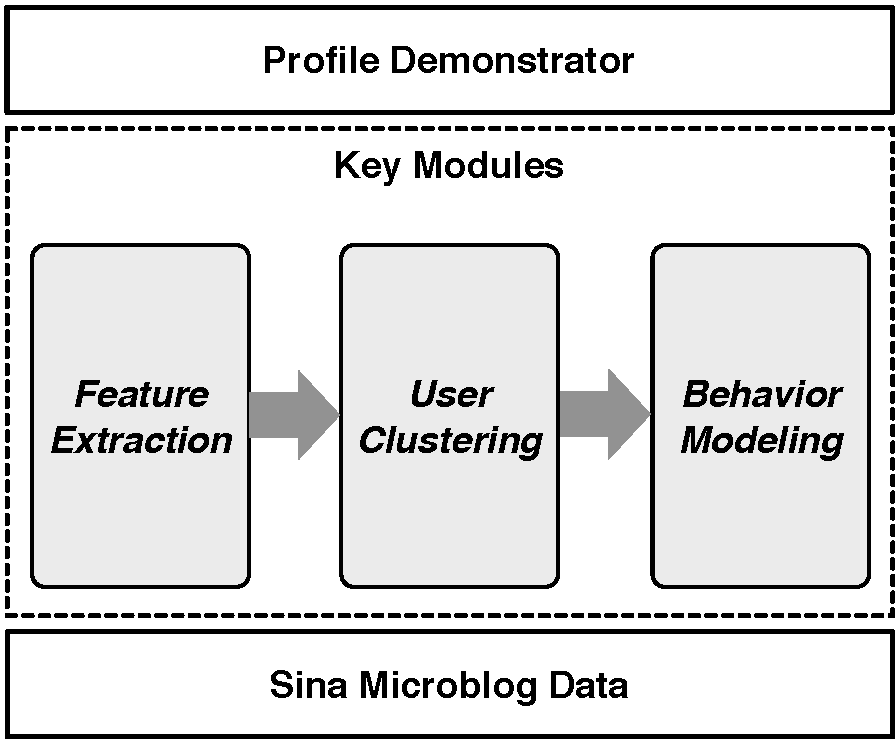
\includegraphics[width=.67\linewidth]{figures/architecture.pdf}
\vspace{-1ex}
\caption{\sys{} Architecture}
\label{fig:framework}
\vspace{-4ex}
\end{figure}


% #like and #comment are saved; could generalize \sys{} to model the liking behavior (among commented blogs)
\begin{comment}
\begin{figure}[!htb]
\centering
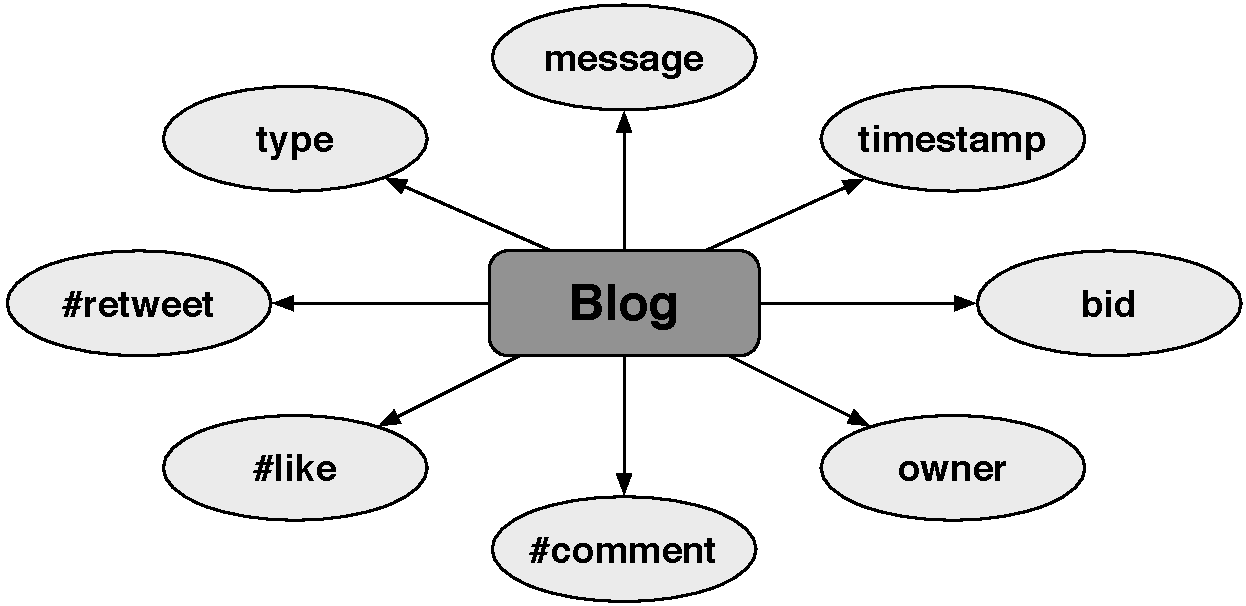
\includegraphics[width=.99\linewidth]{figures/microblog}
\caption{Blog Data in \sys{}}
\label{fig:blog}
\end{figure}
\end{comment}

\begin{comment}
\begin{figure}[!htb]
\centering
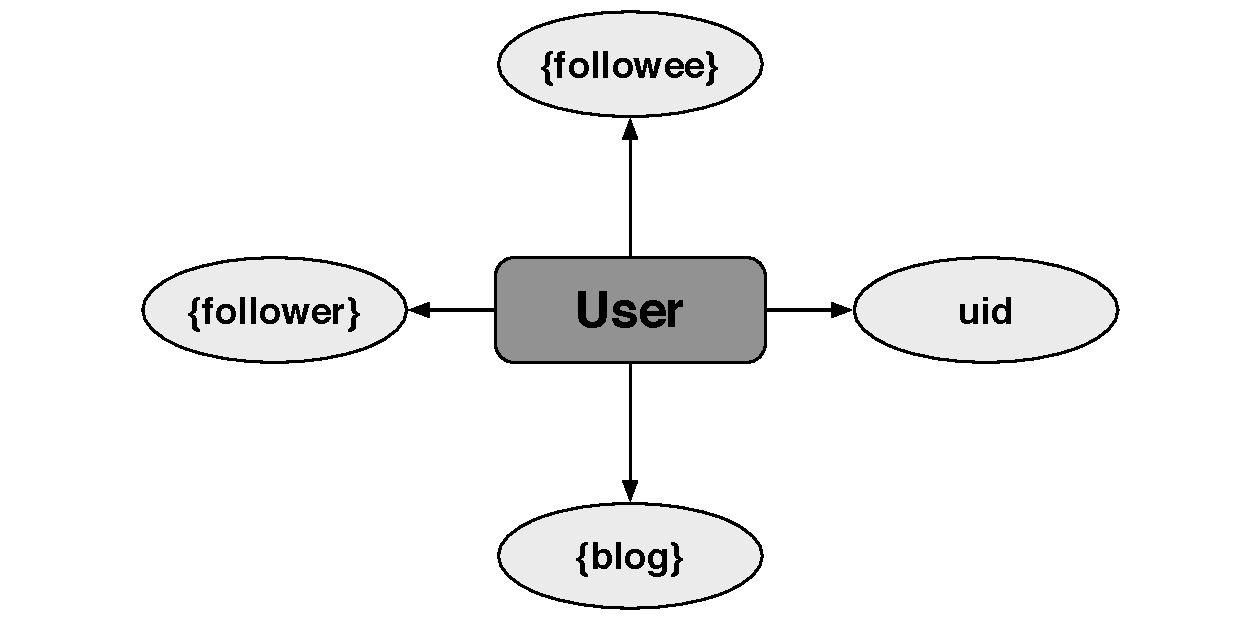
\includegraphics[width=.99\linewidth]{figures/user}
\caption{User Data in \sys{}}
\label{fig:user}
\end{figure}
\end{comment}


\stitle{Sina Microblog Data.} It is the data to be processed by \sys{}, i.e., data of microblogs and users, as shown in \textit{Definitions} \textit{\ref{def:blog}} and \textit{\ref{def:user}}.

\stitle{Key Modules.}
\sys{} consists of three key modules.
%\begin{enumerate}

	\stab(1)  Feature Extraction: By coalescing the microblog data, each user is depicted by a bunch of features, which are grouped into three categories. They are features of \textit{Basics} (e.g., the number of followers and followees), \textit{Behavior} (e.g., the frequency and the popular slots of \retg{}) and \textit{Interest} (e.g., the long-term/recent interests, as well as the explicit/implicit interests). These features are extracted from the stored  Sina Weibo data by Feature Extraction module, and serve as the input of the User Clustering module.
	
	\stab(2)  User Clustering: Providing the user-based features, User Clustering takes charge of the clustering task such that each user falls into a proper group.
	
	\stab(3)  Behavior Modeling: For each group obtained by User Clustering, Behavior Modeling builds a  model by employing both positive and negative samples (i.e., microblogs that are labeled with \retd{} and not \retd{}), over which the testing of users' \retg{} behavior is performed.
%\end{enumerate}
	
\stitle{Demonstrator.} At the top layer of \sys{}, it is the Demonstrator for visualizing all aspects of the system, e.g., profiling of user groups.
%For the time being, Profile Demonstrator presents \tbc{}.


As shown above, the distinctive feature of System  \sys{} is to model user \retg{} behaviors over groups instead of the mono model for all users.

\begin{table}[tb!]
\centering
\begin{small}
\caption{Illustration of Variables in Basic Feature}
\vspace{0.3cm}
\label{tbl:fe-info}
\begin{tabular}{ll}
\toprule
\multicolumn{1}{l}{\textbf{Variables}} & \multicolumn{1}{l}{\textbf{Illustration}}	\\	\midrule \midrule
\#$R_u$				& number of followers				\\	\midrule
\#$E_u$				& number of followees				\\	\midrule
                    & a ratio defined as the number of followers over \\
\raisebox{1.5ex}{$R_{ee}$}  & that of followees, i.e., ${\#R_u}/{\#E_u}$ \\  \midrule
$U_t$					& user type (as detailed in Table \ref{tbl:ucate})			\\ \bottomrule
\end{tabular}
\end{small}
\vspace{-3ex}
\end{table}
\begin{table}[tb!]
\centering
\begin{small}
\caption{Category of User Type}
\vspace{0.3cm}
\label{tbl:ucate}
\begin{tabular}{ll}
\toprule
\multicolumn{1}{l}{\textbf{Values}} & \multicolumn{1}{l}{\textbf{Illustration}}	\\	\midrule \midrule
0                       & $\#E_u \le 50 \ {\bf and} \ \#R_u \le 50$				\\	\midrule
\multirow{2}{*}{1}      & \multirow{2}{*}{$\frac{\#E_u}{\#R_u} \ \ge 5$}	\\
 						&                       									\\	\midrule
\multirow{2}{*}{2}		& \multirow{2}{*}{$\frac{\#R_u}{\#E_u} \ \ge 5$}  \\
						&															\\	\midrule
3                   	& other cases 												\\ \bottomrule
\end{tabular}
\end{small}
\end{table}



% jing @ 0927
% back to algorithm for interest features
% add motivation, intuition, etc

%clear points
%road map
%detail of each step, with motivation

\section{Feature Extraction}
\label{sec:fe}

With the underlying Sina Microblog Data, Feature Extraction is responsible for ``mining'' the user characteristics, resulting three features for each user.
These features are \textit{Basic Feature}, \textit{Behavior Feature} and \textit{Interest Feature}, which constitute the \textit{Feature Data} in \sys{}, i.e., \textit{Feature Data} = \{\textit{Basic Feature}, \textit{Behavior Feature}, \textit{Interest Feature}\}.

\subsection{Basic Feature}

\textit{Basic Feature} employs a vector $I$ to cover the basic info of user.
\begin{equation}
\label{eq:info}
	I = (\#R_u,\ \#E_u,\ R_{ee},\ \ U_t)
\end{equation}
where each variable is illustrated in Table \ref{tbl:fe-info}.
%Specifically, we use $\#(B_s | R(B)==1)$ and $\#(B_s | R(B)==0)$ to represent the number of \retd{} microblogs and microblogs that are originally created by the user.

\begin{table}[tb!]
\centering
\begin{small}
\caption{Illustration of Variables in Basic Feature}
\vspace{0.3cm}
\label{tbl:fe-info}
\begin{tabular}{ll}
\toprule
\multicolumn{1}{l}{\textbf{Variables}} & \multicolumn{1}{l}{\textbf{Illustration}}	\\	\midrule \midrule
\#$R_u$				& number of followers				\\	\midrule
\#$E_u$				& number of followees				\\	\midrule
                    & a ratio defined as the number of followers over \\  
\raisebox{1.5ex}{$R_{ee}$}  & that of followees, i.e., ${\#R_u}/{\#E_u}$ \\  \midrule
$U_t$					& user type (as detailed in Table \ref{tbl:ucate})			\\ \bottomrule
\end{tabular}
\end{small}
\end{table}


%mutex category
%type 0 is assumed to be representative

%replace 50 and 5 by variables of threshold

\begin{table}[tb!]
\centering
\begin{small}
\caption{Category of User Type}
\vspace{0.3cm}
\label{tbl:ucate}
\begin{tabular}{ll}
\toprule
\multicolumn{1}{l}{\textbf{Values}} & \multicolumn{1}{l}{\textbf{Illustration}}	\\	\midrule \midrule
0                       & $\#E_u \le 50 \ {\bf and} \ \#R_u \le 50$				\\	\midrule
\multirow{2}{*}{1}      & \multirow{2}{*}{$\frac{\#E_u}{\#R_u} \ \ge 5$}	\\
 						&                       									\\	\midrule
\multirow{2}{*}{2}		& \multirow{2}{*}{$\frac{\#R_u}{\#E_u} \ \ge 5$}  \\
						&															\\	\midrule
3                   	& other cases 												\\ \bottomrule
\end{tabular}
\end{small}
\end{table}


\subsection{Behavior Feature}

Unlike \textit{Basic Feature}, \textit{Behavior Feature} shows several statistics regarding the user's \retg{} behavior.
Such statistics include:
\begin{itemize}
	\item a value for the number of owned microblogs $\#B_u$
	\item a ratio $R_{oc}$ that is defined as the number of \retd{} microblogs over that of originally created, i.e., $\frac{\#(B_u | flag ==1)}{\#(B_u | flag ==0)}$
	\item a value showing the average number of \retd{} microblogs per week: $\#W_r$
	\item a normalized vector regarding the time distribution of a user's \retg{} behavior: $P_t\ = (p'_0,\ p'_1,\ ...,\ p'_{11})$, where $p'_0$ is the probability that the \retg{} activity happens from 0am to 2am, $p'_1$ is the probability that the \retg{} activity happens from 2am to 4am, and so on.
	\item a normalized vector with respect to the gap distribution of a user's \retg{} behavior: $P_g\ = (p''_0,\ p''_1,\ ...,\ p''_{5})$, in which $p''_0$ is the probability that the gap between two \retd{} microblogs is within 1 min. Ditto for $p''_1$ (1 min to 1 hour), $p''_2$ (1 to 12 hours), $p''_3$ (12 to 24 hours), $p''_4$ (24 to 48 hours) and  $p''_5$ (more than 48 hours).
\end{itemize}

Hence, \textit{Behavior Feature} $H$ per user comes with:
\begin{equation}
\label{eq:beha}
	H = (\#W_r,\ P_t,\ P_g)
\end{equation}
where $\#W_r$, $P_t$ and $P_g$ are illustrated as above.

\subsection{Interest Feature}

Different from the straightforward notions of \textit{Basic Feature} and \textit{Behavior Feature}, \textit{Interest Feature} involves a process of labeling users by their interested topics.
In short, with a given lexicon(made by some professionals) consisting of several \textit{topics}, the interest feature of a user is a normalized vector, in which each dimension refers to the probability that the said user matches a \textit{topic}.

\begin{definition}
\label{def:lexi}
A lexicon $L$ consists of a set of topics $t$ such that each topic is associated with a set of cell words $c$. Each cell word depicts an aspect of the topic.
\end{definition}

\begin{definition}
\label{def:bw}
%used \label{def:blog} previously
With a given user $u$, each microblog $b \in B_u$ could be decomposed into a set of words $w$.
\end{definition}

\begin{definition}
\label{def:inte}
The interest feature of a given user is a normalized vector
\begin{equation}
\label{eq:inte}
P_f\ = (p_0,\ p_1,\ ...,\ p_{x-1})
\end{equation}
in which the said user matches $x$ \textit{topics} in lexicon and $p_i$ refers to the similarity of the user and each matched topic (interest). The definition of such similarity shall be detailed in each scenario (explicit/implicit interest analysis, towards words/topics, etc).
\end{definition}


Next, we shall present the ``mining'' process for interest features.
In short, \sys{} employs a well established lexicon to discover the explicit interests of users.
In case no proper explicit interests are found, TF-IDF and Twitter-LDA are leveraged to explore the implicit interests, during which word2vector participates to provide the similarity between two words.

In \sys{}, a word, either in the form of $c$ or $w$, acts as the minimum unit for analysis.
Hence, the similarity of a word pair ($w$, $c$), i.e., $sim(w, c)$, could be generalized to the similarity of a microblog against one topic $sim(b, t)$, and finally to a user versus each topic in lexicon $sim(u, t)$; topics with similarity satisfying certain thresholds are allocated to the user $u$ and constitute the interests of $u$.

For instance, the following steps depict the ``mining'' process of the interest feature $P_f$ for a user $u$.

\stitle{Step 1:} Each microblog of $u$ is decomposed into a word set. %, i.e., $b = \{w\}$ where $b \in B_s(u)$.

\stitle{Step 2:} Explicit interests are explored. Specifically, every word $w$ is sent to match each cell word $c$ of lexicon topics.
If $w$ and $c$ are identical, $sim(w, c) = 1$.
Otherwise, $sim(w, c) = 0$.
As to the similarity of $b$ against a lexicon topic $t$, it is:
\begin{equation}
\label{eq:bt}
sim(b, t) = \sum_{\substack{i, j}} sim(w_i, c_j)
\end{equation}
where $sim(w_i, c_j)$ refers to the similarity of a word pair.

If $sim(b, t)$ satisfies a certain threshold (3 by default) , topic $t$ is labeled to microblog $b$;
the user $u$ is then discovered having an explicit interest (topic) $t$.
Thus, by looking into the similarity of $b$ against all topics in lexicon, the explicit interests of $u$ is returned, in the form of interest feature (see Definition \ref{def:inte}).

If none of $sim(b, t)$ could meet the threshold, i.e., explicit interest discovery over user $u$ fails, go to \textbf{Step 3} and \textbf{Step 4} in parallel, so as to ``mine'' the implicit interests of $u$.

\stitle{Step 3:} A metric \textit{TF-IDF weight} $W_f$ is computed, i.e., employing TF-IDF (term-frequency and inverse document-frequency) to calculate the weight distribution of words in microblog $b$:
\begin{equation}
\label{eq:tf}
W_f = \{(w_i, p_i)\}
\end{equation}
where $w_i$ refers to a single word, of which the weight is $p_i$, with $\sum_{\substack{i}} p_i = 1$.

To compute such weight $p_i$ for word $w_i$, a metric $p''_i$ is first calculated as:
\begin{equation}
\label{eq:tf-w}
p''_i = \frac{|b_i|}{|b|} * log(\frac{|D_i|}{|D|})
\end{equation}
in which we use the operator $|\ |$ to measure the cardinality, such that $|b_i|$ is the occurrences of word $w_i$ in microblog $b$ and $|b|$ the total occurrences of all words in $b$.
Ditto for $|D_i|$ and $|D|$, except that the scope is the overall dataset, rather than a single microblog $b$.

Hence, each word $w_i$ shall get an initial weight of $p''_i$, upon which the normalization is performed and $p_i$ is obtained, resulting the \textit{TF-IDF weight} (see Definition \ref{eq:tf}).
Go to \textbf{Step 5}.

\stitle{Step 4:} Similarly, another metric \textit{Twitter-LDA weight} $W_w$ is obtained, i.e., using Twitter-LDA  %\ref{IEEEexample:zhao2011comparing}
\cite{IEEEexample:zhao2011comparing}
to result the word weight distribution of microblog $b$.
Unlike TF-IDF, Twitter-LDA first trains the overall microblogs, allocating each microblog with a \textit{tag}.
%
The structure of \textit{tag} is as follows:
\begin{equation}
\label{eq:tw-tag}
W_t = \{(w'_i, p'_i)\}
\end{equation}
where $w'_i$ refers to a word in \textit{tag} $W_t$, and $p'_i$ is the probability that $w'_i$ appears in microblogs with the said \textit{tag}, with $\sum_{\substack{i}} p'_i = 1$ ($|W_t|\ =\ 30$ in this work by default).
%
Subsequently, $W_t$ are leveraged to conclude $W_w$, i.e., $W_w\ =\ W_t$ , which shares the format with that of $W_f$.
Go to \textbf{Step 6}.

\stitle{Step 5:} TF-IDF based similarity is calculated.
For example, the similarity (in the form of a value) of $W_f$ over a single topic $t$ in lexicon, written as $sim(W_f, t)$, is defined as:
\begin{equation}
\label{eq:sim-tf1}
sim(W_f, t) = \sum_{\substack{i}} p_i*sim(w_i, t)
\end{equation}
where $W_f = \{(w_i, p_i)\}$, $t = \{c_j\}$, and $sim(w_i, t)$ is the averaged word similarity $sim(w_i, c_j)$ returned by word2vector \cite{IEEEexample:mikolov2013distributed}.
Go to \textbf{Step 7}.

\begin{comment}
:
\begin{equation}
\label{eq:sim-tf2}
sim(w_i, t) = \sum_{\substack{j}} sim(w_i, c_j)
\end{equation}
\end{comment}



\stitle{Step 6:} Accordingly, Twitter-LDA based similarity is available.
Again, a single topic $t$ in lexicon is used for yardstick and the similarity of $W_w$ over $t$, written as $sim(W_w, t)$, is defined as:
\begin{equation}
\label{eq:sim-tw1}
sim(W_w, t) = \sum_{\substack{i}} p'_i*sim(w'_i, t)
\end{equation}
%where $W_w = \{(w'_i, p'_i)\}$, $t = \{c_j\}$,
where $W_w$ is a set of $(w'_i, p'_i)$, $t$ covers each $c_j$,
and $sim(w'_i, t)$ is the averaged word similarity $sim(w'_i, c_j)$ returned by word2vector.
Go to \textbf{Step 7}.

\begin{comment}
:
\begin{equation}
\label{eq:sim-tw2}
sim(w'_i, t) = \sum_{\substack{j}} sim(w'_i, c_j)
\end{equation}
\end{comment}



\stitle{Step 7:} Hence, the similarity of a microblog $b$ against a lexicon topic $t$ is given by:
\begin{equation}
\label{eq:simbt}
sim(b, t) = \alpha * sim(W_f, t) + (1 - \alpha) * sim(W_t, t)
\end{equation}
where the $\alpha$ is a parameter by which \sys{} could set flexible priorities between TF-IDF and Twitter-LDA.
Go to \textbf{Step 8}.

\stitle{Step 8:} Repeat the above steps (Step 1 to Step 7) for the microblog $b$ over every topic in lexicon, i.e., $\forall t_k \in L$ results one similarity value of $sim(b, t_k)$.
Such computation further extends to all the microblogs owned by user $u$, such that:
$\forall b_m \in B_s(u)$, $\forall t_k \in L$, there exists a similarity of $sim(b_m, t_k)$.
Hence, the overall similarity of user $u$ over lexicon topics $\{t\}$ (i.e., $L$), written as $S(u,\ L)$, could be denoted by a vector:
\begin{equation}
\label{eq:simul}
S(u, L) = (s_0,\ s_1,\ ...,\ s_{n-1})
\end{equation}
where $n$ refers to the cardinality of $L$ (i.e., number of topics in $L$) and $s_k$ is the overall similarity of user $u$ over topic $t_k$, which is given by:
\begin{equation}
\label{eq:simul-2}
s_k = \sum_{\substack{m}} sim(b_m, t_k)
\end{equation}

Among the $n$ dimensions of $S(u,\ L)$, those with top $x$ (3 in \sys{}) similarity values are selected to label the implicit interests of user $u$, which results an $x$ dimensional vector $P_f$ as described in Definition \ref{def:inte}.
Similarly, interest features of all users are returned.

As a result, the \textit{Feature Data} for every user $u$, written as $F(u)$, is given by:
\begin{equation}
\label{eq:fu}
	F(u) = (I,\ H,\ P_f)
\end{equation}
where $I$, $H$ and $P_f$ refer to \textit{Basic Feature}, \textit{Behavior Feature} and \textit{Interest Feature} separately (see formulas \ref{eq:info}, \ref{eq:beha} and \ref{def:inte}).
And it could be written as a vector:
\begin{equation}
\label{eq:fu-flat}
	F(u) = (\#R_s, \#E_s, R_{ee}, \#B_s, R_{oc}, U_t, \#W_r, P_t, P_g, P_f)
\end{equation}
where each dimension refers to a data item of \sys{}.


\section{User Clustering}
\label{sec:uc}

%clear points
%road map
%detail of each step, with motivation
%proof if applicable
%self-explain

Providing the \textit{Feature Data}, User Clustering takes the charge of grouping each user concerned into a proper cluster.
Algorithm \ref{alg:uc} illustrates such overall procedure.
%
The idea is to enumerate a number of clustering trials (line \ref{enu}) and select the optimal solution with the best Silhouette coefficient value ($v$ in line \ref{opti}).
In principle, each trial (referred by $t$ in line \ref{enu}) first performs a clustering task (line \ref{task}; to be detailed in section \ref{sec:cluster}), resulting a cluster (by $l(u)$) for each user $u$ (line \ref{l});
then, each user obtains a Silhouette coefficient value $v(u)$ stemmed from the in/out-cluster distances (lines \ref{v-b}--\ref{v-e}; shall be illustrated in section \ref{sec:compu});
finally, the averaged Silhouette coefficient value of all users serves as the Silhouette coefficient value of the current trial, written as $v(t)$ (line \ref{avg}), by which the said selection process is conducted (line \ref{opti}).


\begin{algorithm}[t]
\begin{small}
\caption{User Clustering in \sys{}}
\label{alg:uc}

\begin{algorithmic}[1]
\State Input: \textit{Feature Data} of users $\{F(u)\}$, the minimum/maximum number of clusters $N_i$ and $N_a$
\State Output: Optimal user clustering result $R$
\\
\ForAll {$t \in [N_i, N_a]$} \label{enu}
	\State group users $\{u\}$ into $t$ clusters by $\{F(u)\}$ \label{task}
	\State clustering result $R'(t)\ =\ \{(u,\ l(u))\}$ with cluster info $l(u)$ for each user $u$ \label{l}
	\ForAll {$u \in \{u\}$}
		\State in-cluster distance $d_i(u)$ \label{v-b}
		\State out-cluster distance $d_o(u)$
		\State Silhouette coefficient value $v(u)\ =\ \frac{(d_o - d_i)}{max(d_o,\ d_i)}$ \label{v-e}
	\EndFor
	\State $v(t)\ =\ Avg\{v(u)\}$ \label{avg}
\EndFor
\If {$v(a)\ ==\ \ Max\{v(t)\}$} \label{opti}
	\State $R$ = $R'(a)$
\EndIf
\State \bfseries{return} $R$
\end{algorithmic}
\end{small}
\end{algorithm}

Next, we shall now first detail how \sys{} performs the clustering task and subsequently illustrate the computation for the metric of Silhouette coefficient value.

\subsection{Clustering in \sys{}}
\label{sec:cluster}

In \sys{}, the clustering rests on an optimized K-Prototype \cite{IEEEexample:huang1997clustering} algorithm, named K-Gru in this work.
Similar as K-Prototype, K-Gru randomly selects the cluster kernels among samples and employs the minimum distance between them to determine an initial result, upon which the clustering tasks are iterated until the results are stable.

Unlike K-Prototype that supports vector samples in which each dimension is of numerical/categorical, K-Gru could also handle the case where a dimension is one normalized vector.
%
Recall the sample data for User Clustering, i.e., \textit{Feature Data} in form of vectors (see formula \ref{eq:fu-flat}), of which the data type regarding each dimension is shown as Table \ref{tbl:data-type}.

\begin{table}[!htb]
\centering
\begin{small}
%\caption{Types of Dimensional Data in \textit{Feature Data} Vector}
\caption{Dimension Types in \textit{Feature Data} Vector}
\vspace{0.3cm}
\label{tbl:data-type}
\begin{tabular}{ll}
\toprule
\multicolumn{1}{c}{\textbf{type}} & \multicolumn{1}{c}{\textbf{data dimensions}}	\\	\midrule \midrule
numerical data				& $\#R_u$, $\#E_u$, $R_{ee,u}$, $\#B_u$,\\
                            &  $R_{oc,u}$, $\#W_{r,u}$,$\#W_{t,u}$				\\	\midrule
categorical data			& $G_u$,$P_u$,$U_{t,u}$				\\	\midrule
normalized vectors			& $P_{rt,u}$, $P_{rg,u}$,$P_{tt,u}$,$P_{tg,u}$,$P_{f,u}$			\\ \bottomrule
\end{tabular}
\end{small}
\end{table}

As aforementioned, the clustering of K-Gru rests on the distance between vector samples, where the dimensions are combined with numbers(normalized to 0-1 range), categories and normalized vectors.
For simplicity, we shall first illustrate the distance calculation of the simple vectors with mono data type on each dimension and then demonstrate that of complex vectors in K-Gru.

Given two numerical vectors $Y'\ = (y'_0, y'_1, ...)$ and $Z'\ = (z'_0, z'_1, ...)$, the \od{} \cite{IEEEexample:books/mk/HanKP2011} between $Y'$ and $Z'$ is given by :
%
\begin{equation}
\label{eq:od}
D_n(Y', Z') = \sum_{\substack{e}} (y_e - z_e)^2
\end{equation}

As to the categorical vectors $Y''\ = (y''_0, y''_1, ...)$ and  $Z''\ = (z''_0, z''_1, ...)$, the \hd{} \cite{IEEEexample:huang1997clustering} of $Y''$ and $Z''$ is:
%
\begin{equation}
\label{eq:hd}
D_h(Y'', Z'') = \sum_{\substack{e}} H_e
\end{equation}
where $H_e$ refers to the \hd{} over each dimension, with $H_e\ =\ 1$ if $y''_e$ and $z''_e$ share the identical value, and $H_e\ =\ 0$ otherwise.

Regarding two vectors where each dimension is a normalized vector per se, Cosine Similarity is leveraged to compute the distance.
Then, the distance between such two vectors $Y^{\ast}\ = (Y^{\ast}_0, Y^{\ast}_1, ...)$ and $Z^{\ast}\ = (Z^{\ast}_0, Z^{\ast}_1, ...)$ is:
%
\begin{equation}
\label{eq:vd}
D_v(Y^{\ast}, Z^{\ast}) = 1- \sum_{\substack{e}} Y^{\ast}_e \cdot Z^{\ast}_e
\end{equation}
where $\cdot$ refers to the dot product operation between two normalized vectors $Y^{\ast}_e$ and $Z^{\ast}_e$.

Hence, the said distance regarding the complex vectors ($Y\ =\ (Y_0, Y_1, ...)$ and $Z\ =\ (Z_0, Z_1, ...)$ ) in K-Gru, named \gd{}, could be deduced as:
%
\begin{equation}
\label{eq:gd}
D_g(Y, Z) = \sum_{\substack{e}} G_e
\end{equation}
where the distance on each dimension $G_e$ is given by:
%
\begin{equation}
\label{eq:ge}
G_e =
  \begin{cases}
    (Y_e - Z_e)^2       & \quad \text{if } Y_e/Z_e \text{ is numerical}\\
    H_e\ (1\ or\ 0)       	& \quad \text{if } Y_e/Z_e \text{ is categorical}\\
    1 - Y_e \cdot Z_e  		& \quad \text{if } Y_e/Z_e \text{ is of normalized vector}
  \end{cases}
\end{equation}


\subsection{Silhouette Coefficient Metric Computation}
\label{sec:compu}

In \sys{}, Silhouette coefficient value serves as the fundamental criteria for the optimal clustering selection.
Providing a clustering result, each user is associated with a cluster.

For a given user $u$ of cluster $l$, we employ the vector $Y$ to denote the \textit{Feature Data} as in formula \ref{eq:fu-flat}.

\begin{definition}
\label{def:di}
The in-cluster distance $d_i(u)$ is the average distance to all the other users in the same cluster, i.e., $\forall u'' \in l$ \& $u \neq u''$:
\begin{equation}
	d_i(u) = Avg\{D_g(Y_u, Y_u'')\}
\end{equation}
\end{definition}

\begin{definition}
\label{def:do}
The out-cluster distance $d_o(u)$ is measured as the minimum of the distances $\{d^{\ast}\}$ between $u$ and other clusters ($\forall l' \neq l$), i.e.:
\begin{equation}
	d_o(u) = Min\{d^{\ast}(u, l')\}
\end{equation}
where $d^{\ast}$ is given by:
\begin{equation}
	d^{\ast}(u, l') = Avg\{D_g(Y_u, Y_u')\}\ \forall u' \in l'
\end{equation}
\end{definition}

\begin{definition}
\label{def:coef}
The Silhouette coefficient value $v(u)$ is thus concluded:
\begin{equation}
\label{eq:coef}
v(u)\ =\ \frac{(d_o - d_i)}{max(d_o,\ d_i)}	
\end{equation}
\end{definition}

Intuitively, a good clustering solution should result bigger $d_o$ and smaller $d_i$, such that samples with obvious differences go to various clusters and vice versa.
When $d_o$ is far more than $d_i$, Silhouette coefficient value approaches to 1.
Hence, the larger Silhouette coefficient value is, the better clustering performs, by which the optimal solution is selected.






\section{Group based Behavior Modeling}
\label{sec:gm}

%clear points
%road map
%detail of each step, with motivation


Recall the central problem of \sys{}, where the \retg{} behaviors of users are modeled.
Specifically, such model is built by Group Modeling for each user group and thus named as group model.
To avoid ambiguity, we shall use the term of \textit{items} to denote the data for training the group model.
A given \textit{item} is either positive or negative.

\begin{definition}
\label{def:gm-it}
An item $E$ involves a microblog $b$ and a user $f$ such that $f\ \in R_{b.O}$, i.e., $f$ is a follower of  the owner of microblog $b$.
\begin{equation}
\label{eq:gm-it}
E \in
  \begin{cases}
    \text{positive items}       & \quad \text{if } f \text{ \retd{} } b\\
    \text{negative items}  		& \quad \text{if } f \text{ did not \ret{} } b
  \end{cases}
\end{equation}
\end{definition}

And the data of item $E$ could be further divided into three parts.
%\begin{itemize}

	\stab(1) \stitle{User Info} contains a list of aforementioned metrics \{$G_u$, $P_u$,\#$R_u$, \#$E_u$, $R_{ee,u}$ \}.
	
	\stab(2) \stitle{Microblog Info} refers to metrics related to the microblog $b$. The number of times the $b$ be retweeted, be commented, be liked and the length of the microblog contents are considered. What's more, we also considers the correlation between microblog contents and recent events, where the latter is returned by Ring \cite{IEEEexample:ring}. The correlation metric $C_h$ is in the form of a normalized vector with each dimension represents one event (similar as $P_{f,u}$ in formula \ref{eq:inte}). Each event could be viewed as a topic $t$, over which the correlation of a microblog $b$ could be obtained by formula \ref{eq:sim-tw1}.

	\stab(3) \stitle{Interaction Info} includes seven correlation metrics. They are of \#$B_u$, $R_{oc,u}$, \#$W_{r,u}$, \#$W_{t,u}$, microblog $b$ versus the user $u$'s \textit{Interest Feature} $P_f(u)$ (a.k.a. long-term/stable interest in this work), $b$ versus $u$'s short-term interest $P_s(u)$ that is mined from $u$'s recent microblogs (e.g., within 30 days) in the same manner of $P_f(u)$, and $b$'s timestamp versus the time distribution of $u$'s \retg{} behavior $P_{rt,u}$.
%\end{itemize}

In this paper, we see modeling retweeting behavior of group as a classification problem and use random forest classifier to solve the problem. The advantage of using classification model is that we can integrate different combinations of the features into the model conveniently. As a result, the obtained group behavior model could learn what does a positive/negative item look like over each metric mentioned above.\par












\section{Performance Evaluation}
\label{sec:perf}

\par In this section, we shall first detail the experimental setting, and we then present the evaluation result and analysis, showing the benefit of \sys{} against state of the art approaches.

\subsection{Experimental Setting}

Experiments were run on a machine with two Intel Xeon E5C2630 2.4GHz CPUs and 64 GB of Memory, running 64 bit Windows 7 professional system.
%
We have employed a real-world dataset Sina Weibo that consists of 24 million microblogs that are associated with 43.5K users.

With respect to the parameters of \sys{}, we use the default values as mentioned in previous sections.
Particularly, for the Feature Extraction module, for practical reasons, we employed a smaller testing dataset (with manually labeled topics for yardstick) to obtain the proper value of $\alpha$ for extracting \textit{Interest Feature};
For the User Cluster module, we studied the clustering solutions with the minimum/maximum number of clusters 2 and 10;
For the Behavior Modeling module, the recent 30 days microblogs of users are used for their short-term interest analysis,
and popular words in the latest 24 hours are returned by Ring as the Hot Event keywords \cite{IEEEexample:ring}.

\subsection{Result and Analysis}
Next, we shall report the performance of system \sys{} over each component.



\stitle{Exp-1: Feature Extraction}
%
Fig.\ \ref{fig:fe} shows the testing results of using various $\alpha$ values.
We report the interest accuracy with various $\alpha$ values. Suppose the label set manually labeled for each microblog is $A$, the label set our method labeled is $B$.
The interest accuracy is defined as $\frac{ A \cap B }{ A \cup B }$.


System \sys{} reaches the optimal results when $\alpha$ is 0.7,
upon which the interest feature extracting is performed for the overall dataset with 43.5K users and 24 million microblogs.
In general, it performs well when $\alpha$ falls into $[0, 0.8]$.


\begin{figure}[H]
\begin{minipage}[t]{0.45\linewidth}
\centering
 \hspace{1.5in}
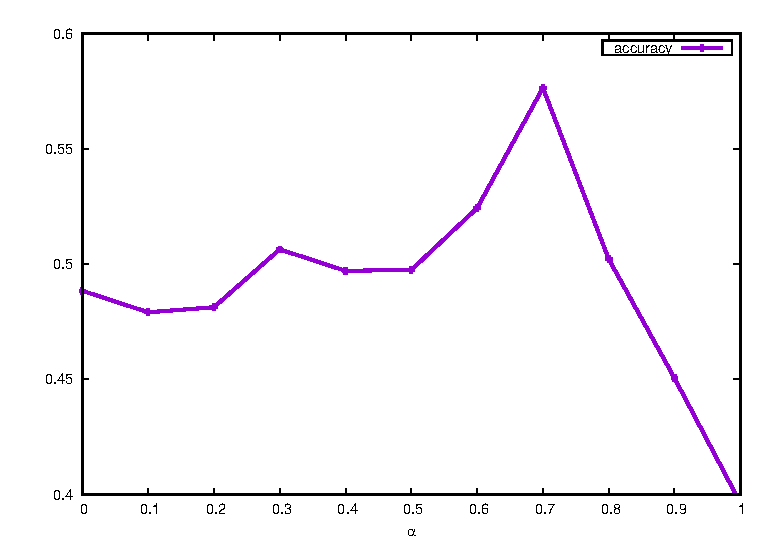
\includegraphics[width=1\textwidth]{figures/Interests}
\caption{Interest Extraction: Varying $\alpha$.}\label{fig:fe}
\end{minipage}
\hfill
\begin{minipage}[t]{0.45\linewidth}
\centering
 \hspace{1.5in}
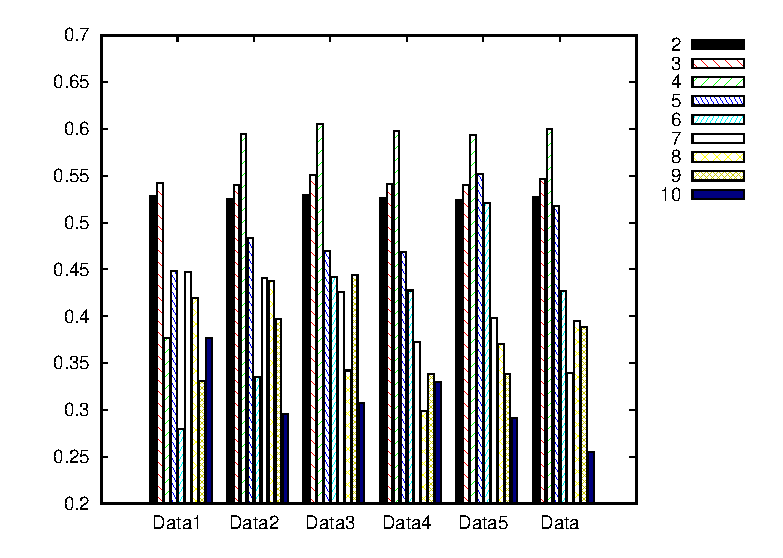
\includegraphics[width=1\textwidth]{figures/clustering}
\caption{Silhouette Coefficient Tests.}\label{fig:10-c}
\end{minipage}
\end{figure}

\stitle{Exp-2: User Clustering}
%
Fig.\ \ref{fig:10-c} depicts the Silhouette Coefficient Values of multiple clustering solutions, with the cluster number varied from 2 to 10.
Specially, we used different testing datasets, with \textit{Data} containing the overall 43.5K users, and each of \textit{\{Data1,\ldots, Data5\}} contains 10K randomly selected users.
Except for \textit{Data1}, solutions for \textit{\{Data2,\ldots, Data5\}} are the best for 4 clusters.



%\begin{figure}[tb!]
%\centering
%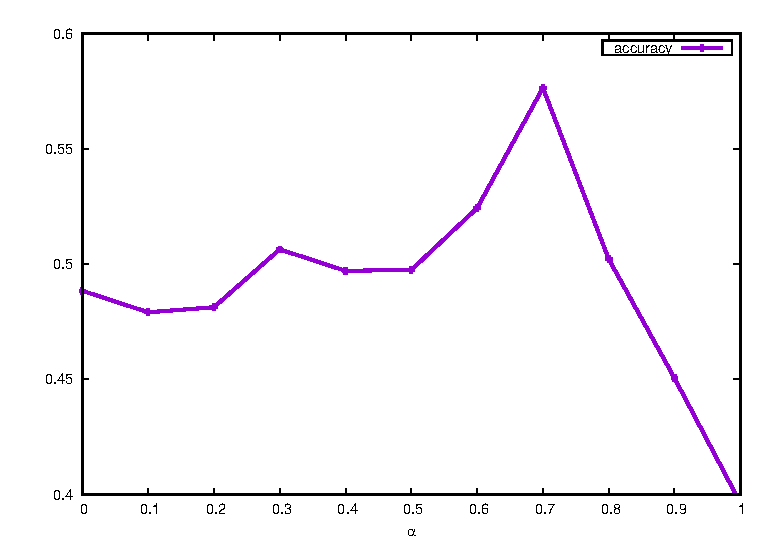
\includegraphics[width=.315\linewidth]{figures/Interests}
%\caption{Testing Results with Various $\alpha$.}
%\label{fig:fe}
%\vspace{-4ex}
%\end{figure}

%\begin{figure}[tb!]
%\centering
%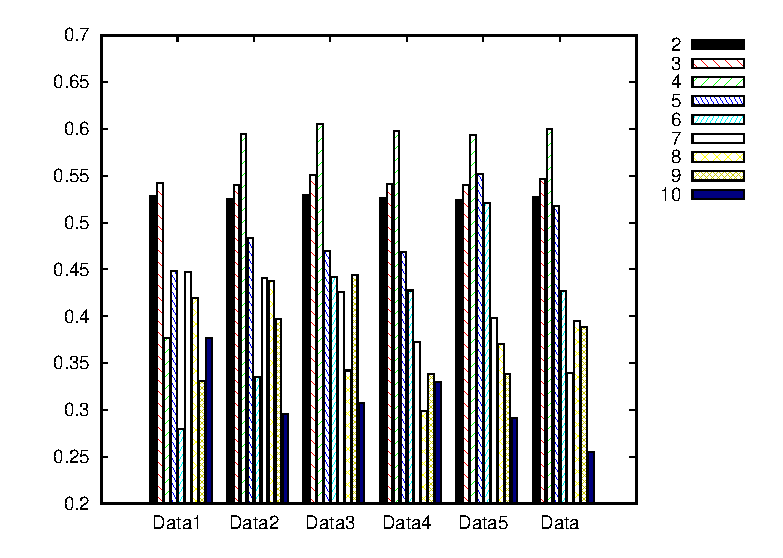
\includegraphics[width=.315\linewidth]{figures/clustering}
%\caption{Silhouette Coefficient Tests.}
%\label{fig:uc}
%\vspace{-5ex}
%\end{figure}



\begin{comment}
\begin{figure*}[tb!]
  \centering
  \subfigure[Precision]{
    \label{fig:10-a}
    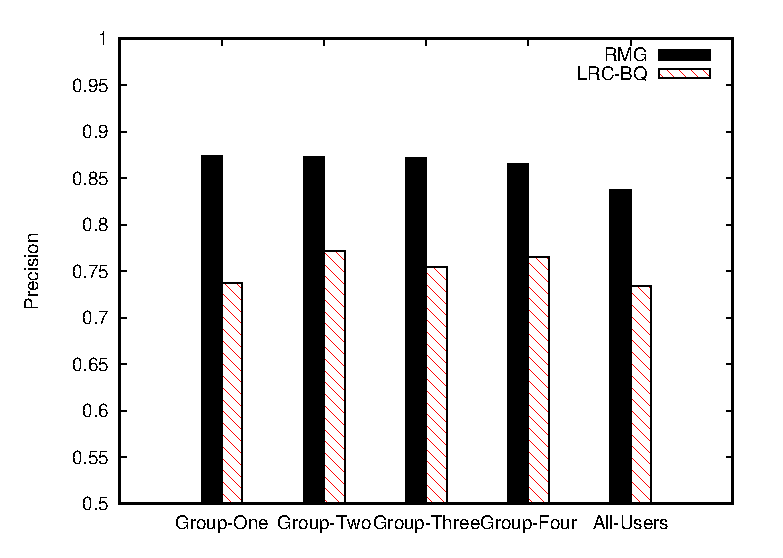
\includegraphics[width=0.315\textwidth]{figures/precision.eps}}
  %\hspace{1in}
  \subfigure[Recall]{
    \label{fig:10-b}
    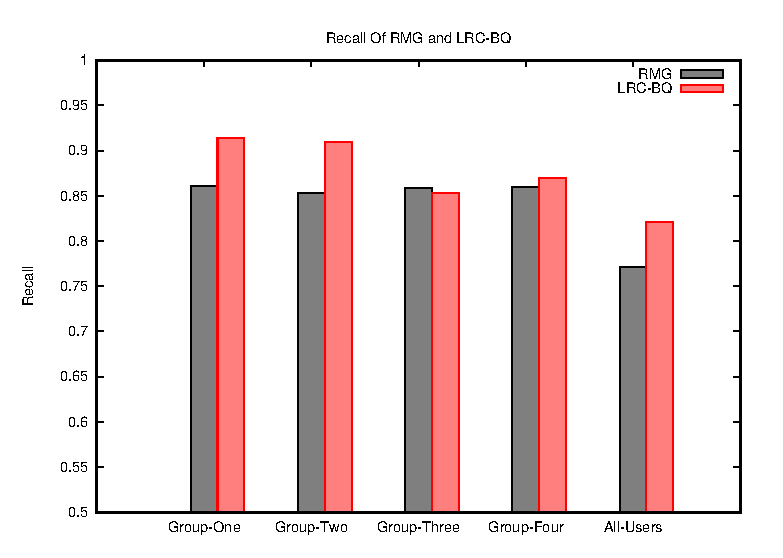
\includegraphics[width=0.315\textwidth]{figures/recall.eps}}
  %\hspace{1in}
  \subfigure[$F_1$ Score]{
    \label{fig:10-c}
    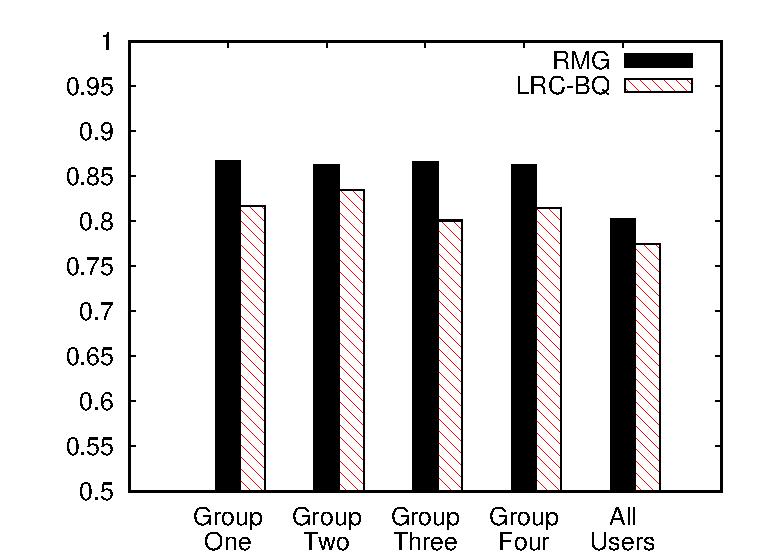
\includegraphics[width=0.315\textwidth]{figures/F-Measure.eps}}
  \caption{Performance of \sys{} Versus LRC-BQ.}
  \label{fig:10}
\vspace{-4ex}
\end{figure*}
\end{comment}



\stitle{Exp-3: Behavior Modeling}
%
Fig.\ \ref{fig:10-a} shows the performance of \sys{} against the state of the art approach LRC-BQ \cite{IEEEexample:conf/ijcai/ZhangLTCL13}.
We evaluate the performance using the metrics of accuracy.
LRC-BQ does not deal with user grouping.
Hence, we not only study the modeling effect per group (i.e., ``Group-One/Two/Three/Four'' with user clustering),
but also examine \sys{} versus LRC-BQ in the case that all users are in a single group (i.e., ``All-Users'').
The results show that:
%\begin{itemize}

	\stab(1) With user clustering, \sys{} performs better than LRC-BQ in most cases.
	
	\stab(2) For \sys{}, having user clustering is better than the alternative single group. Ditto for LRC-BQ.
%\end{itemize}

\begin{figure*}[tb!]
  \centering
  \subfigure[Accuracy of \sys{} Versus LRC-BQ.]{
    \label{fig:10-a}
    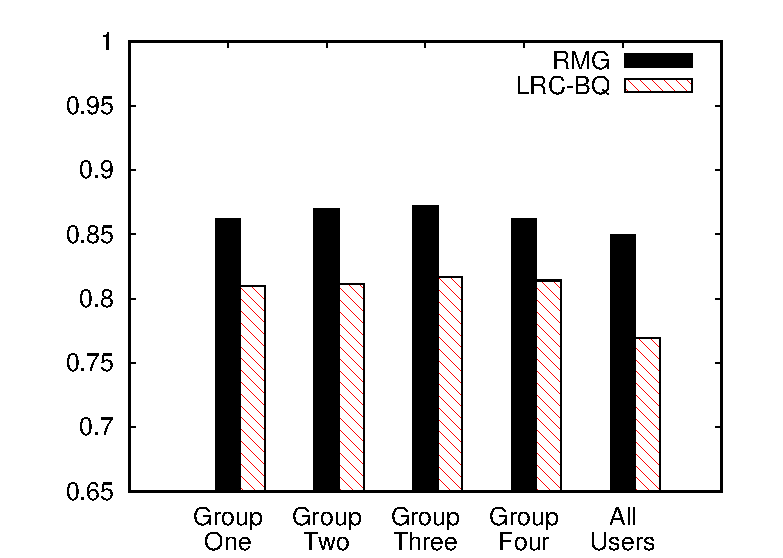
\includegraphics[width=0.355\textwidth]{figures/precision-1.eps}}
  \hspace{0.5in}
   \subfigure[Accuracy of Using Various Data Items for Modeling of \sys{}.]{
    \label{fig:11-a}
  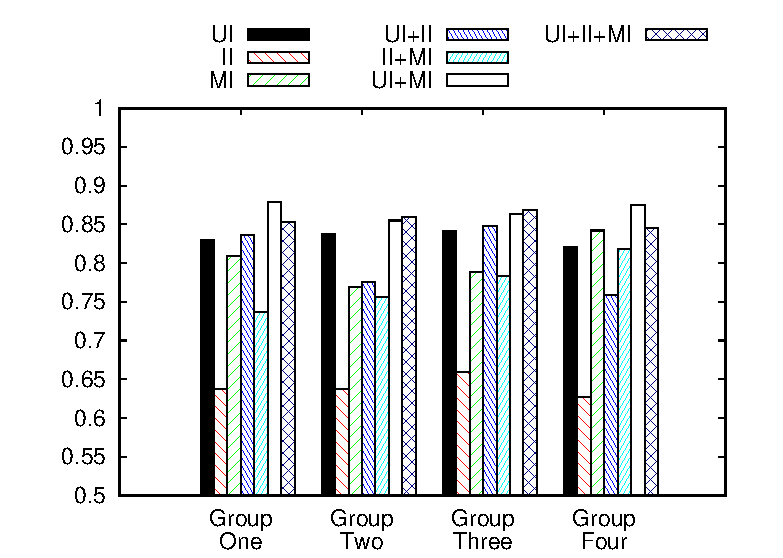
\includegraphics[width=0.45\textwidth]{figures/precisionofdifferentfeatures.eps}}
  \caption{Performance of \sys{} }
  \label{fig:fig-2}
\end{figure*}

Fig.\ \ref{fig:11-a} explores the performance of \sys{} when using alternative data items for modeling.
By default, \sys{} uses ``UI+II+MI'', i.e., items of users (UI), microblogs (MI) and interactions (II).
How about using other combinations of the above item(s)?
As shown in Fig.\ \ref{fig:11-a}, the default setting wins in most cases.

\begin{comment}
\begin{figure*}
  \centering
  \subfigure[Precision]{
    \label{fig:11-a}
    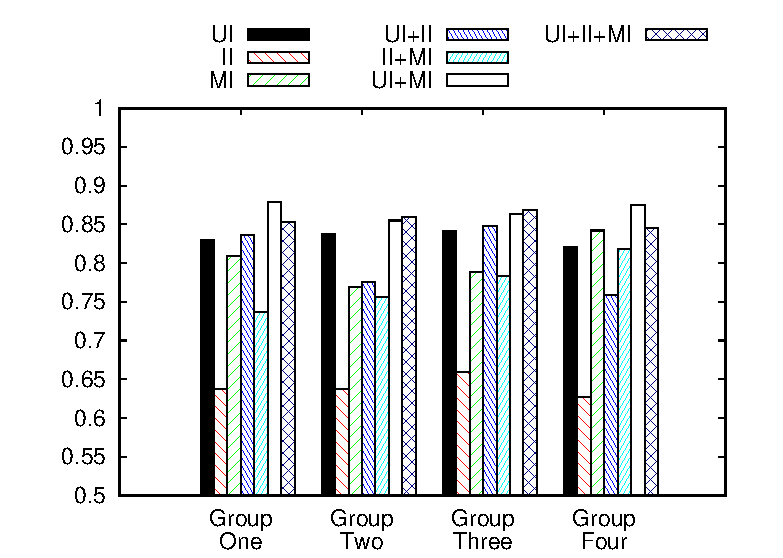
\includegraphics[width=0.315\textwidth]{figures/precisionofdifferentfeatures.eps}}
  %\hspace{1in}
  \subfigure[Recall]{
    \label{fig:11-b}
    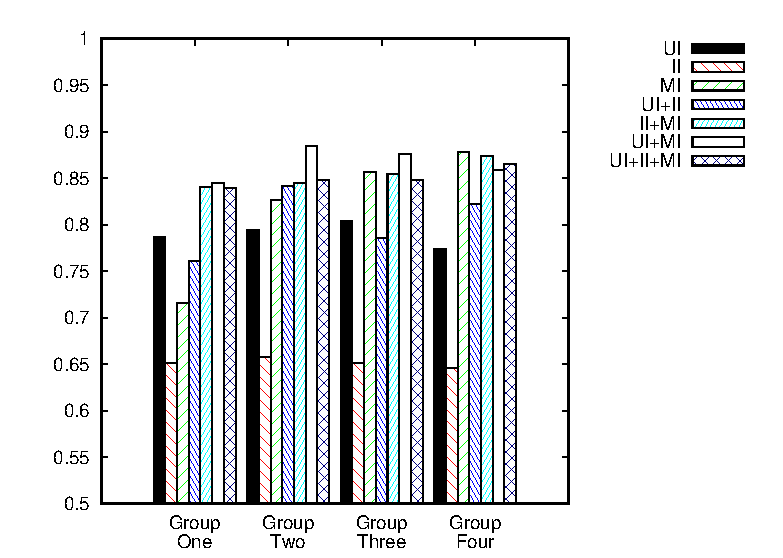
\includegraphics[width=0.315\textwidth]{figures/recallofdifferentfeatures.eps}}
  %\hspace{1in}
  \subfigure[$F_1$ Score]{
    \label{fig:11-c}
    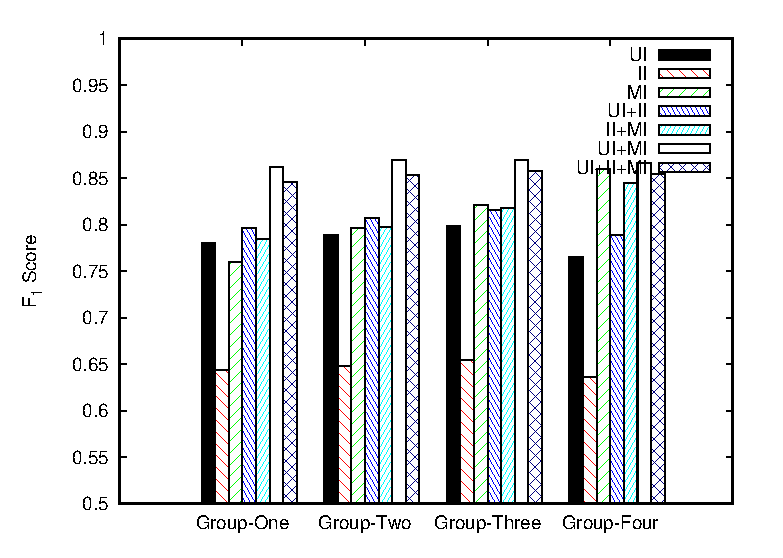
\includegraphics[width=0.315\textwidth]{figures/fmeasureofdifferentfeatures.eps}}
  \caption{\sys{} Performance of Using Various Data Items for Modeling.}
  \label{fig:11}
  \vspace{-4ex}
\end{figure*}
\end{comment}


\begin{figure*}
  \centering
  \subfigure[]{
      \label{fig:userFeatures:uf-1}
      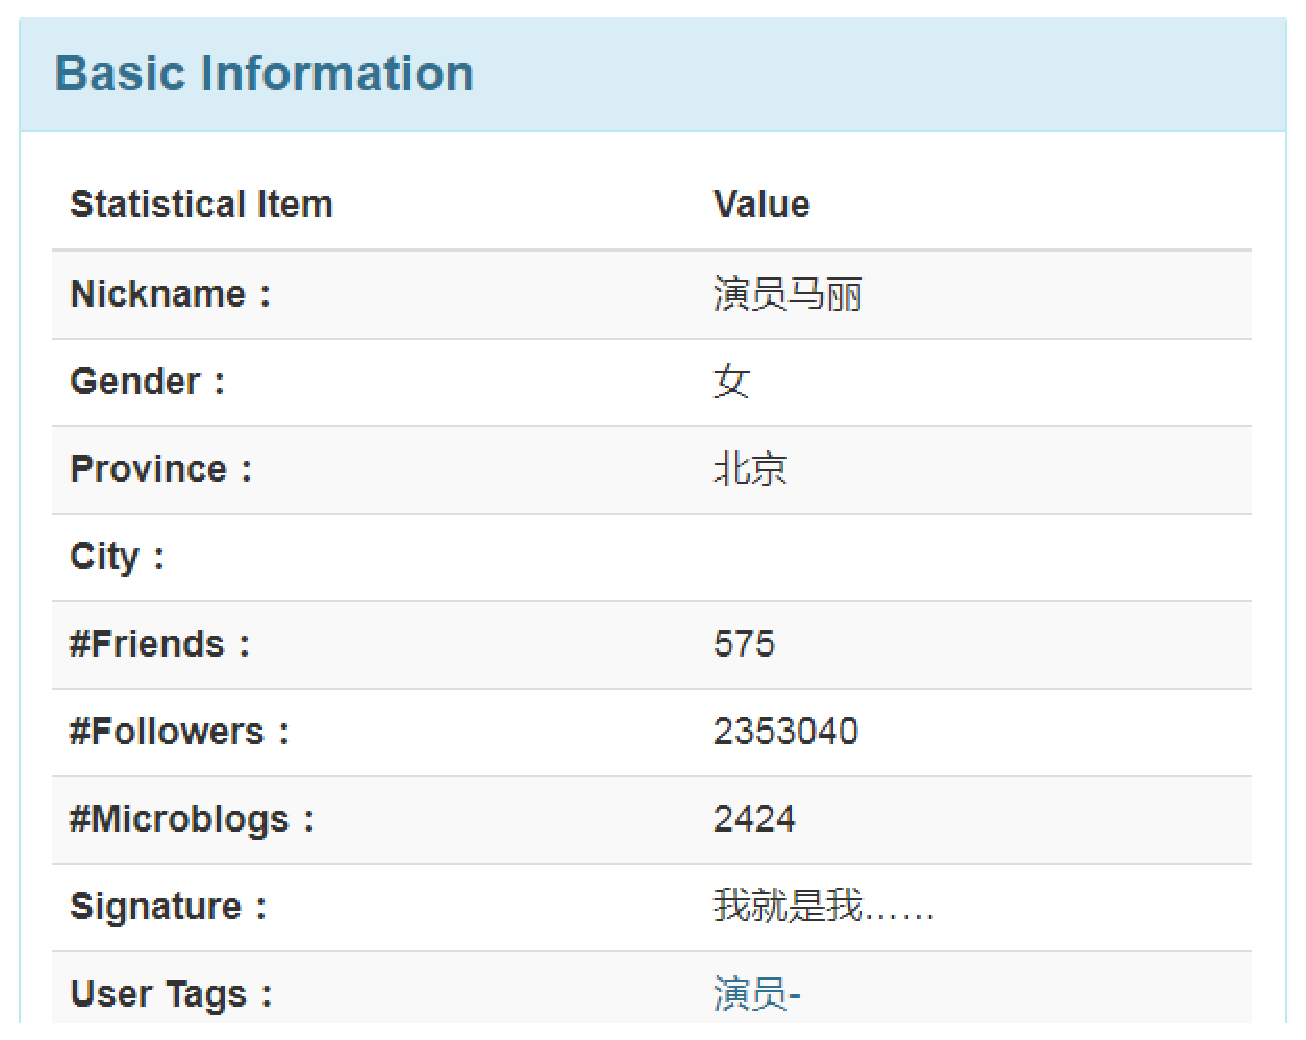
\includegraphics[width=0.23\textwidth]{IMAGE/features/userFeatures/1.eps}}
  \subfigure[]{
      \label{fig:userFeatures:uf-2}
      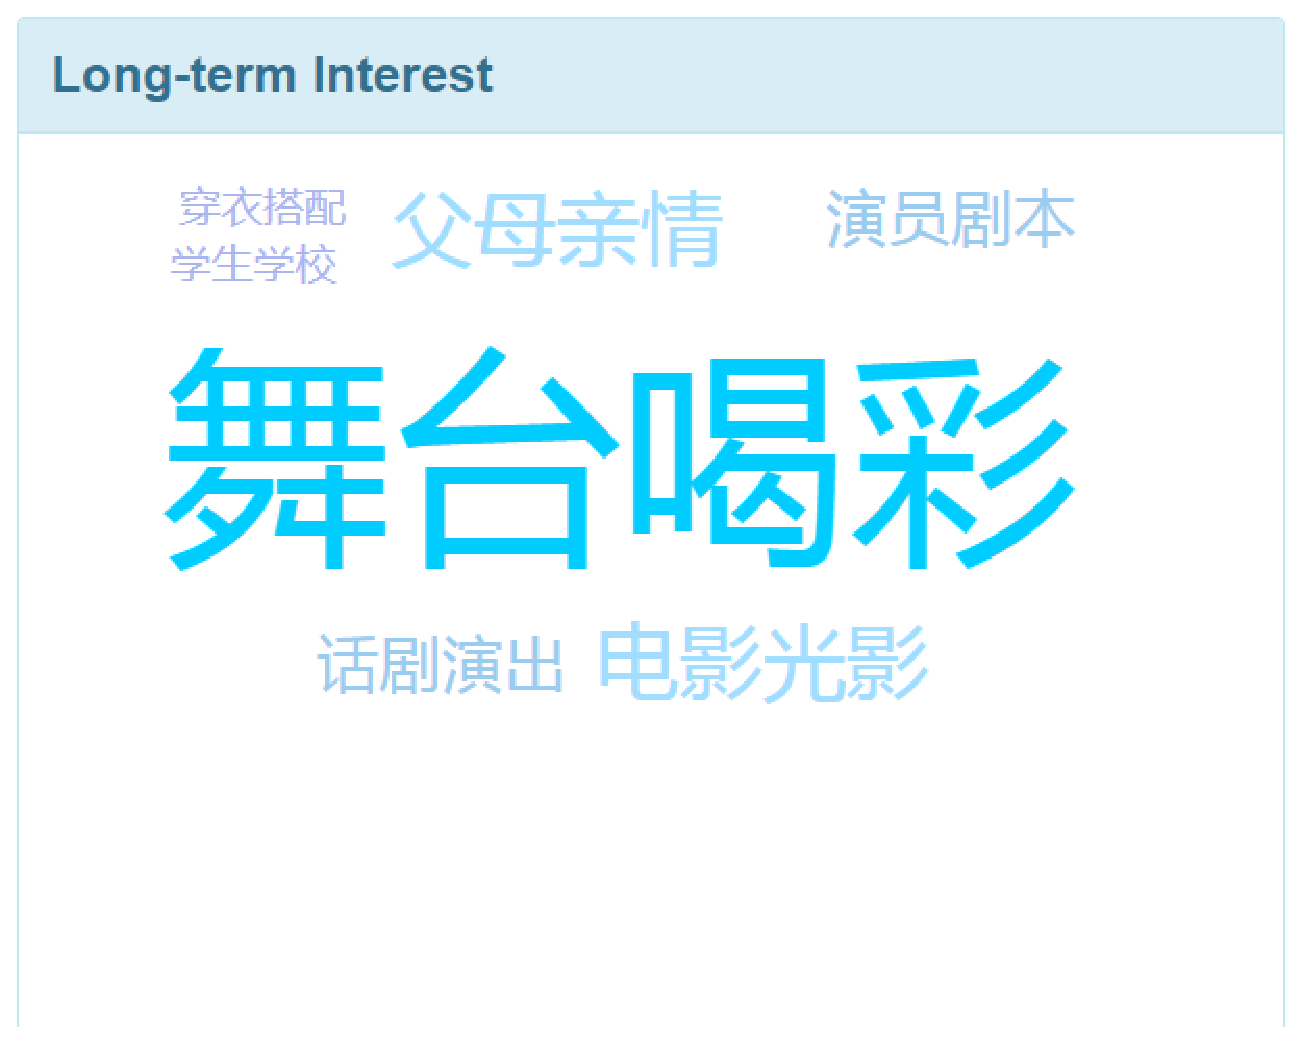
\includegraphics[width=0.23\textwidth]{IMAGE/features/userFeatures/2.eps}}
  \subfigure[]{
      \label{fig:userFeatures:uf-3}
      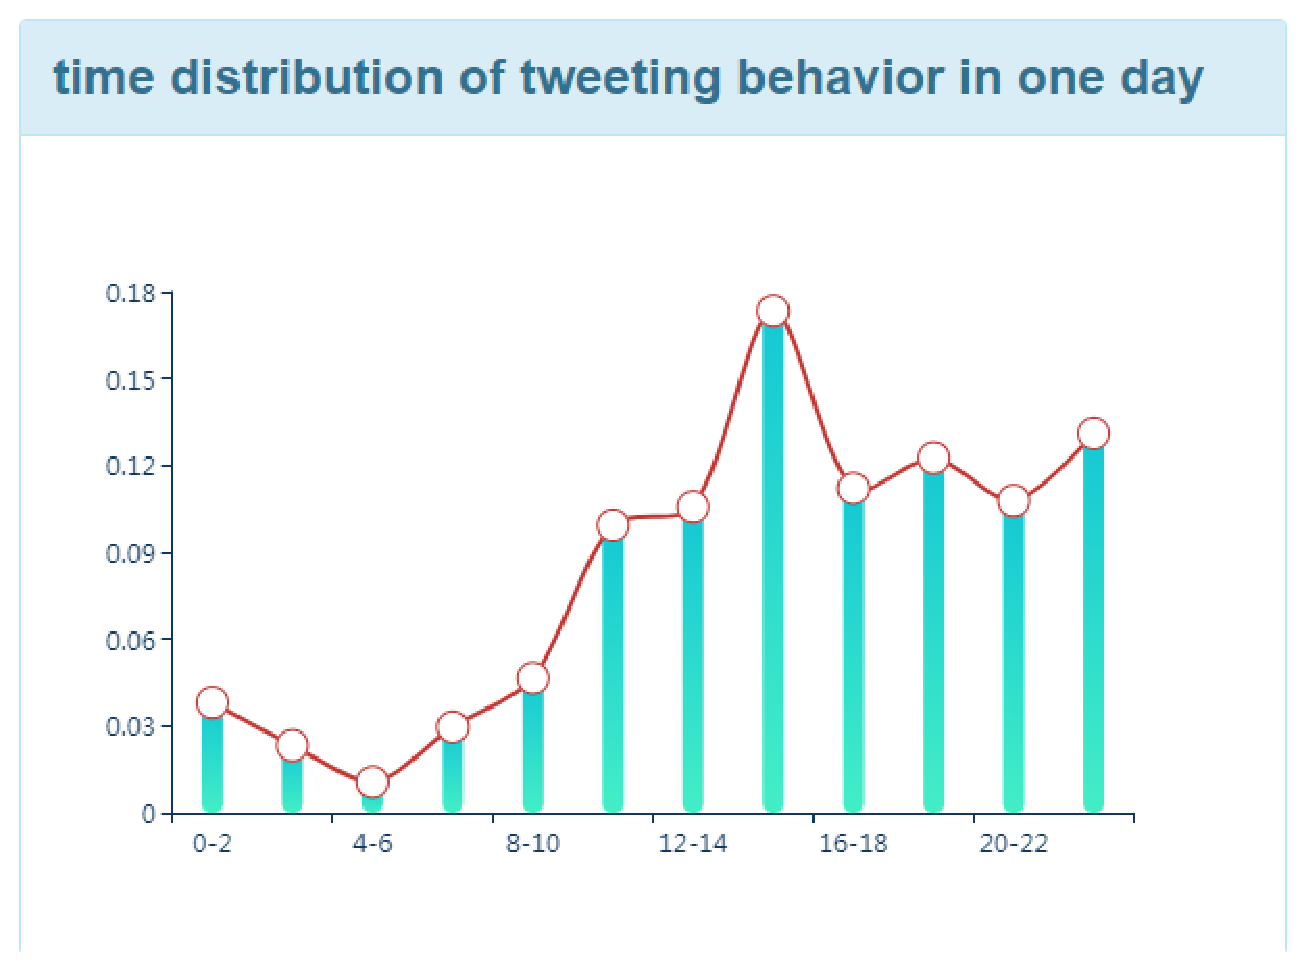
\includegraphics[width=0.23\textwidth]{IMAGE/features/userFeatures/3.eps}}
  \subfigure[]{
      \label{fig:userFeatures:uf-4}
      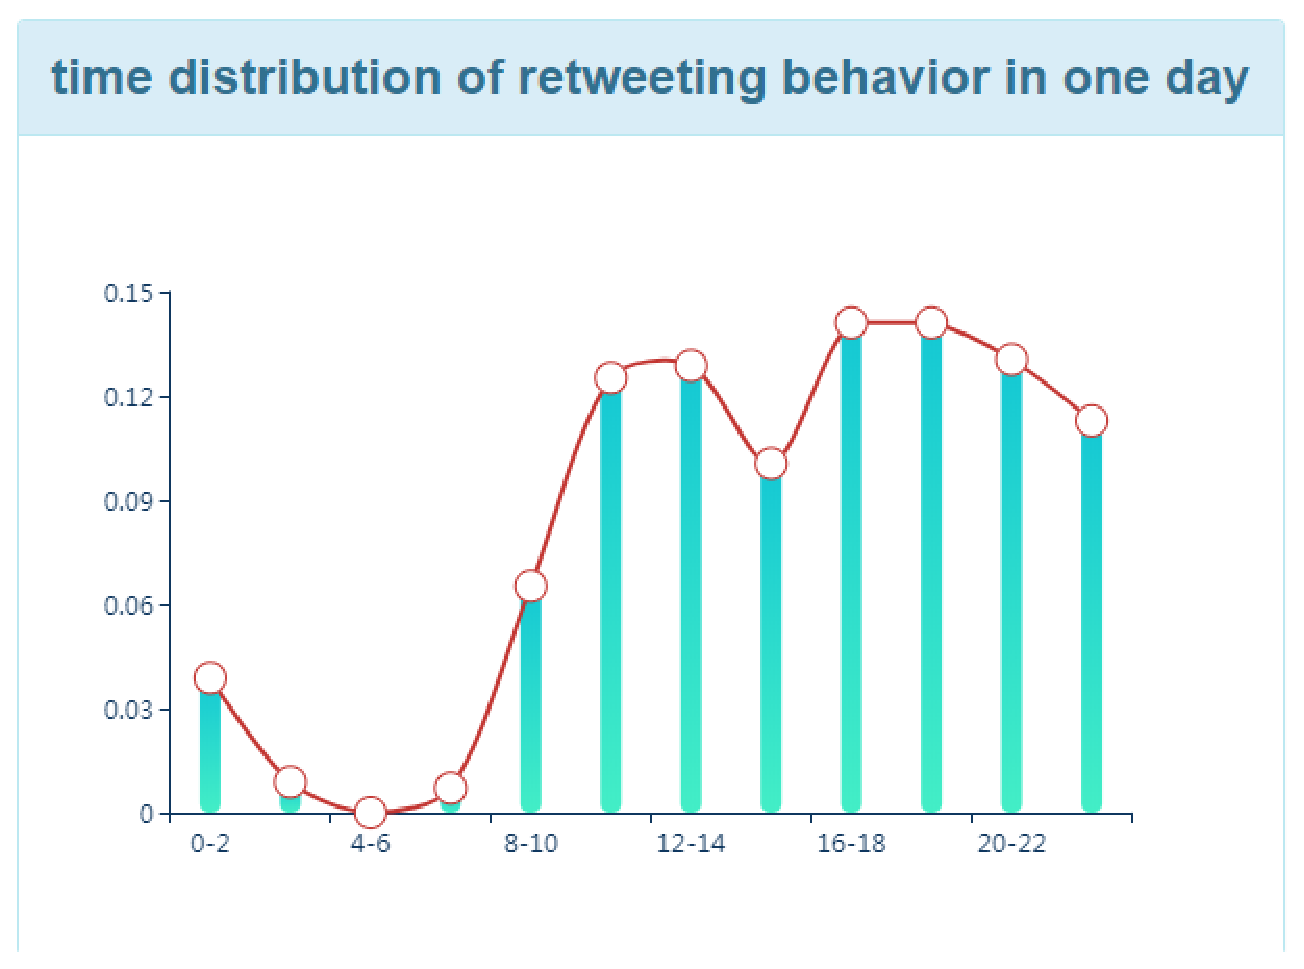
\includegraphics[width=0.23\textwidth]{IMAGE/features/userFeatures/4.eps}}
  \subfigure[]{
      \label{fig:userFeatures:uf-5}
      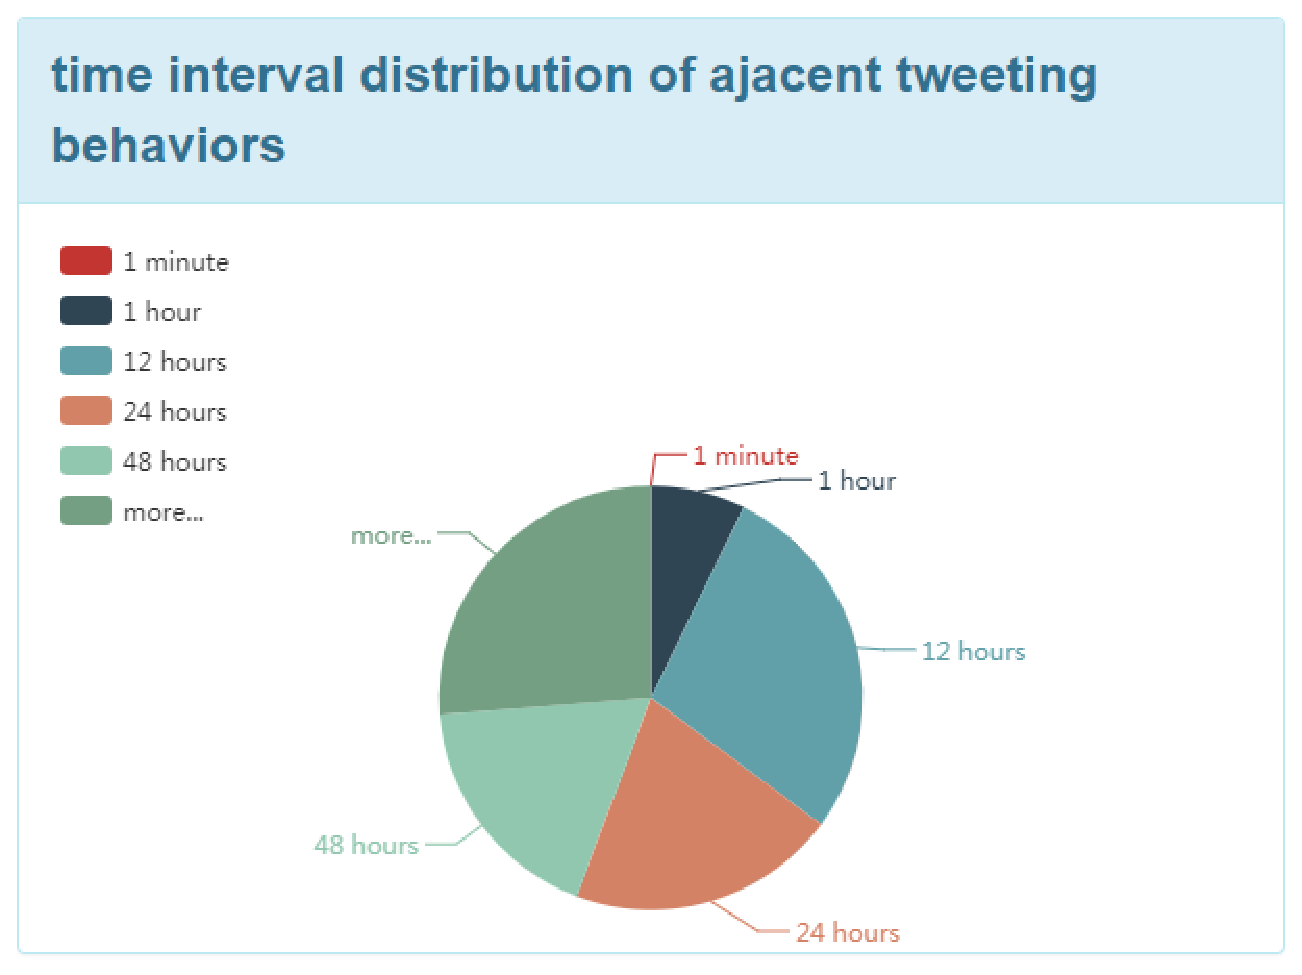
\includegraphics[width=0.23\textwidth]{IMAGE/features/userFeatures/5.eps}}
  \subfigure[]{
      \label{fig:userFeatures:uf-6}
      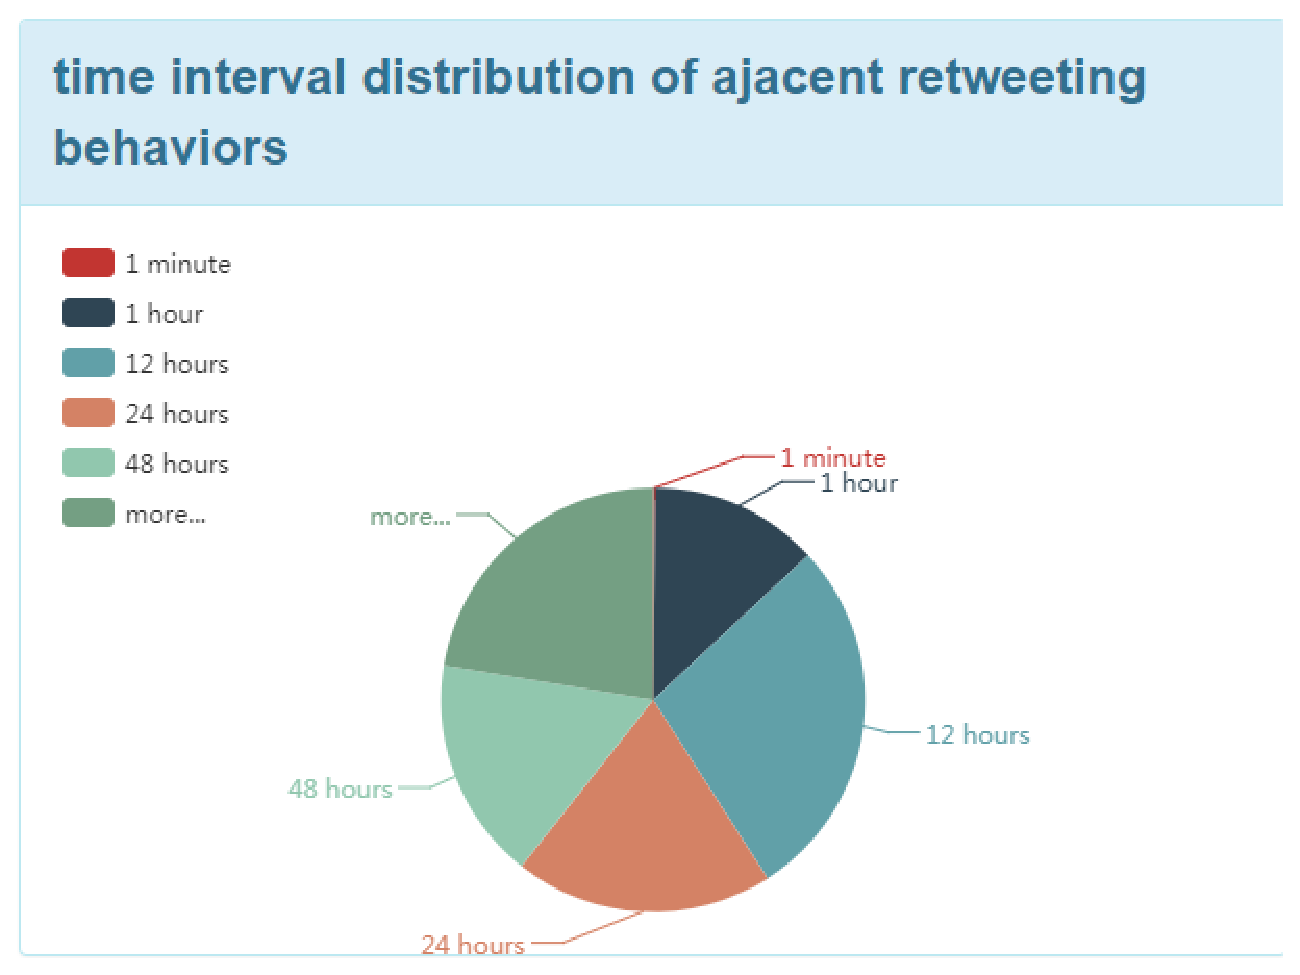
\includegraphics[width=0.23\textwidth]{IMAGE/features/userFeatures/6.eps}}
  \subfigure[]{
      \label{fig:userFeatures:uf-7}
      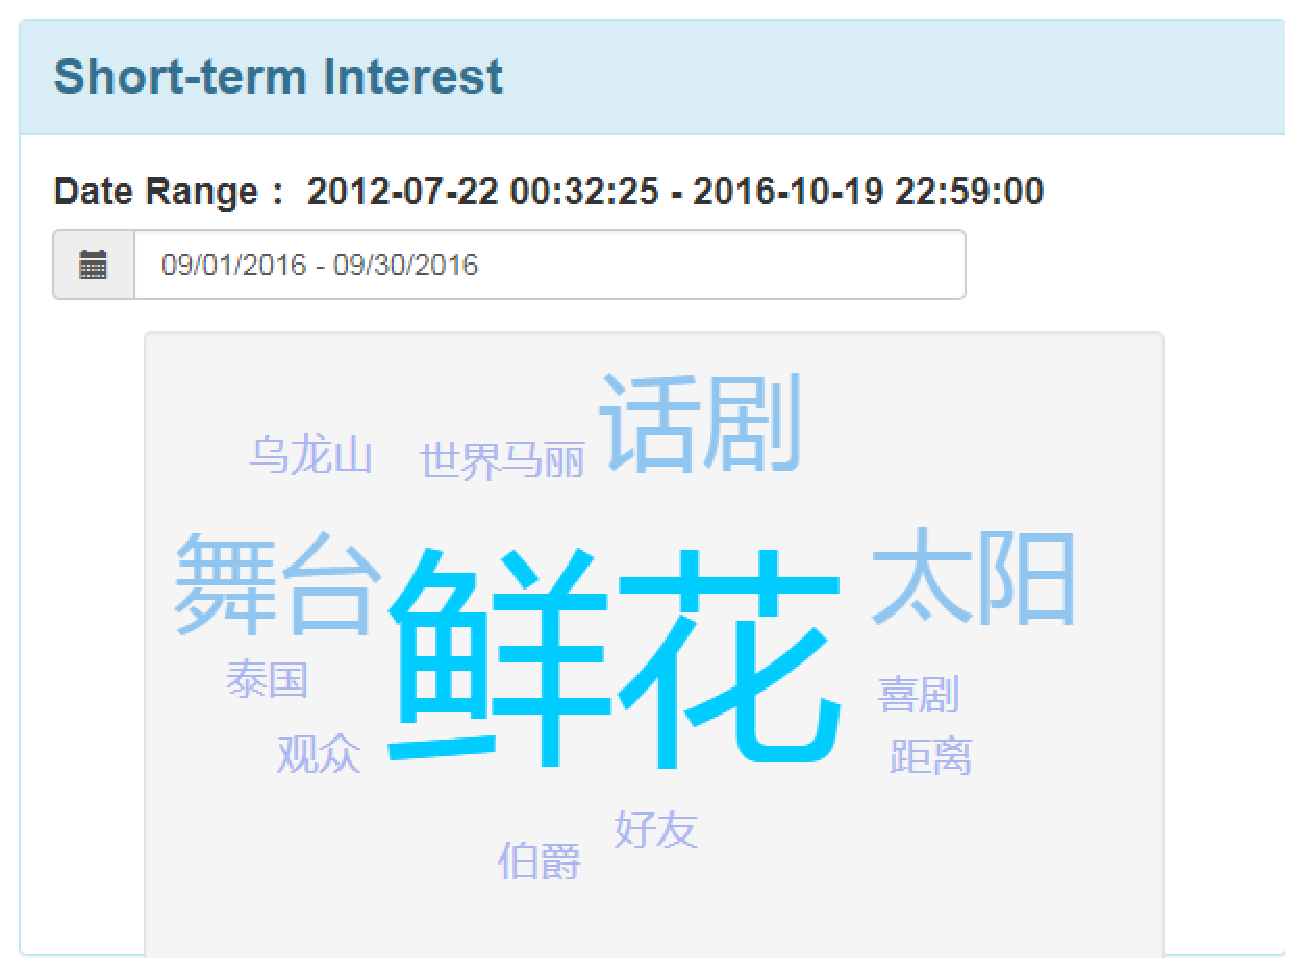
\includegraphics[width=0.23\textwidth]{IMAGE/features/userFeatures/7.eps}}
  \subfigure[]{
      \label{fig:userFeatures:uf-8}
      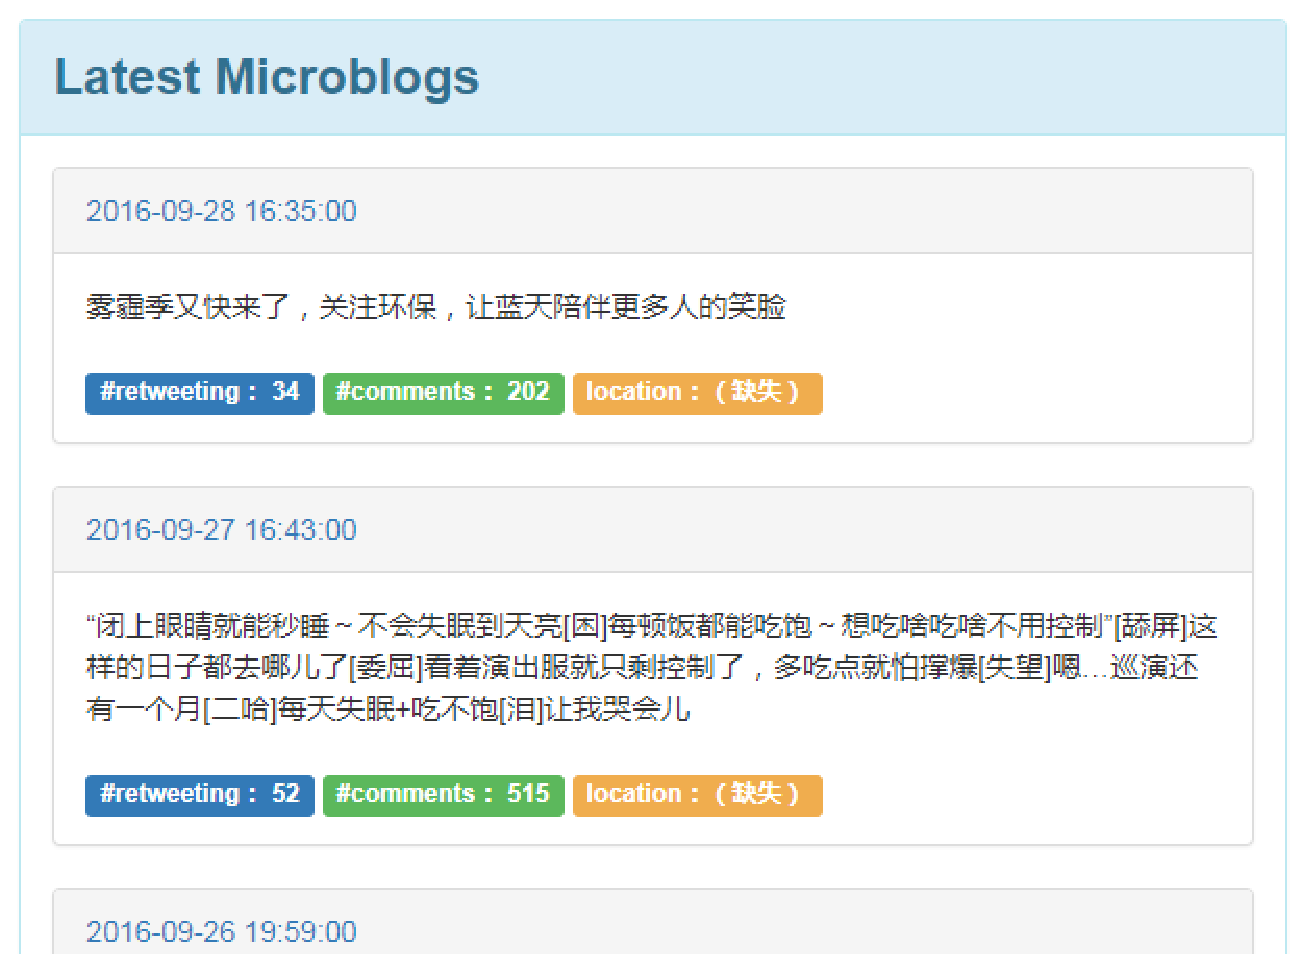
\includegraphics[width=0.24\textwidth]{IMAGE/features/userFeatures/8.eps}}
  \caption{Visualization for User Features.}
  \label{fig:userFeatures} %% label for entire figure
  \vspace{-2ex}
\end{figure*}


\stitle{Exp-4: Case Study for Feature Extraction}
In this test, we show the results of our demo system for user features extraction.
%
Considering the huge amount of users, we carefully selected one typical user for analysis.
Here we chose Mary (a famous drama and movie actress in China) as an example.

The feature extraction result for Mary is depicted in Fig.\ \ref{fig:userFeatures}.
Then we can see the basic information of Mary in Fig.\ \ref{fig:userFeatures:uf-1}: her nickname is Actress Mary (��Ա����) and she is from Beijing (����).
Mary has more followers than followees.
The Sina Microblog tag she made for herself is ``actress'' (��Ա).
As to the long-term interest, she is interested with stage performance (��̨����), drama (�������),film (��Ӱ��Ӱ) and so on as shown in Fig.\ \ref{fig:userFeatures:uf-2}, which is consistent with her tag.
The probability distribution of tweeting and retweeting indicates that she is more active at night than daytime as shown in Fig.\ \ref{fig:userFeatures:uf-3} and \ref{fig:userFeatures:uf-4}.
According to Fig.\ \ref{fig:userFeatures:uf-5} and \ref{fig:userFeatures:uf-6}, the interval between her two tweeted/retweeted microblogs is mostly within 48 hours, showing she is an active user.
Mary's short-term interest, e.g. from 09/01/2016 to 09/30/2016, is shown in Fig.\ \ref{fig:userFeatures:uf-7}, which indicates she had been busy with promoting the drama ``Earl of Oolong Mountain'' (����ɽ����). So the results are in line with expectations, as drama (����) and stage (��̨) in Fig.\ \ref{fig:userFeatures:uf-7}.



To conclude, by modeling user behaviors over groups instead of a single model for all users such as LRC-BQ, we improve the average accuracy over LRC-BQ by 6\%. What deserves to be mentioned is that the performance of LRC-BQ is also improved significantly by user clustering.

%
\section*{Appendix: Extra Experiments}
\label{sec:appendix}

%\subsection{Case Study for Feature Extraction}
\begin{figure*}
  \centering
  \subfigure[]{
  \label{fig:subfig1:fig11}
      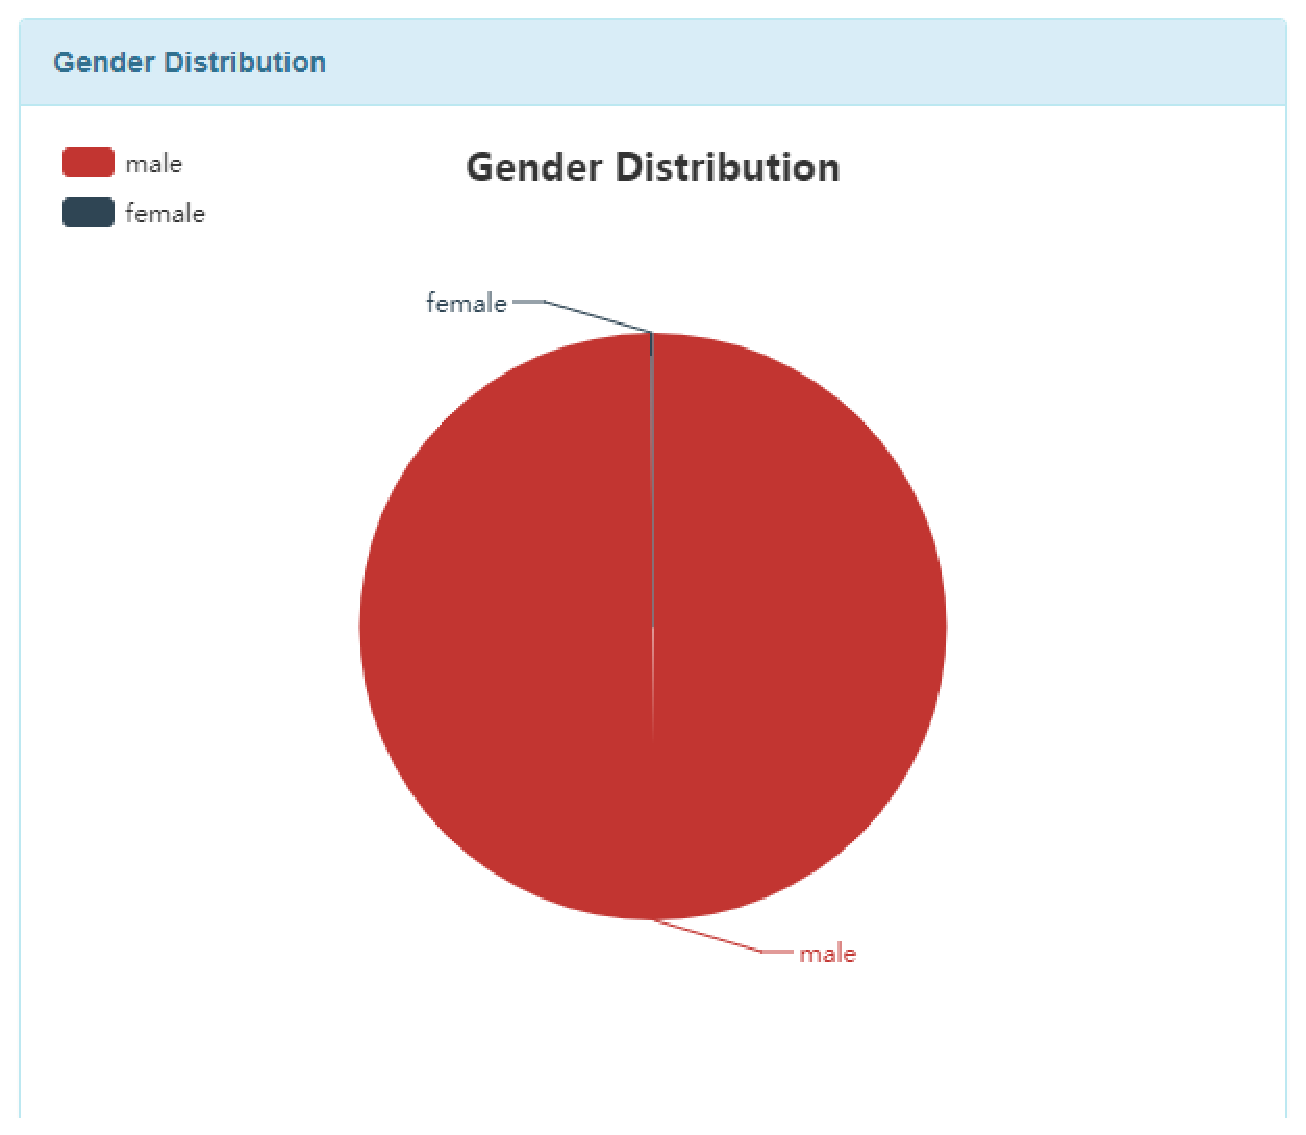
\includegraphics[width=0.23\textwidth]{IMAGE/group-images/11.eps}}
  \subfigure[]{
  \label{fig:subfig1:fig12}
      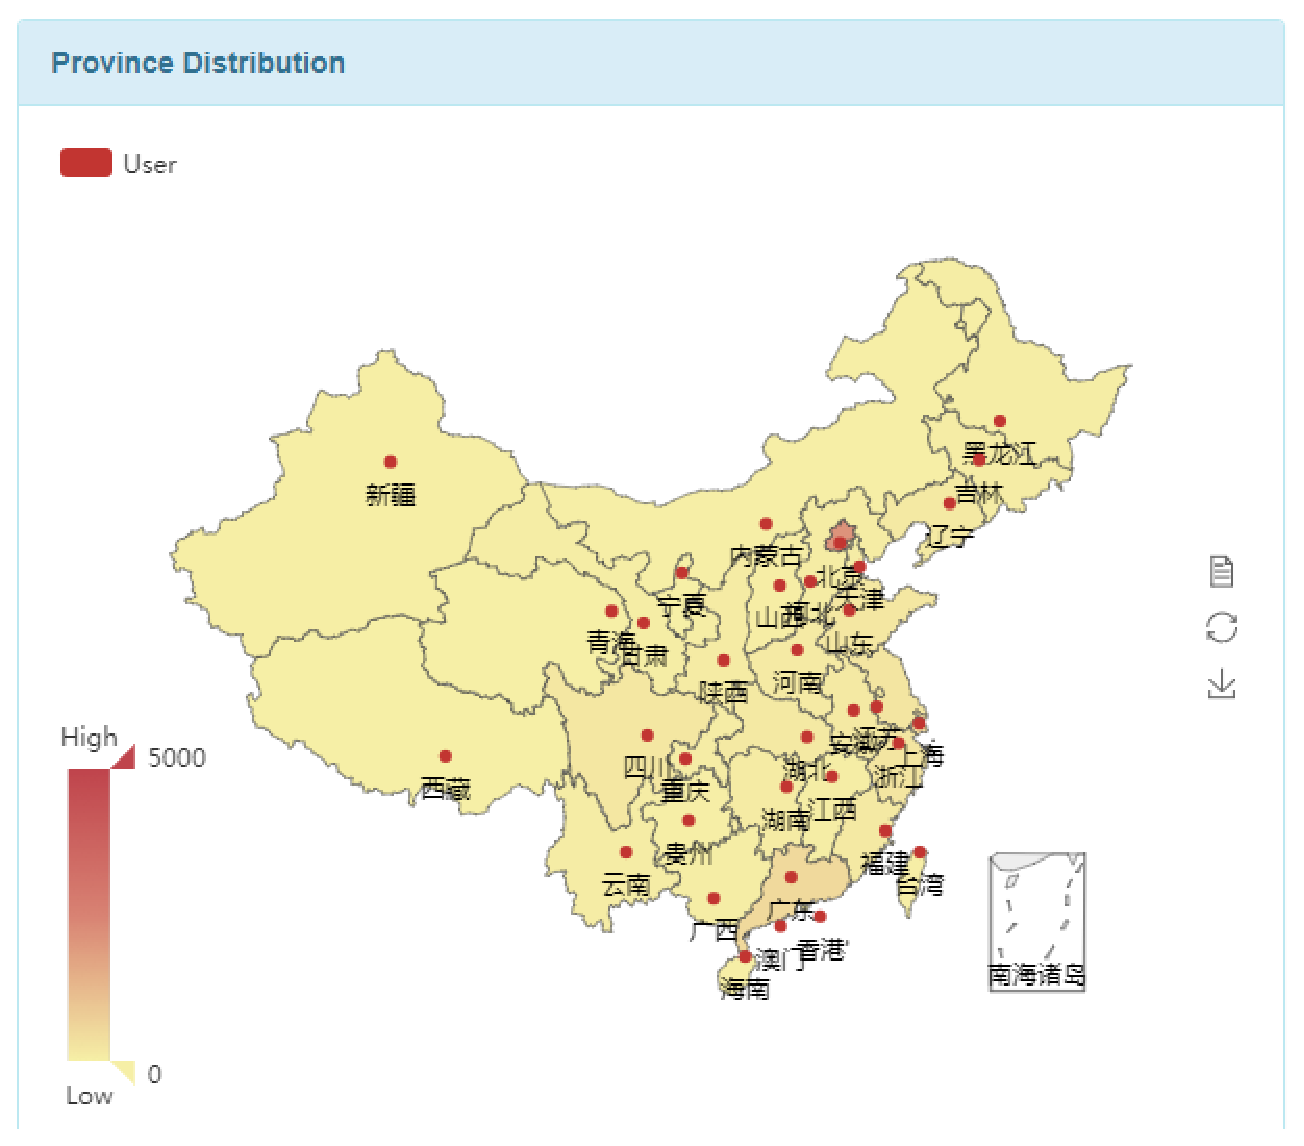
\includegraphics[width=0.23\textwidth]{IMAGE/group-images/12.eps}}
  \subfigure[]{
  \label{fig:subfig1:fig13}
      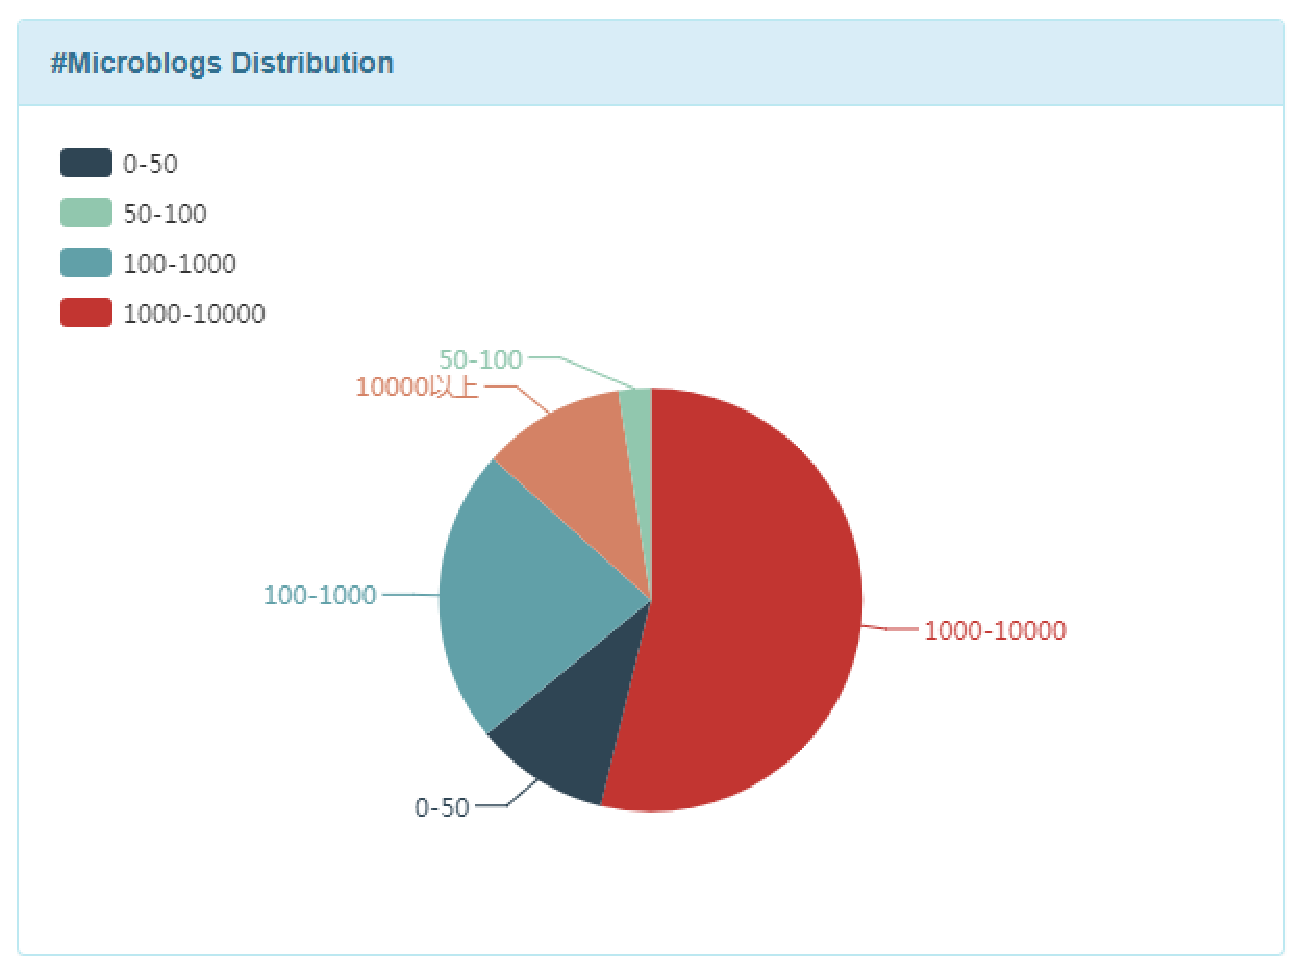
\includegraphics[width=0.23\textwidth]{IMAGE/group-images/13.eps}}
  \subfigure[]{
  \label{fig:subfig1:fig14}
      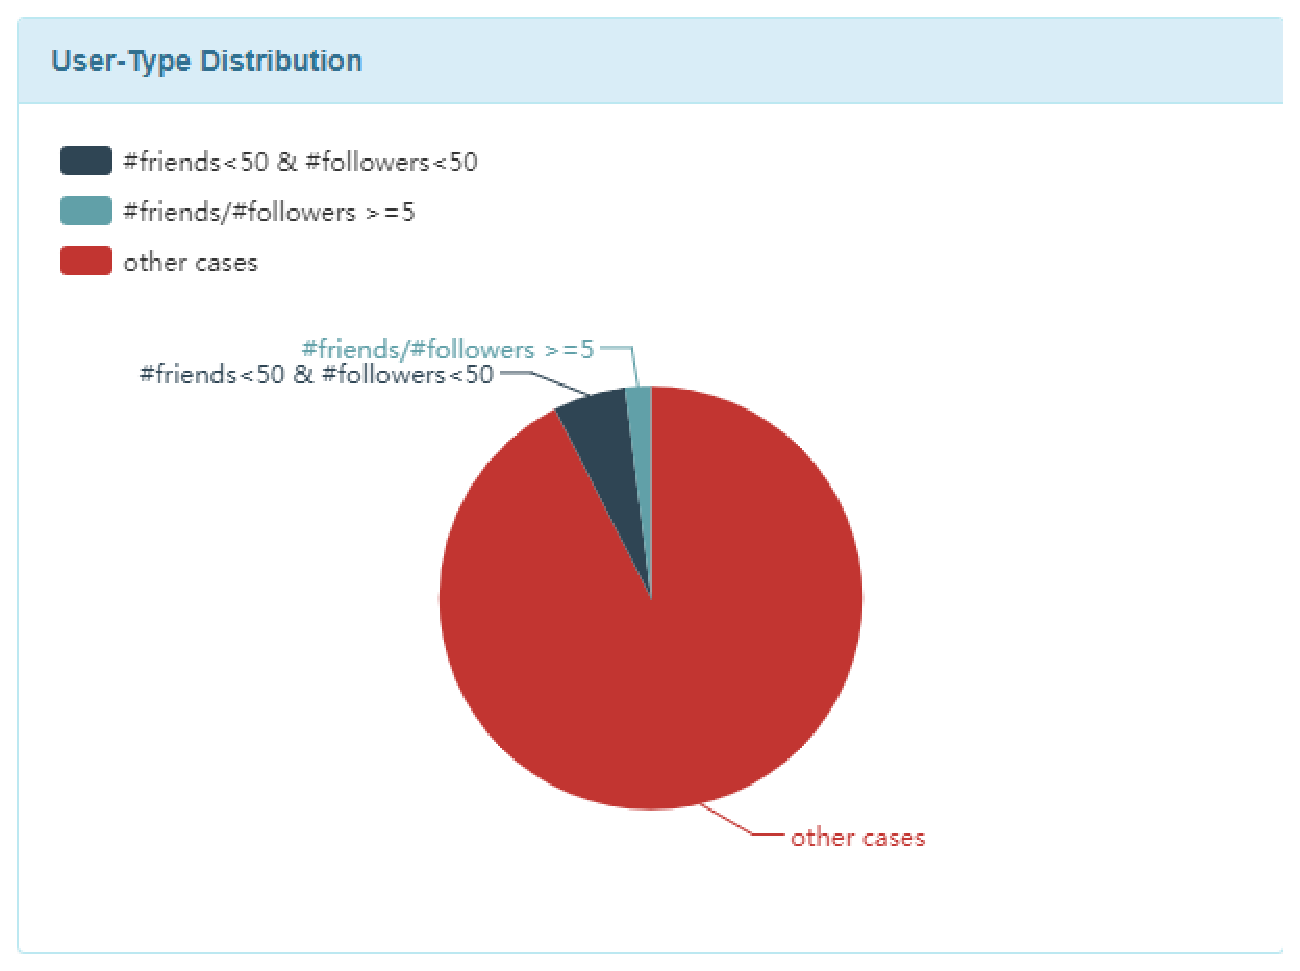
\includegraphics[width=0.23\textwidth]{IMAGE/group-images/14.eps}}
  \subfigure[]{
  \label{fig:subfig1:fig15}
      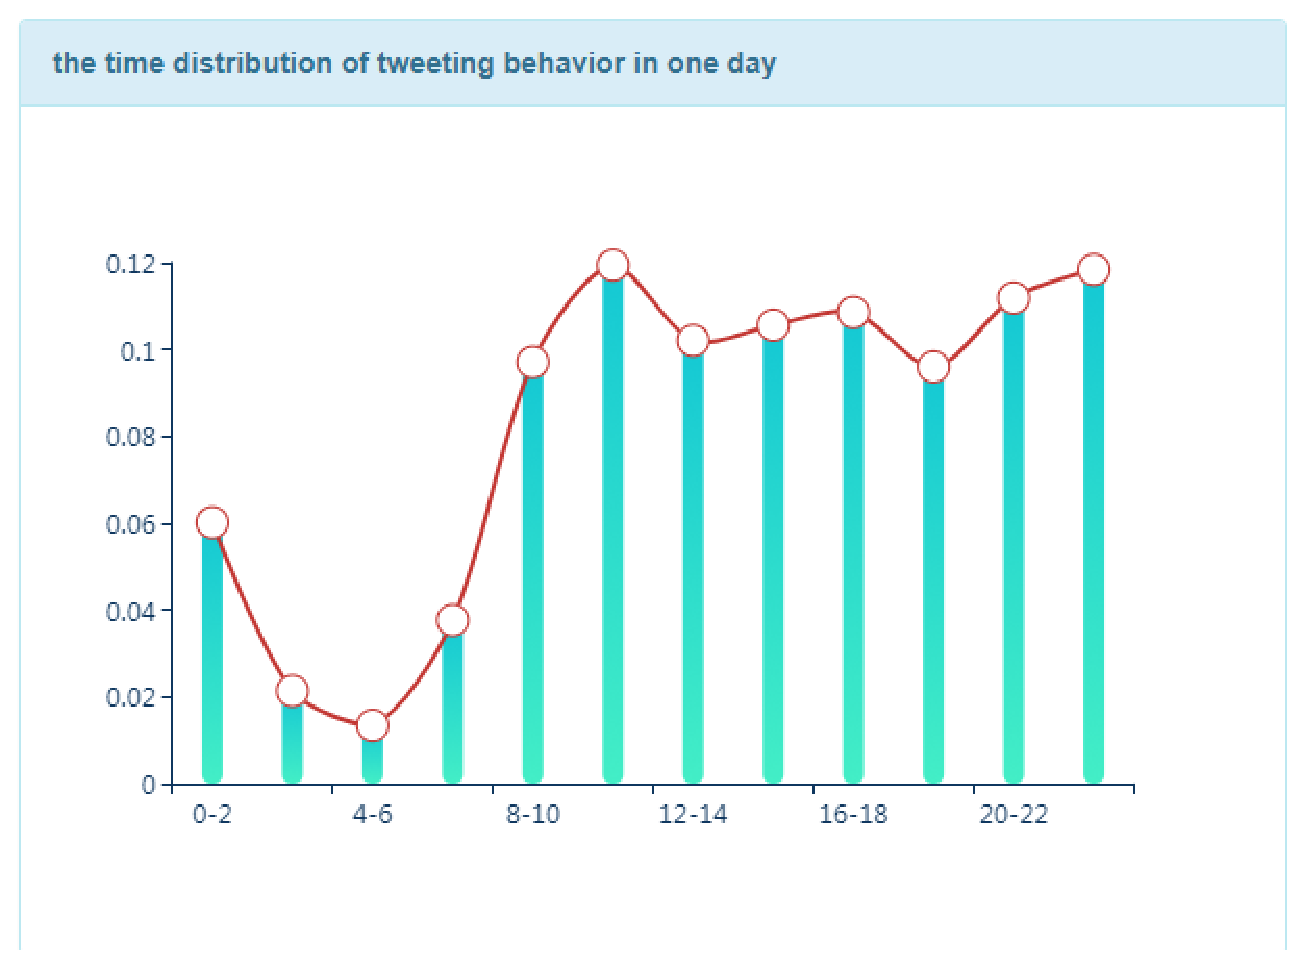
\includegraphics[width=0.23\textwidth]{IMAGE/group-images/15.eps}}
  \subfigure[]{
  \label{fig:subfig1:fig16}
      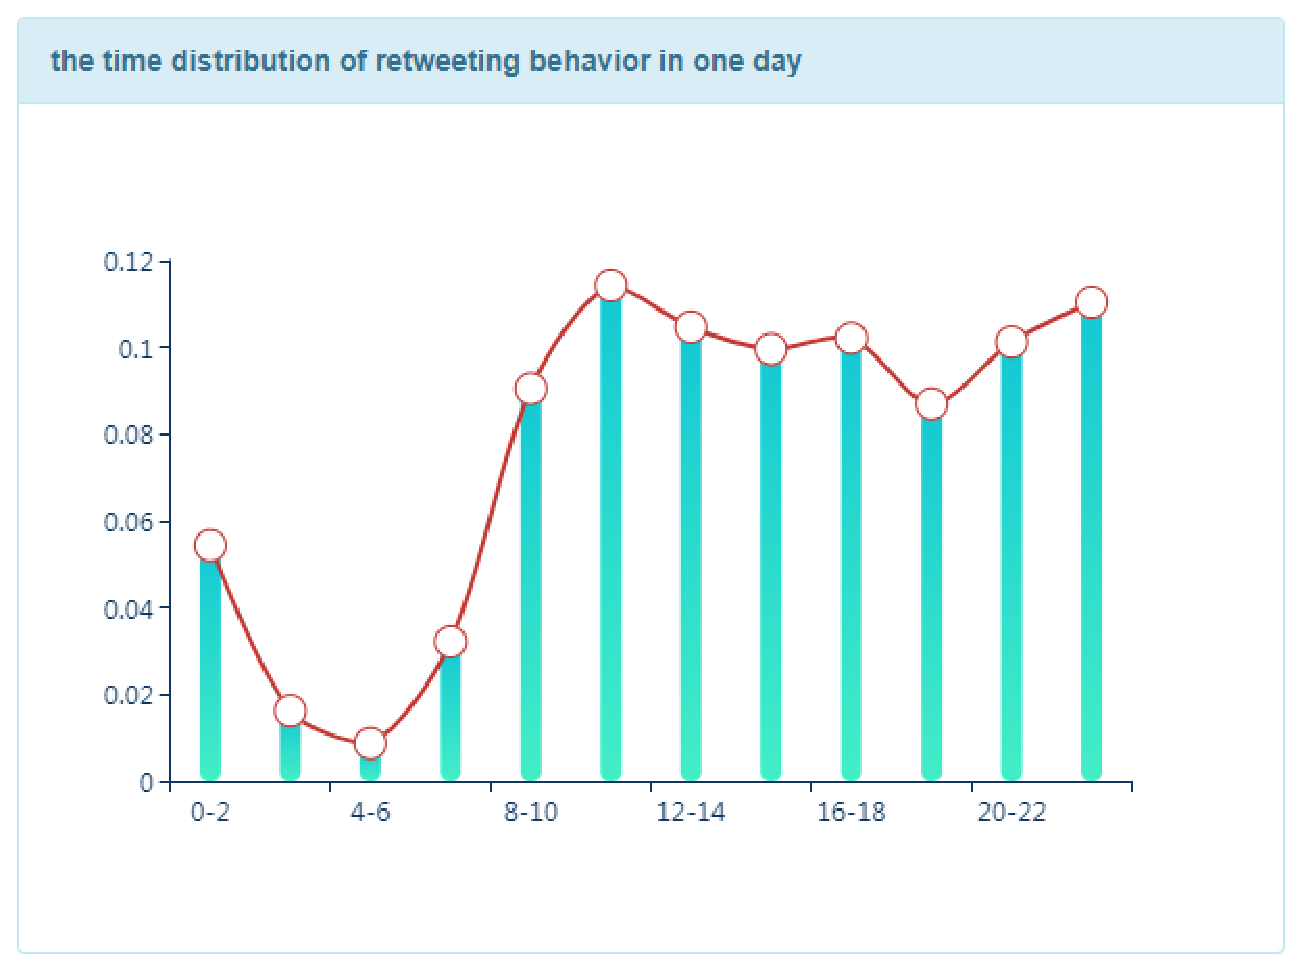
\includegraphics[width=0.23\textwidth]{IMAGE/group-images/16.eps}}
  \subfigure[]{
  \label{fig:subfig1:fig17}
      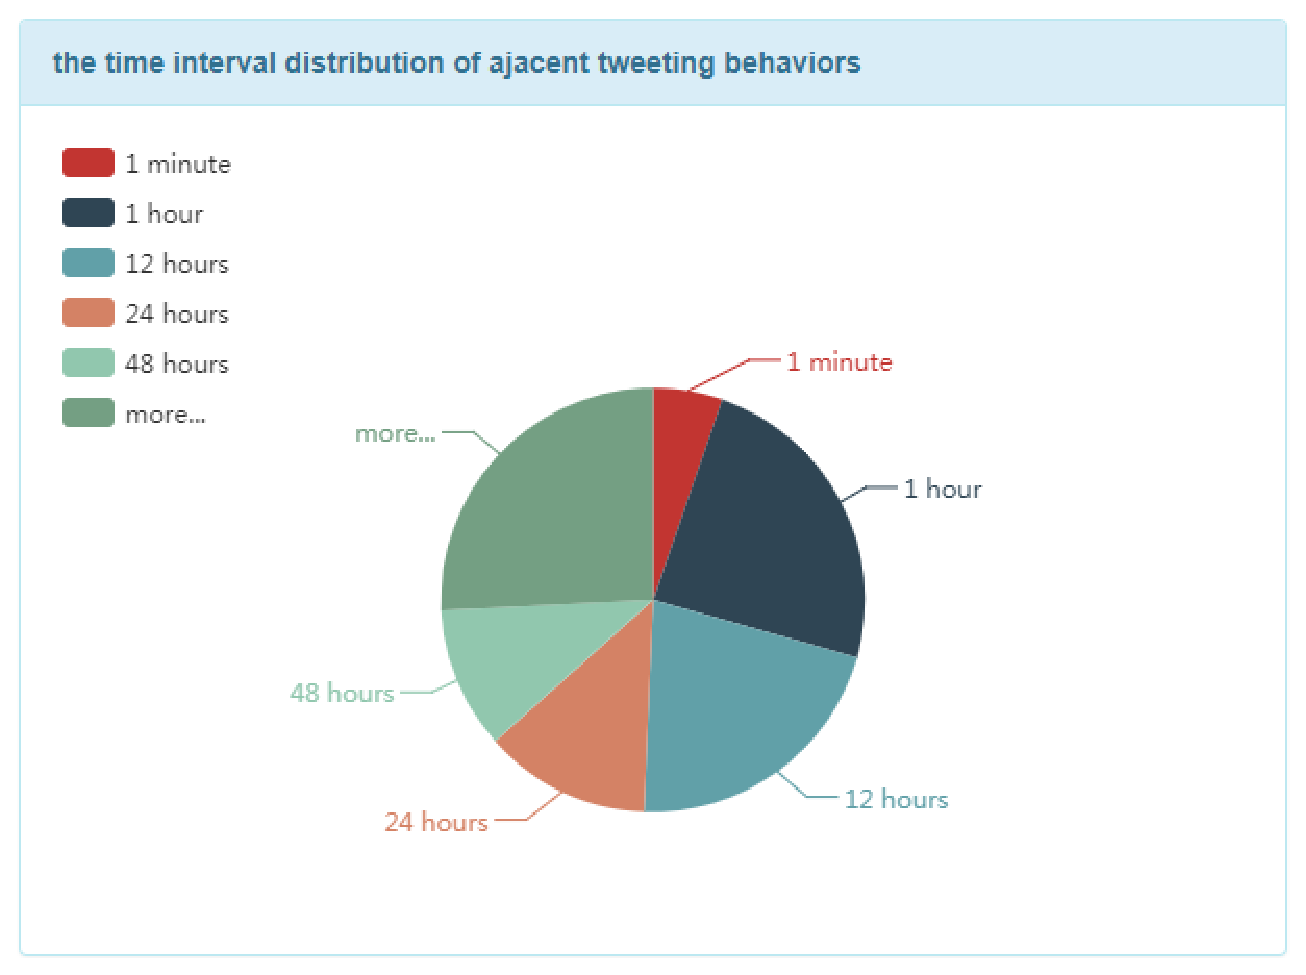
\includegraphics[width=0.23\textwidth]{IMAGE/group-images/17.eps}}
  \subfigure[]{
  \label{fig:subfig1:fig18}
      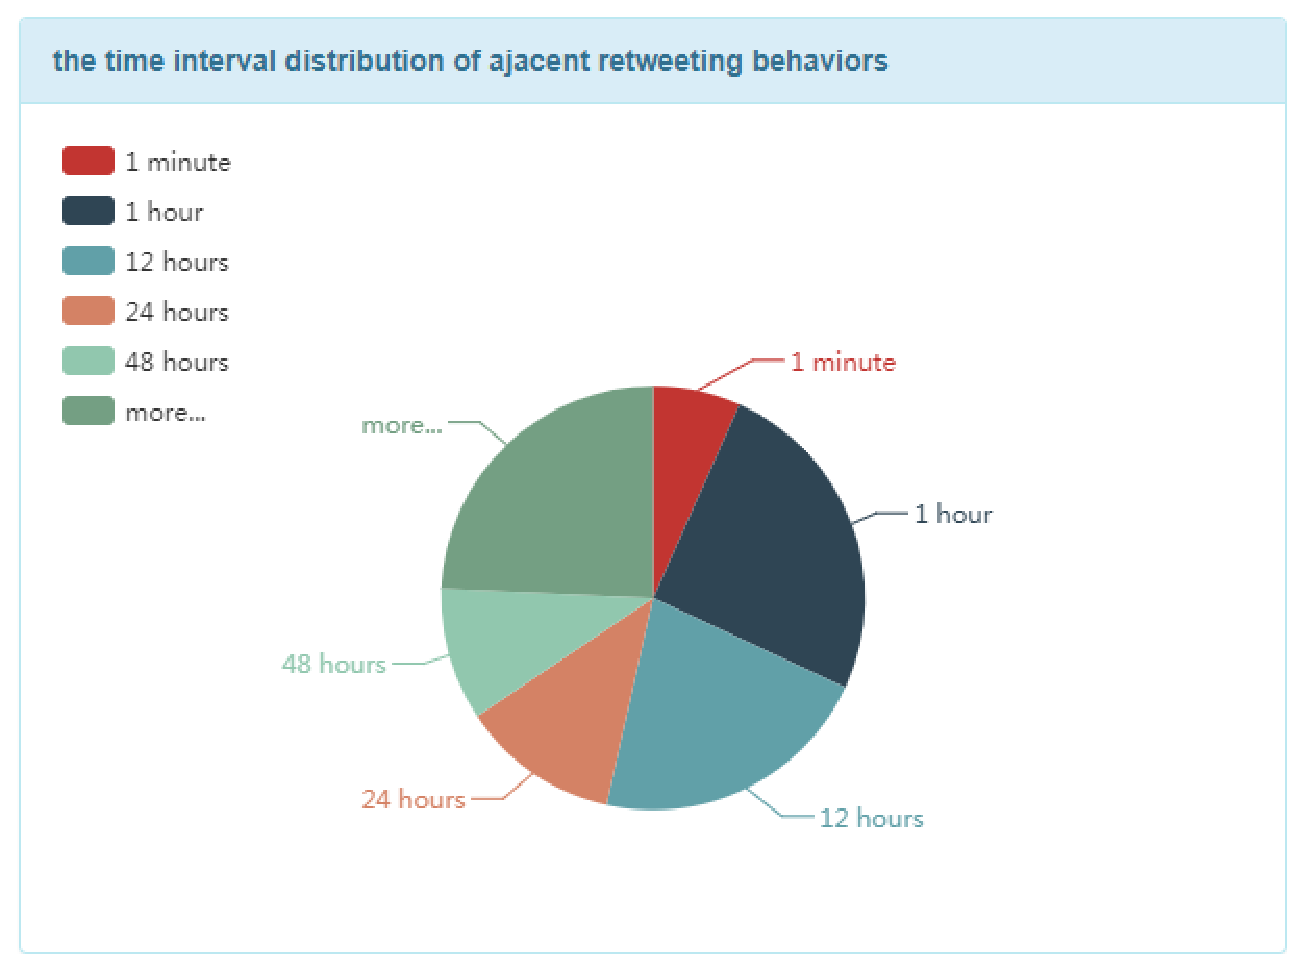
\includegraphics[width=0.23\textwidth]{IMAGE/group-images/18.eps}}
  \subfigure[]{
  \label{fig:subfig1:fig19}
      
\includegraphics[width=0.23\textwidth]{IMAGE/group-images/19.eps}}
  \caption{The Statistics of User Group One}
  \label{fig:subfig1} %% label for entire figure
\end{figure*}

\subsection*{Exp-5: Case Study for User Clustering}

In this section, we show the results of our system \sys{} for User Clustering. We carefully analyzed the statistical information of four groups obtained from user clustering.

\stab(1) Most users of group one are male (as shown in Sub-Fig. \ref{fig:subfig1:fig11}), and Sub-Fig. \ref{fig:subfig1:fig12} shows that they are mainly in Beijing(����). The amount of their followees is mostly similar as their followers (as shown in Sub-Fig. \ref{fig:subfig1:fig14}). The most active time of this group is mainly between 10 am and 12 am (as shown in Sub-Fig. \ref{fig:subfig1:fig15} and \ref{fig:subfig1:fig16}).

\stab(2) Mostly users of group two are  female (as shown in Sub-Fig. \ref{fig:subfig2:fig21}) and are also mainly in Beijing (����) (shown as Sub-Fig. \ref{fig:subfig2:fig22}). Similar to group one, most of them have followees close to followers (as shown in Sub-Fig. \ref{fig:subfig2:fig24}). The most active time of this group is mainly between 10 pm and 12 pm (as shown in Sub-Fig. \ref{fig:subfig2:fig25} and \ref{fig:subfig2:fig26}).

\stab(3) Most users of group three are male (as shown in Sub-Fig. \ref{fig:subfig3:fig31}). They come from a wide range of provinces (as shown in Sub-Fig. \ref{fig:subfig3:fig32}). Most of them have number of followers far more than followees (as shown in Sub-Fig. \ref{fig:subfig3:fig34}). The most active time of this group is mainly in 10-12 am and 10-12 pm (as shown in Sub-Fig. \ref{fig:subfig3:fig35} and \ref{fig:subfig3:fig36}).

\stab(4) Most users of group four are female (as shown in Sub-Fig. \ref{fig:subfig4:fig41}), and they come from a wide range of provinces just as group three (as shown in Sub-Fig. \ref{fig:subfig4:fig42}). Most of these users have the amount  of followers far more than followees (as shown in Sub-Fig. \ref{fig:subfig4:fig44}). And the most active time of these users is mainly between 10 pm and 12 pm (as shown in Sub-Fig. \ref{fig:subfig4:fig45} and \ref{fig:subfig4:fig46}).

According to Sub-Figs. \ref{fig:subfig1:fig13}, \ref{fig:subfig2:fig23}, \ref{fig:subfig3:fig33} and \ref{fig:subfig4:fig43},
the number distribution of microblogs for four groups is similar with each other.
We visualize each group's long-term interest expressed as words cloud (shown in Sub-Figs. \ref{fig:subfig1:fig19}, \ref{fig:subfig2:fig29}, \ref{fig:subfig3:fig39} and \ref{fig:subfig4:fig49}). As we can see, group one and group three have similar interests.



\begin{figure*}
  \centering
  \subfigure[]{
  \label{fig:subfig2:fig21}
      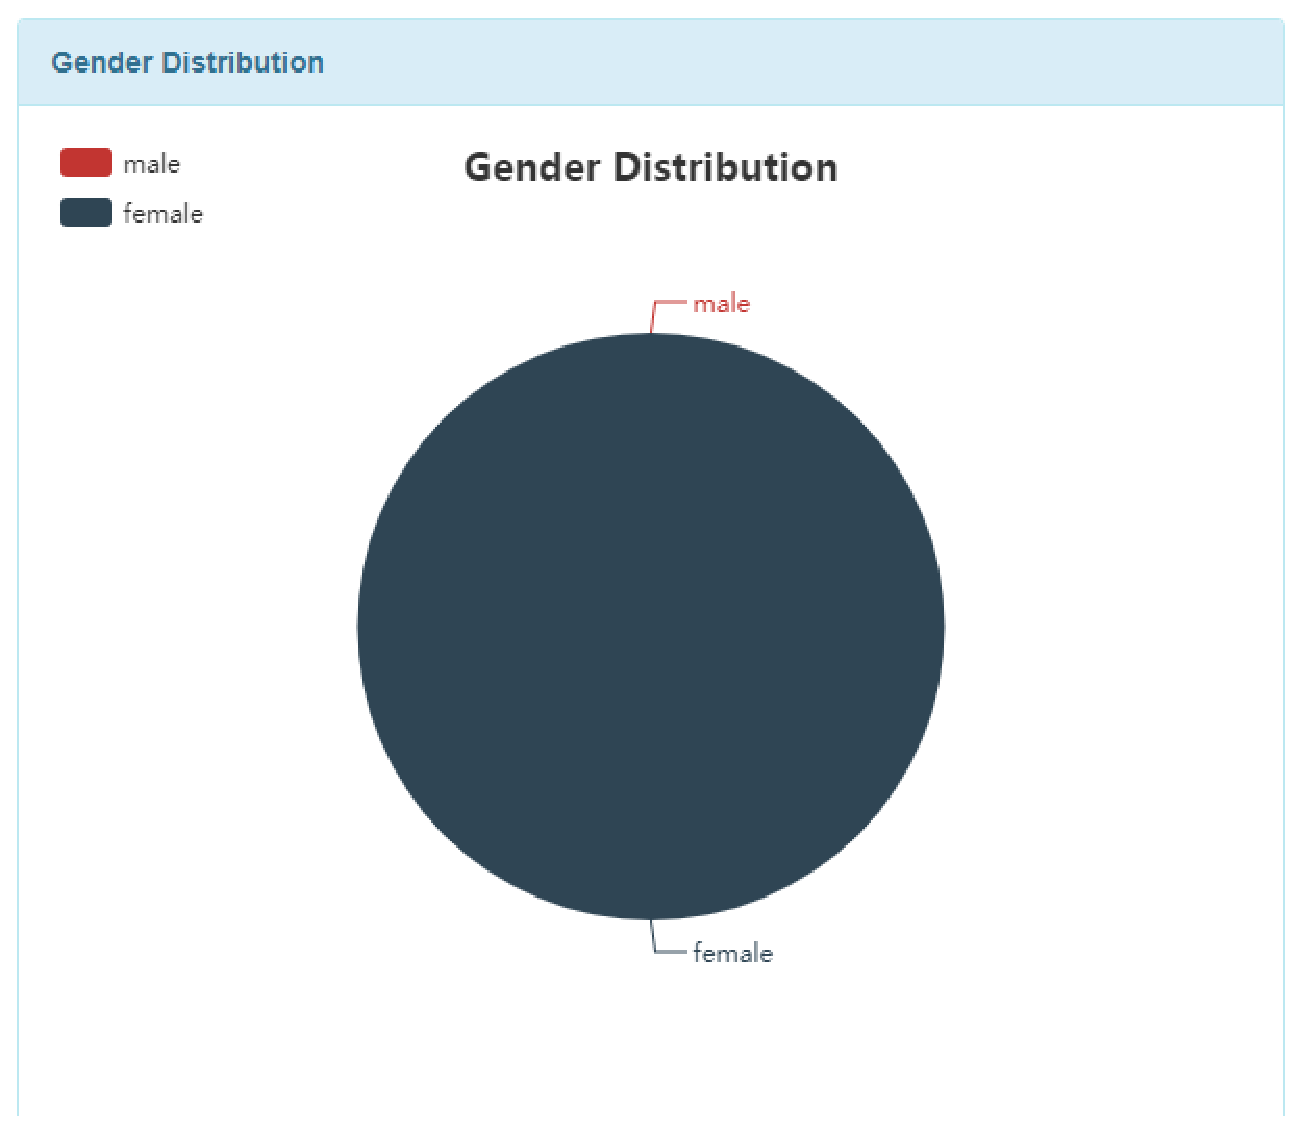
\includegraphics[width=0.23\textwidth]{IMAGE/group-images/21.eps}}
  \subfigure[]{
  \label{fig:subfig2:fig22}
      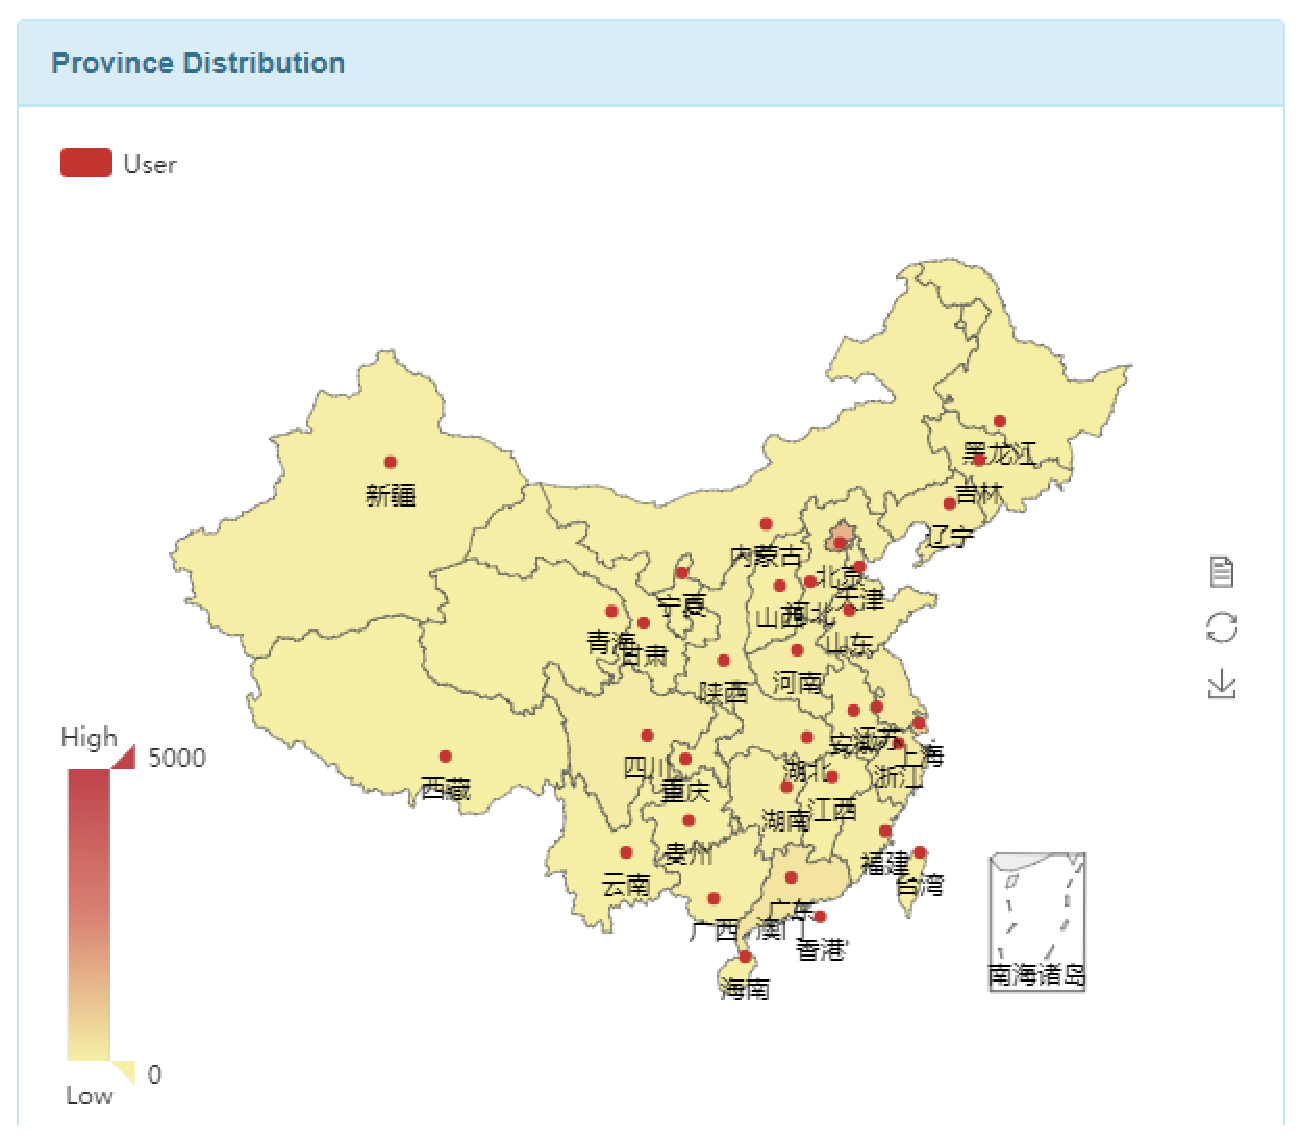
\includegraphics[width=0.23\textwidth]{IMAGE/group-images/22.eps}}
  \subfigure[]{
  \label{fig:subfig2:fig23}
      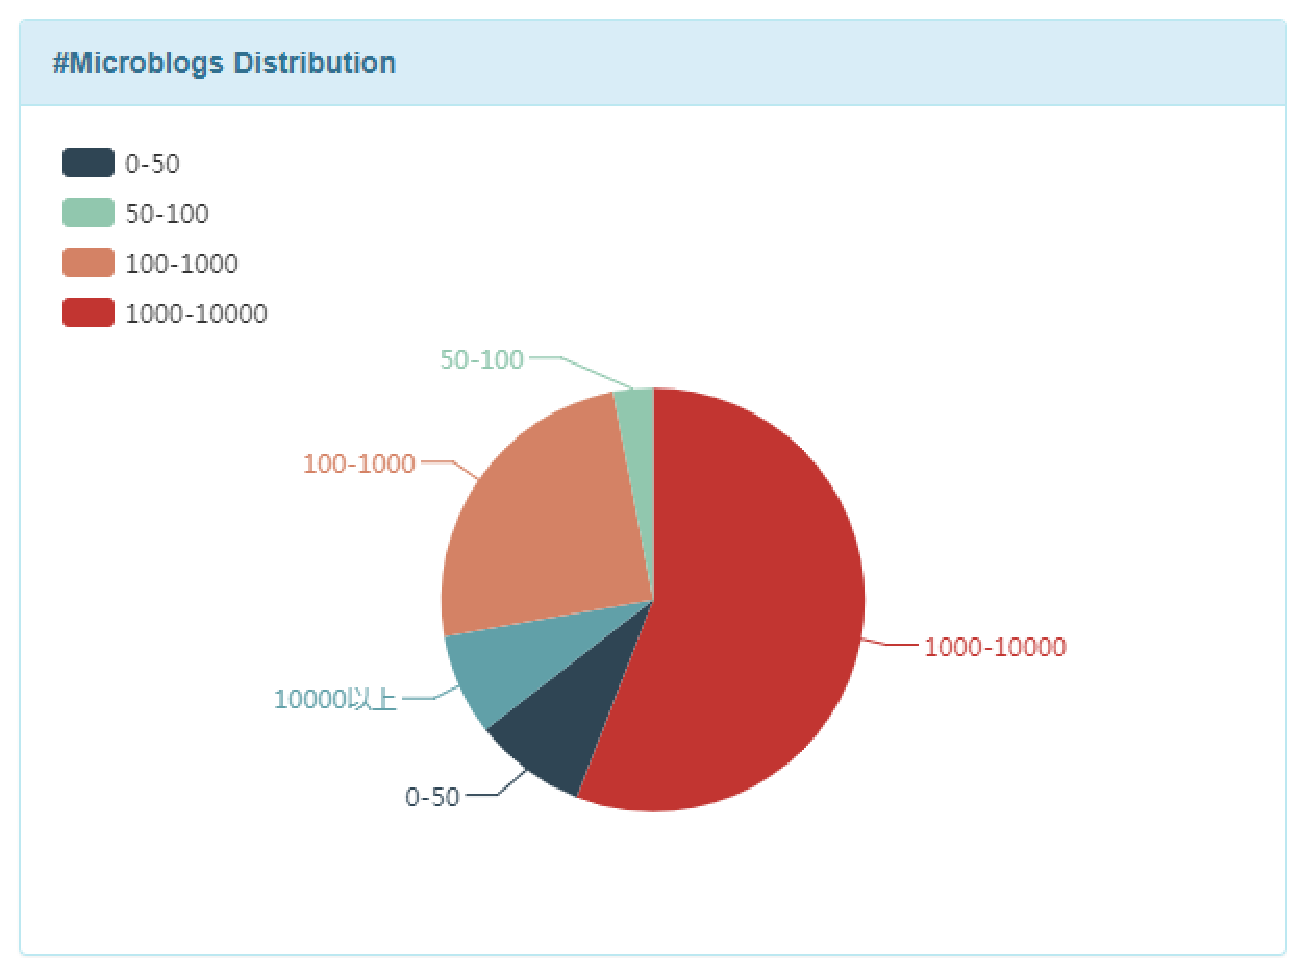
\includegraphics[width=0.23\textwidth]{IMAGE/group-images/23.eps}}
  \subfigure[]{
  \label{fig:subfig2:fig24}
      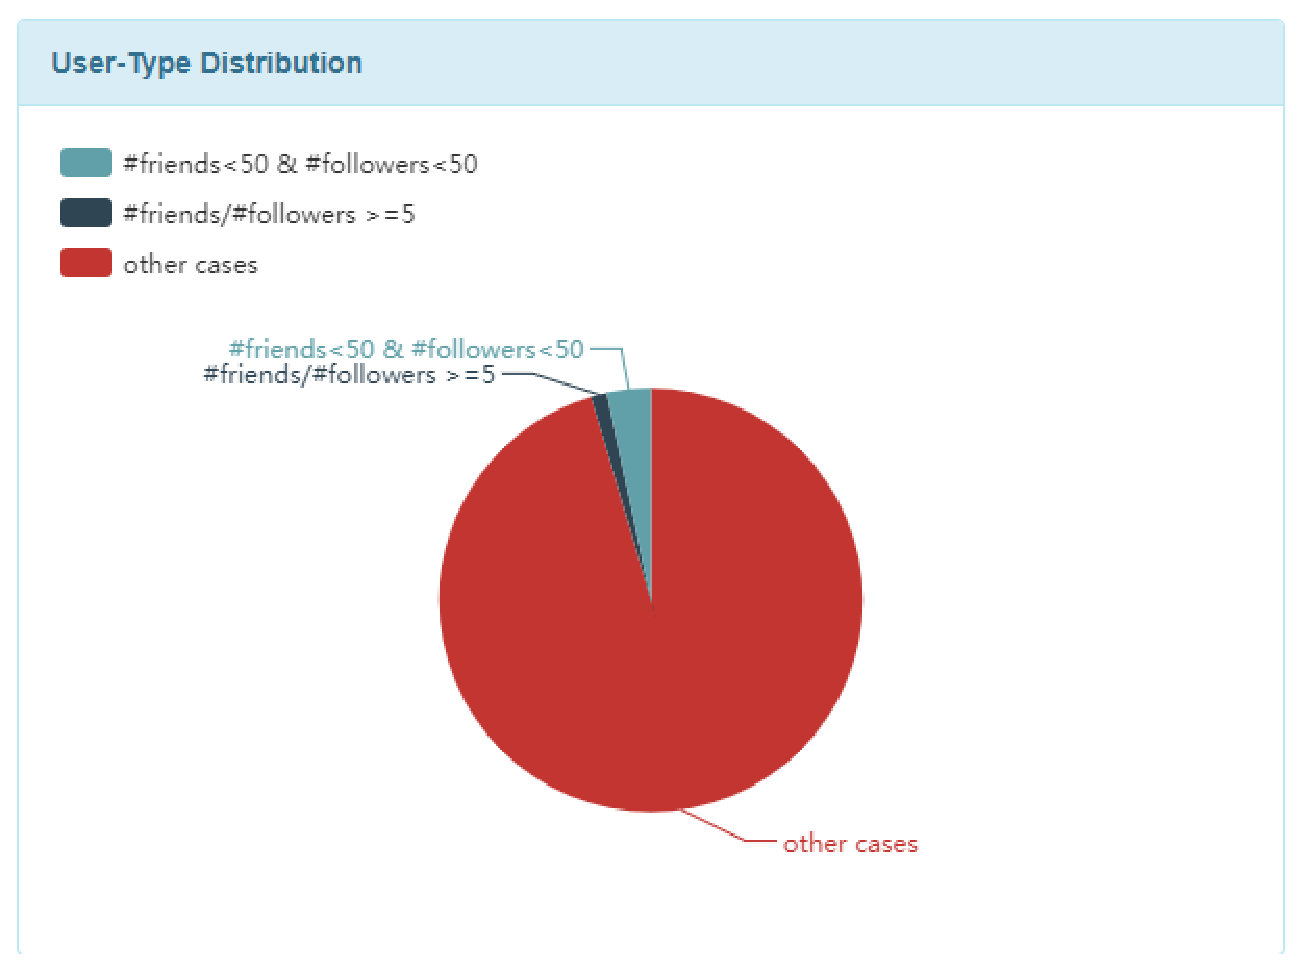
\includegraphics[width=0.23\textwidth]{IMAGE/group-images/24.eps}}
  \subfigure[]{
  \label{fig:subfig2:fig25}
      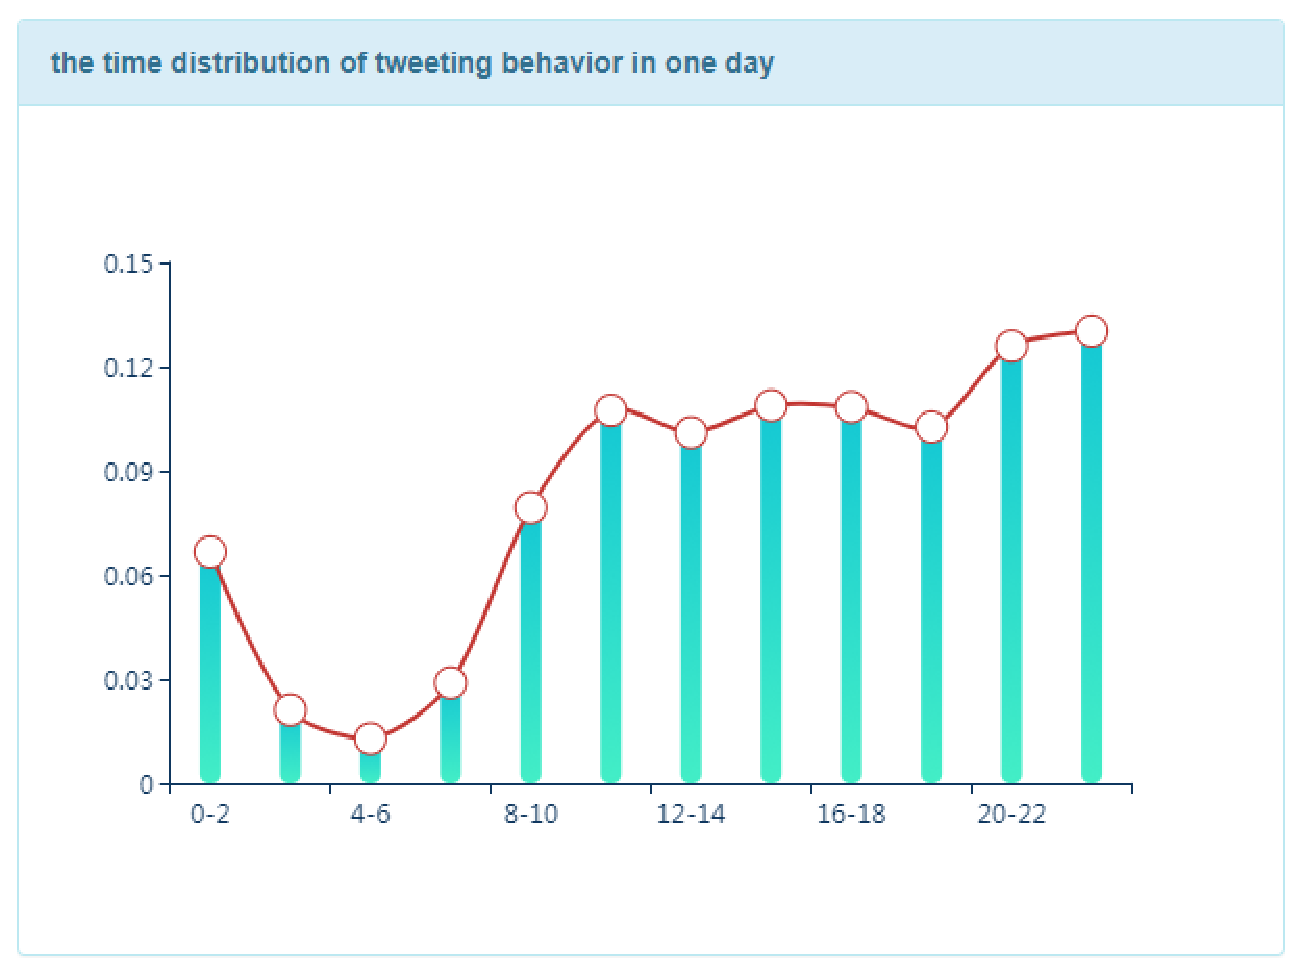
\includegraphics[width=0.23\textwidth]{IMAGE/group-images/25.eps}}
  \subfigure[]{
  \label{fig:subfig2:fig26}
      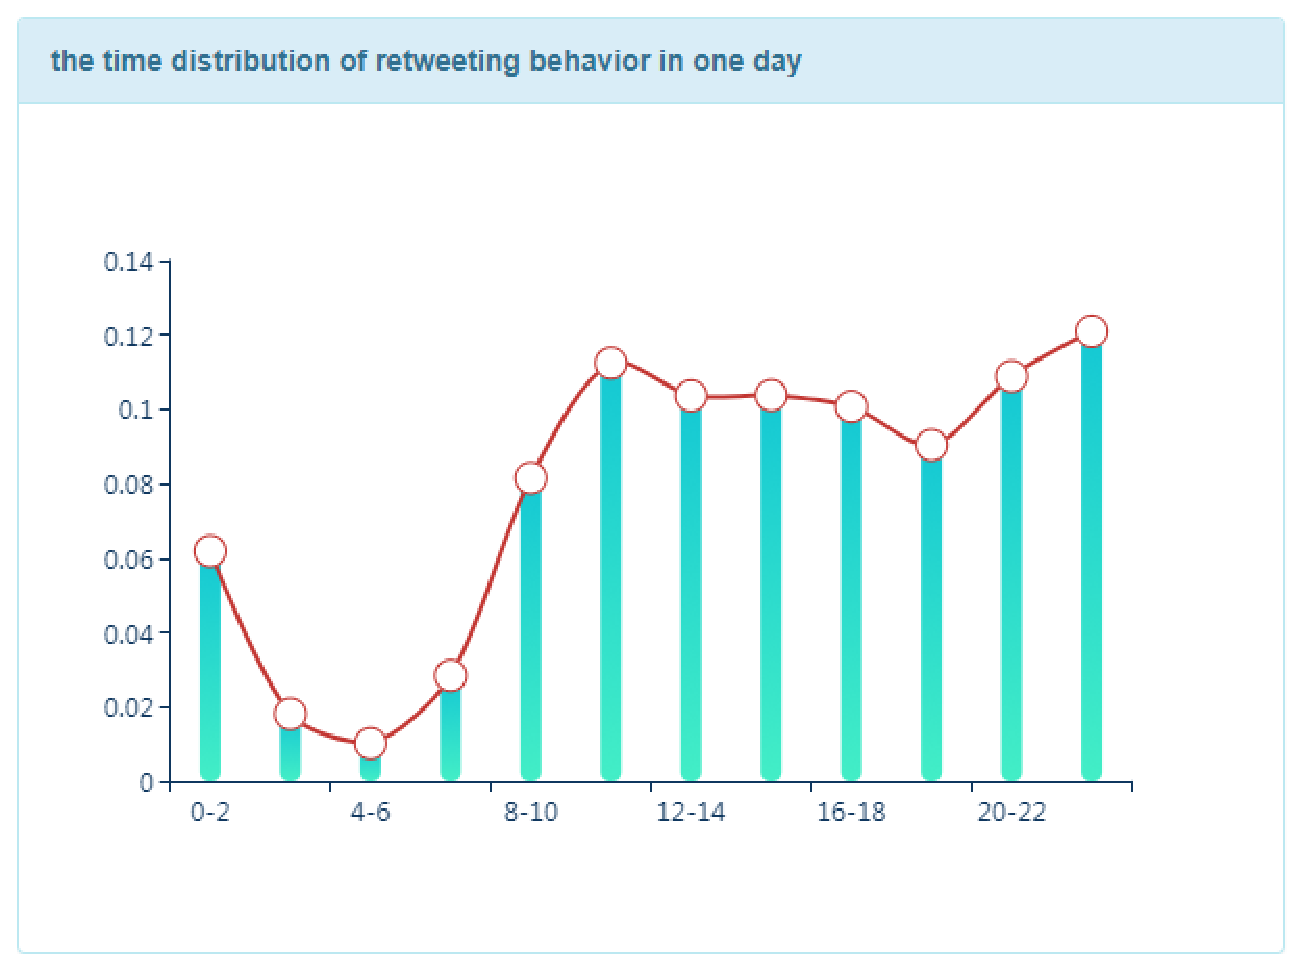
\includegraphics[width=0.23\textwidth]{IMAGE/group-images/26.eps}}
  \subfigure[]{
  \label{fig:subfig2:fig27}
      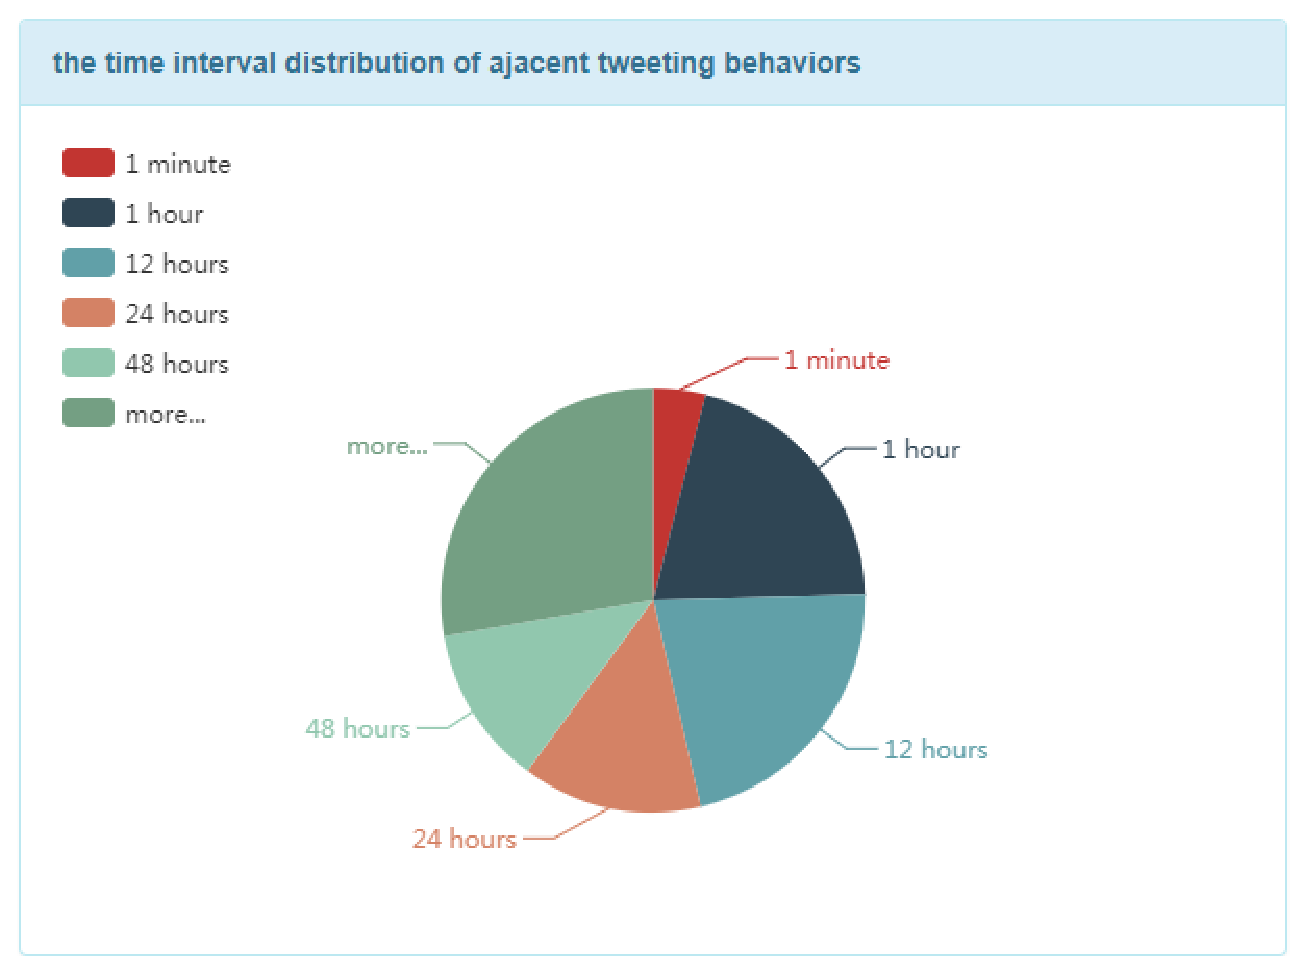
\includegraphics[width=0.23\textwidth]{IMAGE/group-images/27.eps}}
  \subfigure[]{
  \label{fig:subfig2:fig28}
      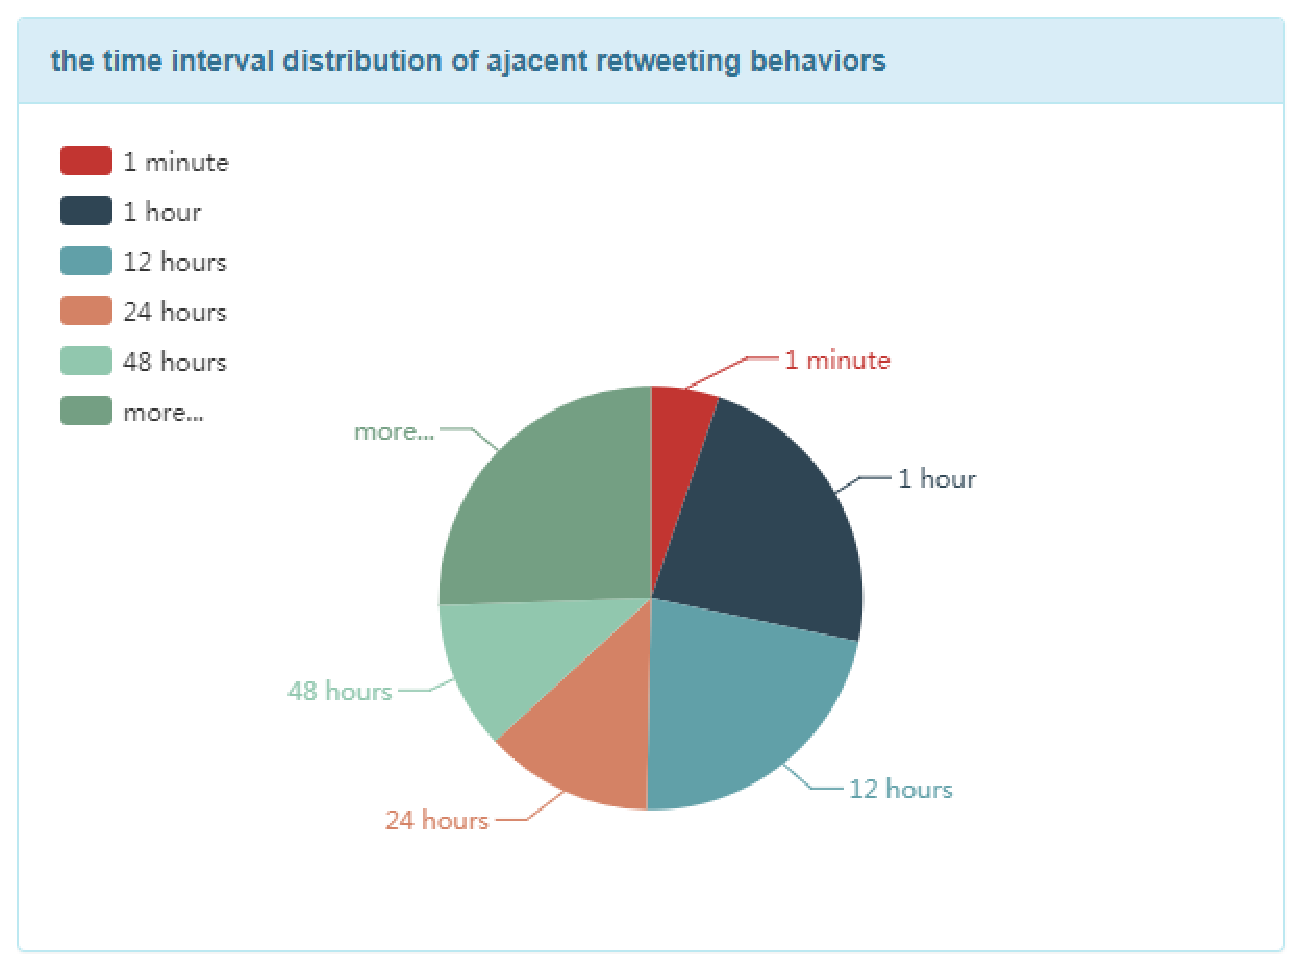
\includegraphics[width=0.23\textwidth]{IMAGE/group-images/28.eps}}
  \subfigure[]{
  \label{fig:subfig2:fig29}
      
\includegraphics[width=0.23\textwidth]{IMAGE/group-images/29.eps}}
  \caption{The Statistics of User Group Two}
  \label{fig:subfig2} %% label for entire figure
\end{figure*}

\begin{figure*}
  \centering
  \subfigure[]{
  \label{fig:subfig3:fig31}
      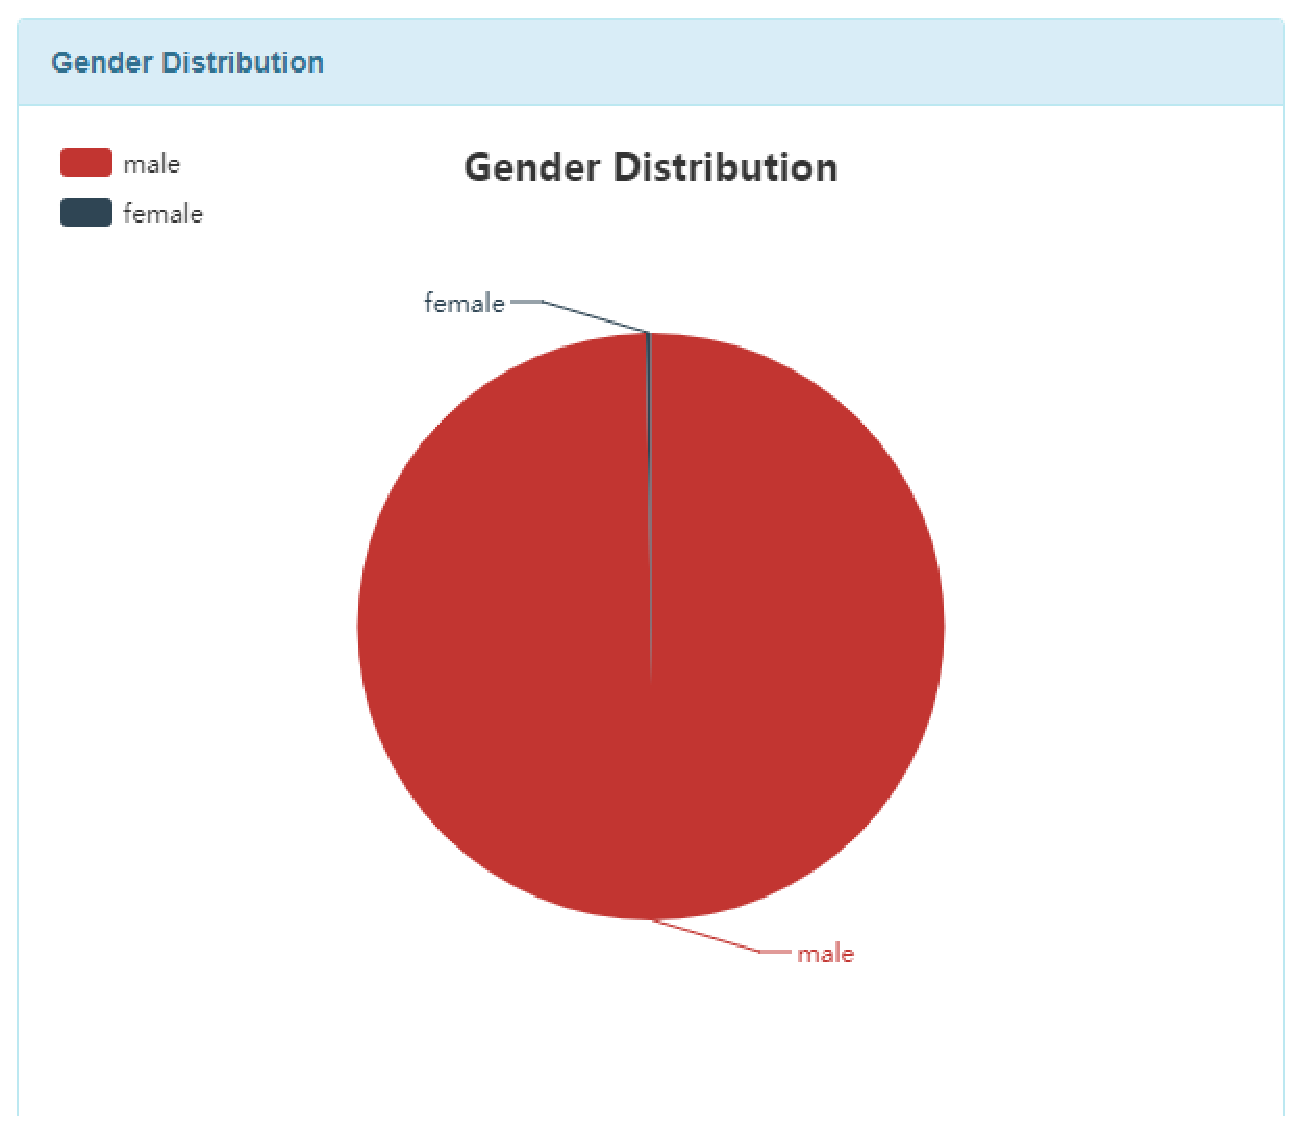
\includegraphics[width=0.23\textwidth]{IMAGE/group-images/31.eps}}
  \subfigure[]{
  \label{fig:subfig3:fig32}
      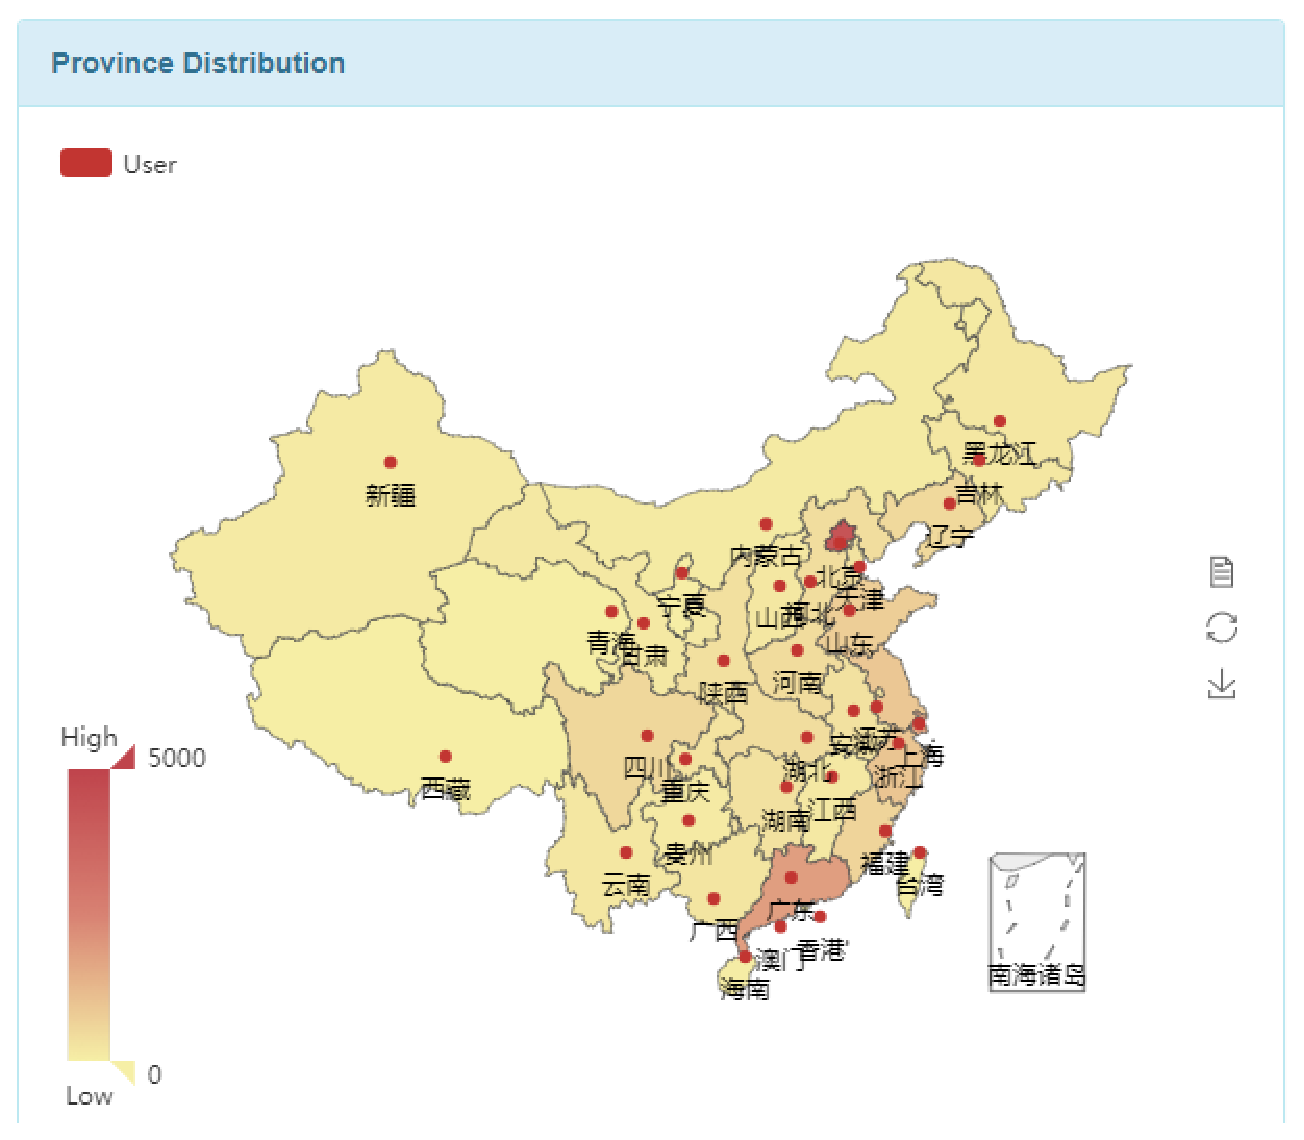
\includegraphics[width=0.23\textwidth]{IMAGE/group-images/32.eps}}
  \subfigure[]{
  \label{fig:subfig3:fig33}
      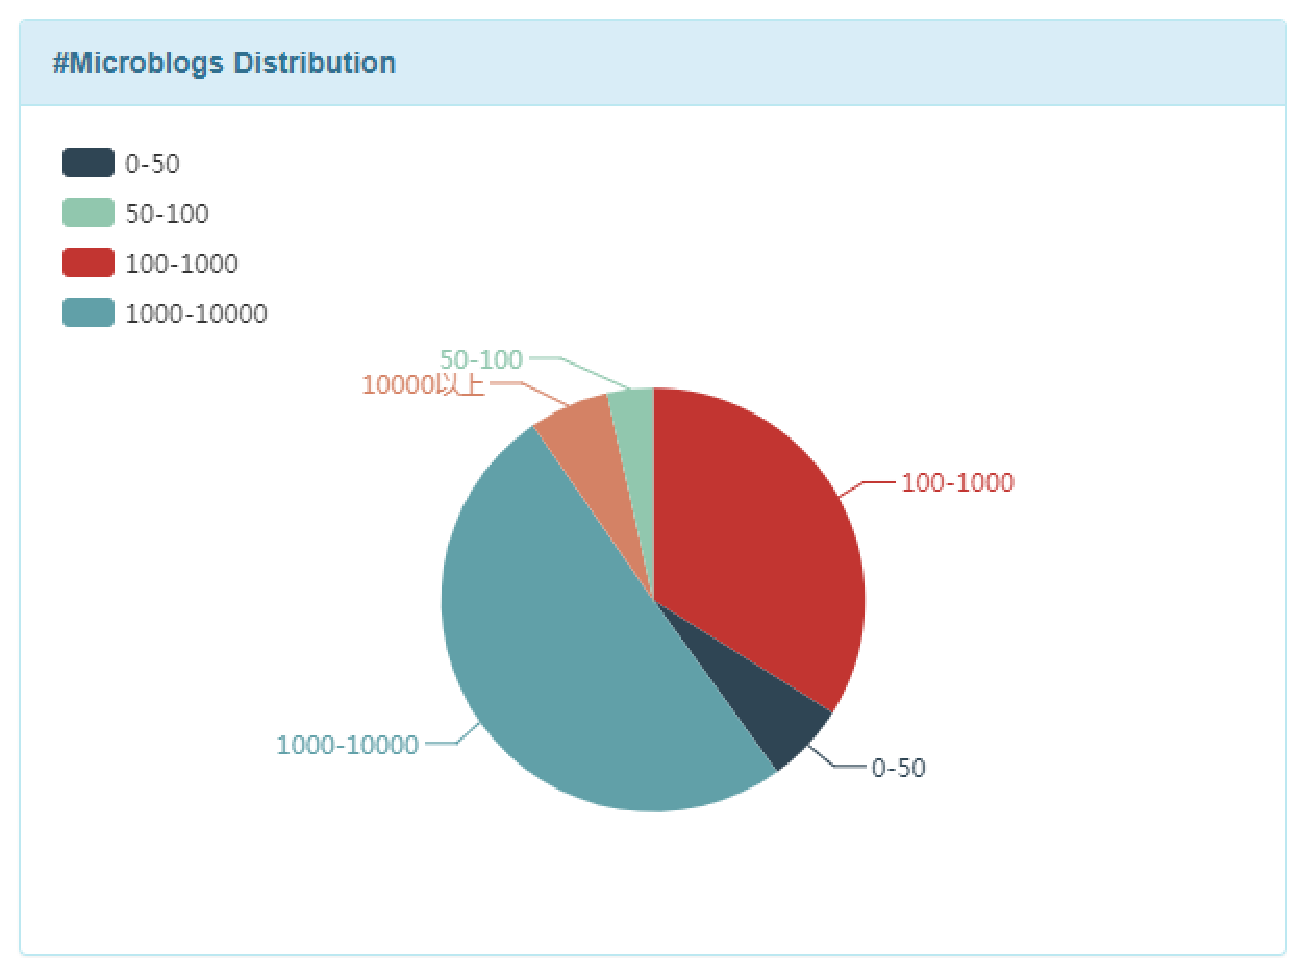
\includegraphics[width=0.23\textwidth]{IMAGE/group-images/33.eps}}
  \subfigure[]{
  \label{fig:subfig3:fig34}
      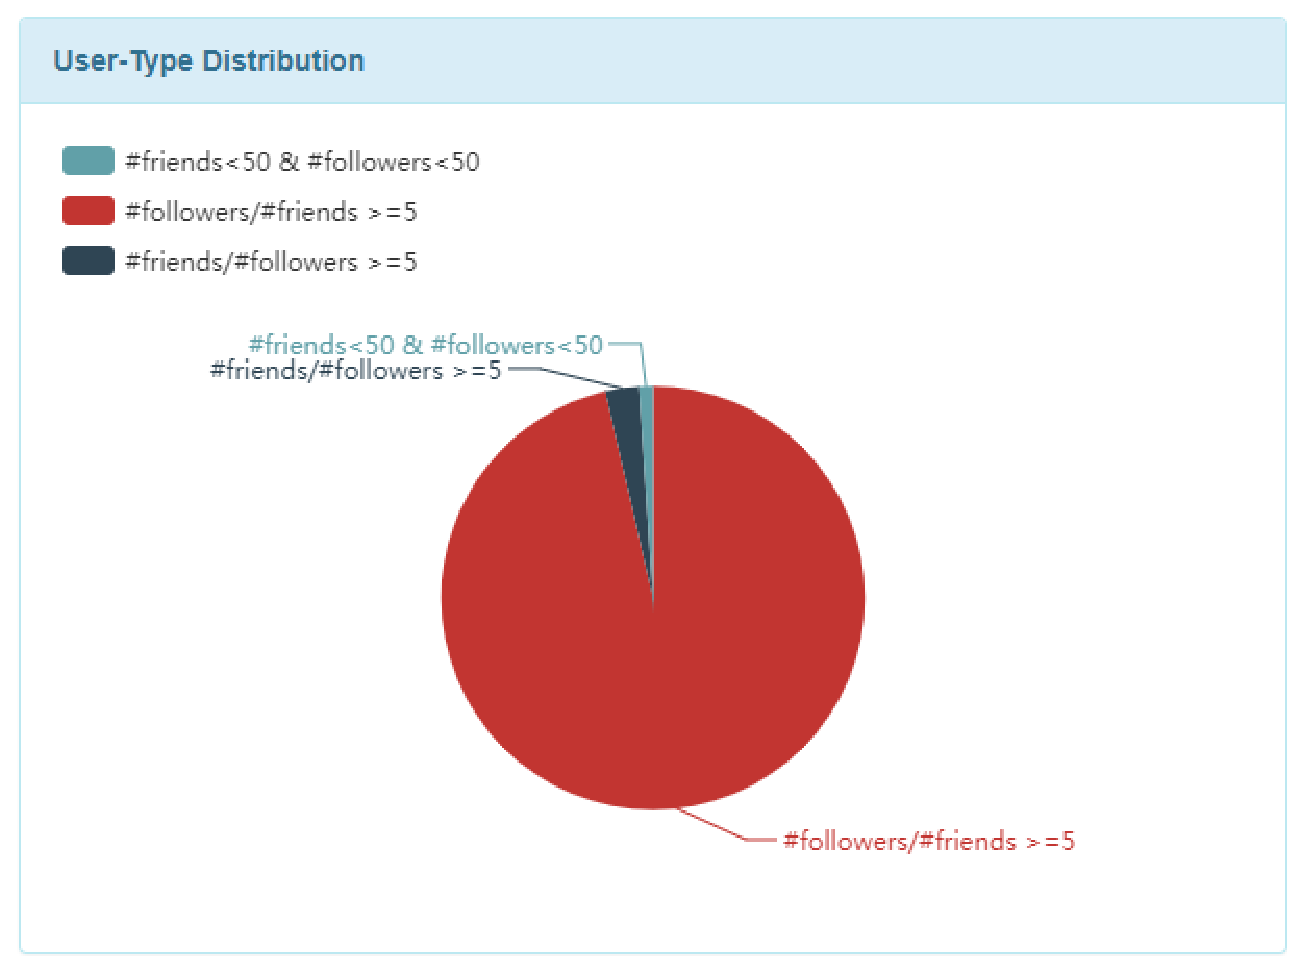
\includegraphics[width=0.23\textwidth]{IMAGE/group-images/34.eps}}
  \subfigure[]{
  \label{fig:subfig3:fig35}
      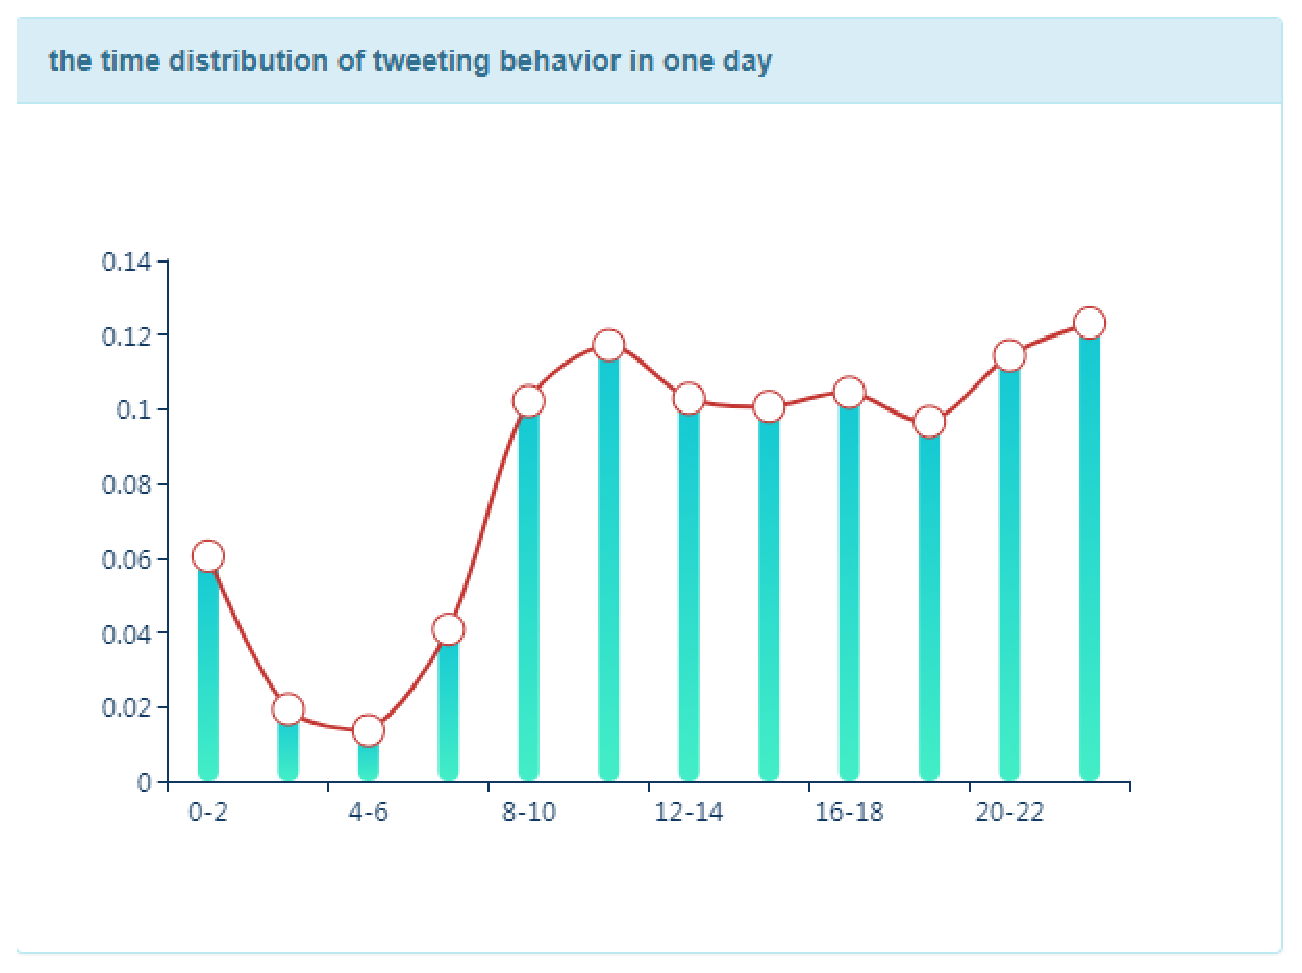
\includegraphics[width=0.23\textwidth]{IMAGE/group-images/35.eps}}
  \subfigure[]{
  \label{fig:subfig3:fig36}
      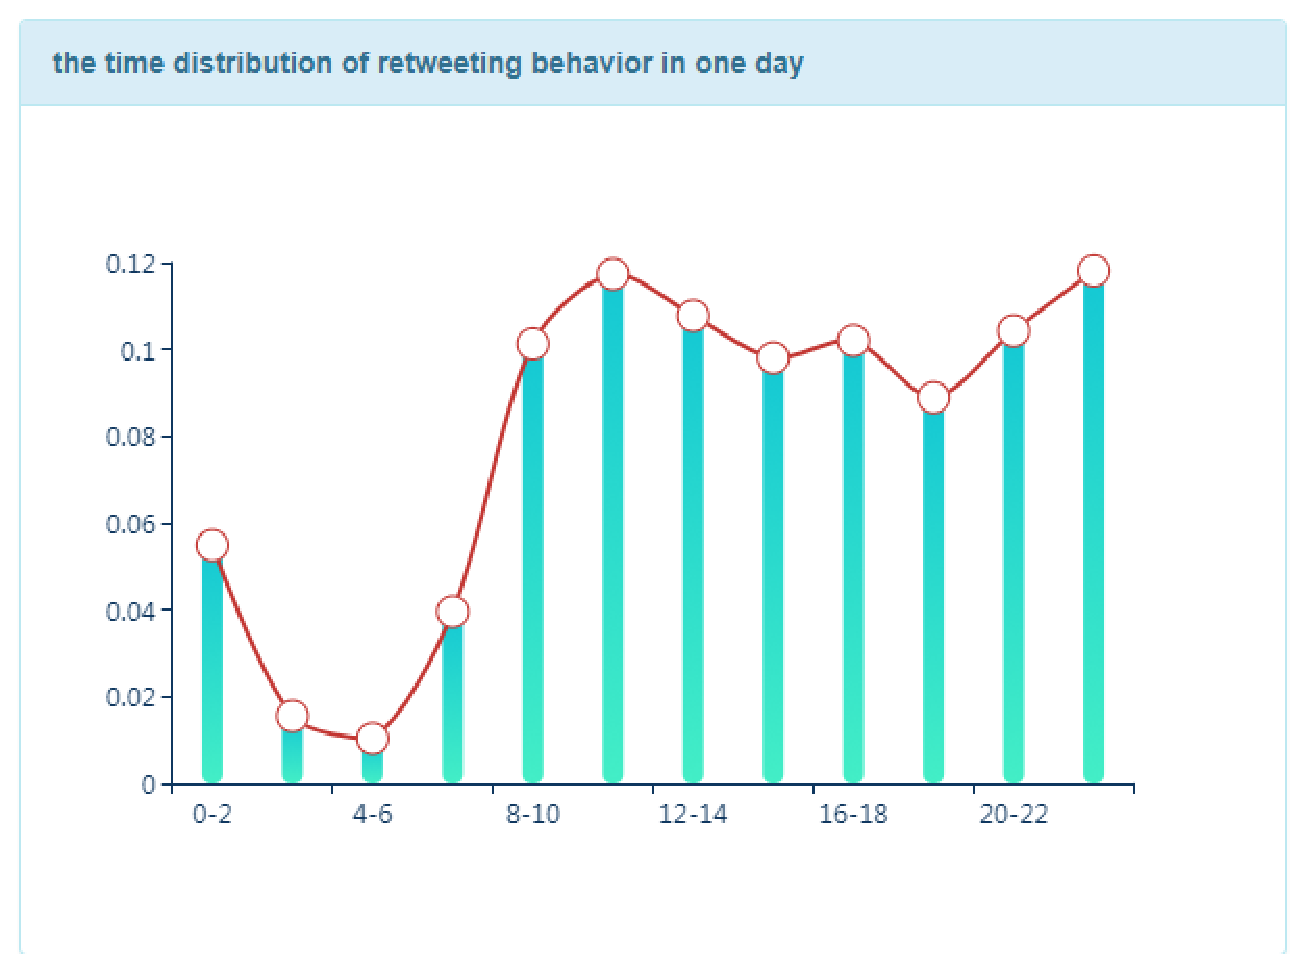
\includegraphics[width=0.23\textwidth]{IMAGE/group-images/36.eps}}
  \subfigure[]{
  \label{fig:subfig3:fig37}
      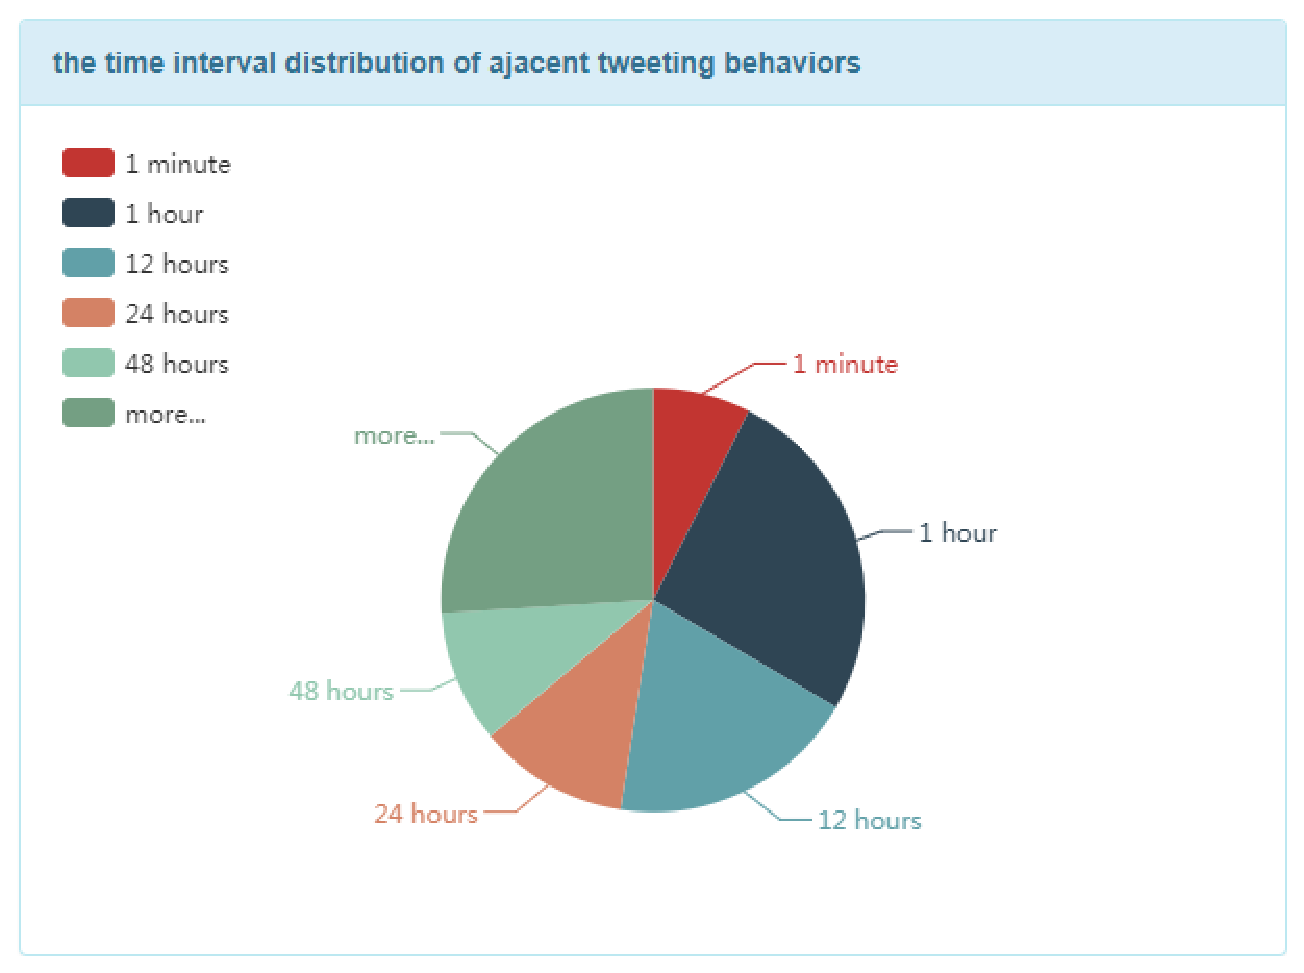
\includegraphics[width=0.23\textwidth]{IMAGE/group-images/37.eps}}
  \subfigure[]{
  \label{fig:subfig3:fig38}
      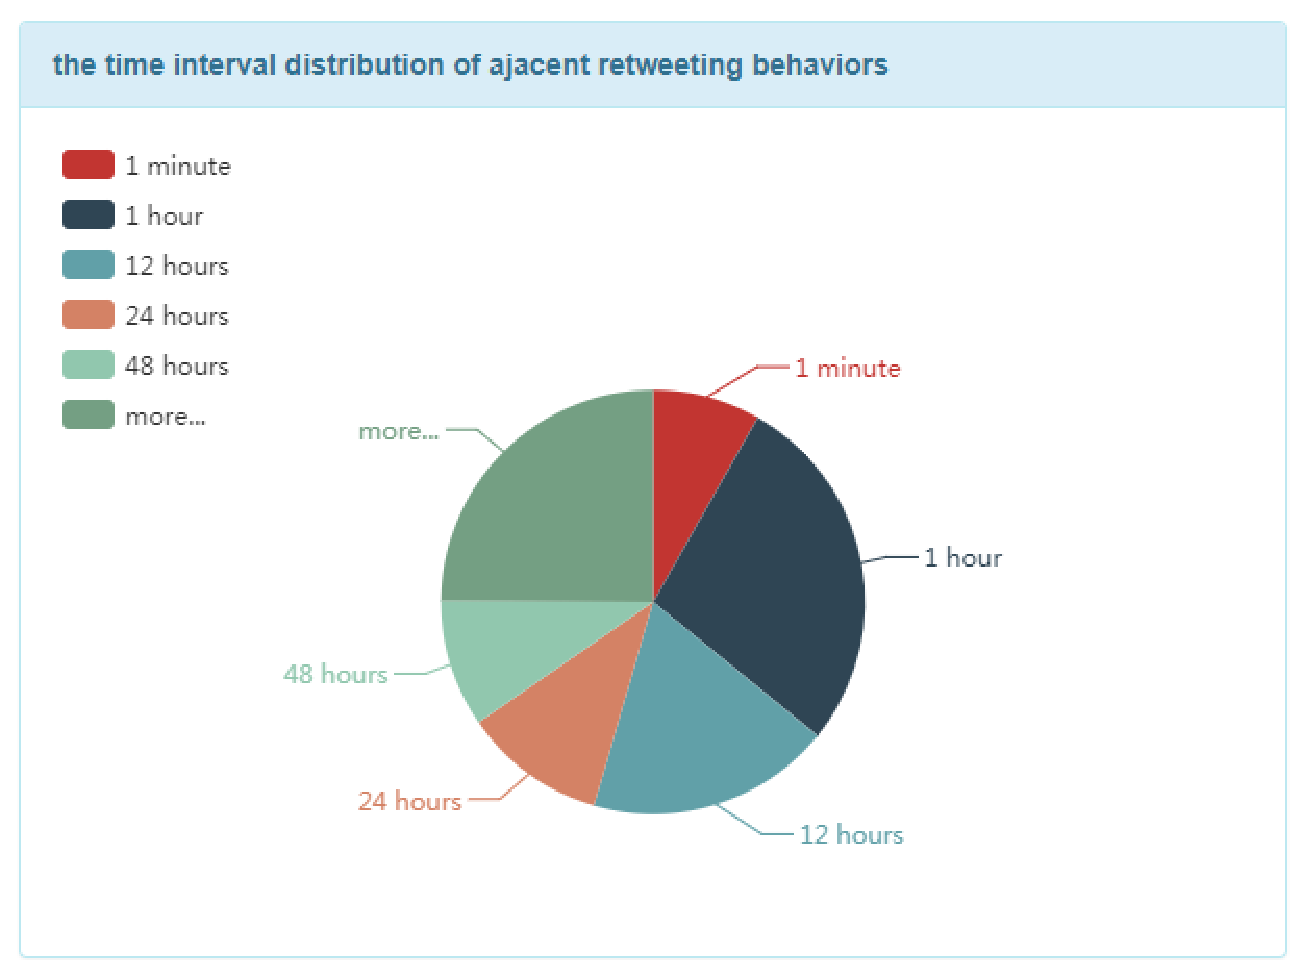
\includegraphics[width=0.23\textwidth]{IMAGE/group-images/38.eps}}
  \subfigure[]{
  \label{fig:subfig3:fig39}
      
\includegraphics[width=0.23\textwidth]{IMAGE/group-images/39.eps}}
  \caption{The Statistics of User Group Three}
  \label{fig:subfig3} %% label for entire figure
\end{figure*}


\begin{figure*}
  \centering
  \subfigure[]{
  \label{fig:subfig4:fig41}
      \includegraphics[width=0.23\textwidth]{IMAGE/group-images/41.eps}}
  \subfigure[]{
  \label{fig:subfig4:fig42}
      \includegraphics[width=0.23\textwidth]{IMAGE/group-images/42.eps}}
  \subfigure[]{
  \label{fig:subfig4:fig43}
      \includegraphics[width=0.23\textwidth]{IMAGE/group-images/43.eps}}
  \subfigure[]{
  \label{fig:subfig4:fig44}
      \includegraphics[width=0.23\textwidth]{IMAGE/group-images/44.eps}}
  \subfigure[]{
  \label{fig:subfig4:fig45}
      \includegraphics[width=0.23\textwidth]{IMAGE/group-images/45.eps}}
  \subfigure[]{
  \label{fig:subfig4:fig46}
      \includegraphics[width=0.23\textwidth]{IMAGE/group-images/46.eps}}
  \subfigure[]{
  \label{fig:subfig4:fig47}
      \includegraphics[width=0.23\textwidth]{IMAGE/group-images/47.eps}}
  \subfigure[]{
  \label{fig:subfig4:fig48}
      \includegraphics[width=0.23\textwidth]{IMAGE/group-images/48.eps}}
  \subfigure[]{
  \label{fig:subfig4:fig49}
      \includegraphics[width=0.23\textwidth]{IMAGE/group-images/49.eps}}
  \caption{The Statistics of User Group Four}
  \label{fig:subfig4} %% label for entire figure
\end{figure*}

\section{Related Work}
\label{sec:rela}

%In this section, we will introduce the related work of user modeling in social network from the aspects of user features analysis, user groups mining and user behaviors modeling. Social media users's features we mentioned here include users's basic information, behavior features and interests features.\par

%Users's basic information we mentioned here include the users's gender, age, region, occupation and other personal information. There are many researches for analyzing users's basic information, such as users's racial information analysis \cite{IEEEexample:conf/icwsm/PennacchiottiP11}, users's gender inference \cite{IEEEexample:conf/emnlp/CiotSR13}, users's actual age inference \cite{IEEEexample:conf/icde/ParkHHL09}, user policy orientation analysis (e.g. \cite{IEEEexample:conf/icwsm/PennacchiottiP11,IEEEexample:conf/acl/VolkovaCD14,IEEEexample:kosinski2013private}), user's geo-location and occupation mining \cite{IEEEexample:journals/tmm/FangSXH15,IEEEexample:conf/icde/FanCTWC16}, etc. Here, we did not do basic information mining for users. We used the user's basic information as important features for user clustering and behavior modeling. \par

%Social medias users's behaviors mainly refers to the tweeting and retweeting behaviors. Users's behaviors also have certain characteristics and regularity, which have been proved by a lot of existing work. Jiang et al. proposed a behavior dynamics model \cite{IEEEexample:jiang2013understanding}, theoretical analysis shows this model can properly explain various heavy-tailed inter-event time distributions, including a regular power law and some non-power-law deviations. Guo Z et al.\cite{IEEEexample:conf/music/GuoLTL12} analyzed the behavior of microblog users, the difference between the activity of users in different periods, and obtained the distribution of individual behavior on time. Pravallika Devineni et al. analyzed the wall activities of users focusing on identifying common patterns and proposed PowerWall distribution \cite{IEEEexample:journals/snam/DevineniKFF17}. What's more, it helped them spot surprising behaviors and anomalies. Considering the regularity of user behavior on time, we extracted characteristics of the user behavior as important features for user clustering and behavior modeling.\par

%As for users's interest, many methods has been proposed to do interests extraction. Zhiyuan et al.\cite{IEEEexample:journals/fcsc/LiuCS12} modeled users's interests through mining keywords. They extracted keywords from the users's microblogs by the combination of words frequency and translation model. Xu Z et al.\cite{IEEEexample:conf/webi/XuLXY11} proposed a method which extended user topic model to analyze users's interests. Michelson M et al.\cite{IEEEexample:conf/and/MichelsonM10} analyzed interests  based on a knowledge base. They used a knowledge base to identify and classify the entities in twitters of one user, then generate the user's interests category subtree to express his interests. Lim K H et al.\cite{IEEEexample:conf/wikis/LimD13} analyzed the celebrities a user mentioned, then they got the preference degree of the user in different interests categories. Bhattacharya P et al.\cite{IEEEexample:conf/recsys/BhattacharyaZGGG14} proposed a method to extract a user's interests by analyzing the experts he followed. By digging a list of certain topics of the custom experts the user follows, they got the user's interests profiling. Wei Feng et al.\cite{IEEEexample:conf/icde/FengW14} studied the methods mapping tweets to hashtags to get users's preferences for hashtags.  The existing methods for interest extraction have some shortcomings. The granularity of the result obtained by the methods based on keyword extraction is too small, and the result obtained by the user topic model is implicit and difficult to display. What's more, for the lack of a complete knowledge base, it's not easy to do interests extraction by using knowledge base. To solve the problems, we employed a cell lexicon to express user's interest. What's more, we combined Twitter-LDA \cite{IEEEexample:zhao2011comparing} and TF-IDF to extract the distribution of users's interest.\par

%There have also many studies on the user groups analysis. Some researches studied how to classify users under a specific situation. For instance, Marco Pennacchiotti et al.\cite{IEEEexample:conf/icwsm/PennacchiottiP11} classified users by race, political tendencies and so on.  \cite{IEEEexample:journals/tkdd/ZhangCFLYZY17} analyzed the evolution of social groups, such as Facebook groups and Wechat groups, and proposed a new model for group evolution, which can provide insights about different evolution patterns of social groups. Xin Wang et al. \cite{IEEEexample:conf/aaai/WangDNGEB16} implemented a time-varying factorization to measure the user-group affinity for recommending groups to users. In addition, research for users community mining is a hot spot. Jaewon Yang et al.\cite{IEEEexample:conf/wsdm/YangL13} proposed a method based on non-negative matrix decomposition to mine user community. Yiye Ruan et al.\cite{IEEEexample:conf/www/RuanFP13} considered user's friends and user's text content into their method when measuring the similarity between users for clustering. He et al. \cite{IEEEexample:he2014overlapping}
%only considered the relationship between friends, and used the edge aggregation coefficient as a measure of clustering. Hiroaki Shiokawa et al.\cite{IEEEexample:conf/aaai/ShiokawaFO13} used the modular degree as a clustering standard and proposed an incremental algorithm to mine user community. As we can see, current analysis of user groups are diverse. However, users in social networks have multiple features, and many existing methods do not take advantage of these features to group users. Here we took user's basic, behavioral and interest information into account when performing user clustering, and we got distinguish groups with different statistical characteristics.\par

%As for behavior modeling, Jing Zhang et al.\cite{IEEEexample:journals/tkdd/ZhangTLLX15} proposed a method of analyzing users's retweeting behavior from the perspective of influence. Some researchers (e.g. \cite{IEEEexample:conf/wsdm/FengW13}, \cite{IEEEexample:conf/ijcai/ZhangLTCL13}) find that the user's reposting behavior is largely influenced by the relationship between friends, so they consider user's friend structure information into their models. Bo Jiang et al. \cite{IEEEexample:conf/cikm/JiangLSW15} proposed a method that combined matrix decomposition and microblogs clustering to analyze the user's reposting behavior. Zhang et al.\cite{IEEEexample:zhang2015retweet} proposed non-parametric statistical models to combine structural, textual, and temporal information together to predict reposting behavior. Considering the situation that users's not reposting does not mean that users are not interested in it, the users may just did not see it, \cite{IEEEexample:conf/sigir/JiangLSLLMW16} applied a collaborative filtering method to the reposting behavior analysis. Maria Giatsoglou et al. explore the identification of fraudulent and genuine retweet threads and developed a realistic generator that mimics the behaviors of both honest and fraudulent users \cite{IEEEexample:conf/pakdd/GiatsoglouCSFV15}. Suhas Ranganath et al. \cite{IEEEexample:journals/corr/RanganathMHTL15} were inspired by sociological theories of protest participation and proposed a framework to predict from the user¡¯s past status messages and interactions whether the next post of the user will be a declaration of protest.  They evaluated the framework using data from Twitter on protests during the recent Nigerian elections and demonstrated that it could effectively work. Considering the fact that the amount of users in Social Medias is so huge, modeling for each user is not a good idea. However, modeling for a single user may make the model too particular. In addition, modeling for the whole users makes our model inaccuracy.
%So we divided users into several groups by users clustering. Then we get different behavior model for each group users respectively. \par


In this section, we shall review related work in literature mainly from the aspects of analyzing features, mining groups and modeling behavior within the realm of social network modeling.
As aforementioned, \sys{} leverages the user features of basic info, behavior and interest.

With respect to feature analysis, there have been existed works of mining users' info, such as race \cite{IEEEexample:conf/icwsm/PennacchiottiP11}, gender \cite{IEEEexample:conf/emnlp/CiotSR13}, age \cite{IEEEexample:conf/icde/ParkHHL09}, political preference \cite{IEEEexample:conf/icwsm/PennacchiottiP11,IEEEexample:conf/acl/VolkovaCD14,IEEEexample:kosinski2013private} and occupation \cite{IEEEexample:journals/tmm/FangSXH15,IEEEexample:conf/icde/FanCTWC16}.
Our work, however, does not focus on the mining process per se; we use the mined info as the input for user clustering and group modeling.

Studies of behavior analysis put emphasis on exploring the characteristics.
For example, \cite{IEEEexample:jiang2013understanding} proposed a model that can properly explain various time distributions of user behaviors by theoretical analysis;
\cite{IEEEexample:conf/music/GuoLTL12} studied the user activity distribution of one day/week;
\cite{IEEEexample:journals/snam/DevineniKFF17} provided the PowerWall distribution of Facebook users, identifying a number of surprising behaviors and anomalies.
Considering the behavior characteristics, \sys{} makes use of them to feed the modeling process.

There have been established work of extracting user interests.
\cite{IEEEexample:journals/fcsc/LiuCS12} mined the user interests by exploring keywords of microblogs with the aid of word frequency and machine translation.
\cite{IEEEexample:conf/webi/XuLXY11} proposed a method of extending the topic model to obtain use interests.
Also, \cite{IEEEexample:conf/and/MichelsonM10} used a knowledge base and \cite{IEEEexample:conf/icde/FengW14} provided a solution of using hashtag for interest analysis.
\cite{IEEEexample:conf/wikis/LimD13} summarized user interest by exploring the mentioned celebrities;
Similarly, \cite{IEEEexample:conf/recsys/BhattacharyaZGGG14} leveraged the followed experts to result interest characteristics.
Unlike the existed solutions, \sys{} employs a cell lexicon to properly express user interest in which Twitter-LDA \cite{IEEEexample:zhao2011comparing} and TF-IDF are employed.

Approaches of grouping users in social network could fall into a variety of categories.
\cite{IEEEexample:conf/icwsm/PennacchiottiP11} grouped users by the info of race, political view and etc.
\cite{IEEEexample:journals/tkdd/ZhangCFLYZY17} studied the social groups on Facebook and Wechat, resulting various patterns of group evolution.
\cite{IEEEexample:conf/aaai/WangDNGEB16} proposed a time-varying factor to measure the affinity between users and groups such that proper group proposals are recommended.
More recent studies also look into mining user communities.
\cite{IEEEexample:conf/wsdm/YangL13} employed matrix decomposition to mine user community;
\cite{IEEEexample:conf/www/RuanFP13} and \cite{IEEEexample:he2014overlapping} considered followees info for user clustering;
\cite{IEEEexample:conf/aaai/ShiokawaFO13} proposed an incremental algorithm to mine user community using modular degree as the clustering yardstick.
Providing the diversity of user features, \sys{} employs feature of info, behavior and interest into user clustering.

The main problem of current approaches for behavior modeling lies in that the model is for either the overall users or a single user.
\cite{IEEEexample:journals/tkdd/ZhangTLLX15, IEEEexample:conf/wsdm/FengW13, IEEEexample:conf/ijcai/ZhangLTCL13} discovered that users' \retg{} behavior is largely influenced by their followees, whereas \cite{IEEEexample:conf/cikm/JiangLSW15} employed matrix decomposition, \cite{IEEEexample:conf/sigir/JiangLSLLMW16} used collaborative filtering methods and \cite{IEEEexample:zhang2015retweet} leveraged statistical models for \retg{} analysis.
\cite{IEEEexample:conf/pakdd/GiatsoglouCSFV15} and \cite{IEEEexample:journals/corr/RanganathMHTL15} focused on identifying whether the \retg{} is fraudulent or of protest.
Whereas our work \sys{} builds the \retg{} model for each user group, instead of the mono model for all users or one model per user.


\section{Conclusions}
\label{sec:conclu}

In this work, we have presented \sys{}, a system to model the \retg{} behavior of users in social media.
\sys{} departures from existing work by grouping users into clusters, during which features of basics, behavior and interests are extracted.
Specially, we have studied interest features from various perspectives, such as long-term/short-term interests and explicit/implicit interests.
Finally, we have provided a performance evaluation of \sys{} by using real-world datasets to demonstrate the benefits of our system \sys{}.


\stitle{Acknowledgments}.
Ma is supported in part by NSFC U1636210, 973 Program 2014CB340300, NSFC 61421003, and  MSRA Collaborative Research Program.
Li is supported in part by NSFC U1636123 \& 61403090.
 For any correspondence, please refer to Shuai Ma.



\bibliographystyle{abbrv}
\balance
\begin{small}
\bibliography{zhu-dasfaa}
\end{small}



\end{CJK*}
\end{document}

% End of ltexpprt.tex
